\documentclass[11pt,a4paper,oneside]{report}
\usepackage[T1]{fontenc}
\usepackage[utf8]{inputenc}
\usepackage{lmodern}
\usepackage[margin=24mm,headheight=14pt]{geometry}
\usepackage{amsmath,amssymb,mathtools,mathrsfs}
\usepackage{booktabs,array,tabularx,longtable}
\usepackage{enumitem}
\usepackage{xcolor}
\usepackage{microtype}
\usepackage{tikz,pgfplots}
\usetikzlibrary{arrows.meta,positioning,calc}
\pgfplotsset{compat=1.18}
\usepackage[most]{tcolorbox}
\usepackage{graphicx}
\graphicspath{{Figures/}}
\usepackage{hyperref}
\definecolor{ink}{HTML}{17354B}
\definecolor{accent}{HTML}{267C84}
\definecolor{soft}{HTML}{EDF4F6}
\hypersetup{colorlinks=true,linkcolor=ink,urlcolor=accent,citecolor=ink,
pdftitle={Discrete-Time Quantum Walks in a Rectangular Billiard: Consolidated Teaching Notes},
pdfauthor={DQW project}}
\newcommand{\ket}[1]{\lvert #1\rangle}
\newcommand{\bra}[1]{\langle #1\rvert}
\newcommand{\HH}{\mathcal H}
\newcommand{\CC}{\mathcal C}
\newcommand{\Id}{I}
\newcommand{\Tr}{\operatorname{Tr}}
\newcommand{\diag}{\operatorname{diag}}
\newcommand{\spec}{\operatorname{spec}}
\newcommand{\spanof}{\operatorname{span}}
\newcommand{\norm}[1]{\left\lVert#1\right\rVert}
\newcolumntype{Y}{>{\raggedright\arraybackslash}X}
\newcommand{\sw}{\mathrm{SW}}
\newcommand{\rc}{\mathrm{RC}}
\newcommand{\exact}{\textbf{Exact result.}\ }
\newcommand{\recorded}{\textbf{Recorded numerical result.}\ }
\newcommand{\open}{\textbf{Unresolved.}\ }
\newcommand{\session}{\textbf{Computed for this revision.}\ }
\newtcolorbox{lesson}[1]{breakable,colback=soft,colframe=accent,
boxrule=.5pt,arc=1mm,left=3mm,right=3mm,top=2mm,bottom=2mm,
title={#1},fonttitle=\bfseries,coltitle=white}
\setlength{\parindent}{0pt}
\setlength{\parskip}{.45em}
\setlength{\emergencystretch}{2em}
\setlist{itemsep=2pt,topsep=4pt}
\renewcommand{\arraystretch}{1.15}
\setcounter{tocdepth}{1}
\renewcommand{\bibname}{References}
\numberwithin{equation}{chapter}

\begin{document}
\hypersetup{pageanchor=false}
\begin{titlepage}
\vspace*{18mm}
{\color{accent}\large DQW PROJECT\par}
\vspace{12mm}
{\color{ink}\Huge\bfseries Discrete-Time Quantum Walks\\[3mm]
in a Rectangular Billiard\par}
\vspace{10mm}
{\Large From the shift and the geometry\\
to the coin and the full Floquet operator\par}
\vspace{16mm}
{\large Notes on progress...\par}
\vspace{3mm}
\vfill
\begin{lesson}{The guiding question:}
Which structures are fixed by the shift and the rectangle, which of
them survive a chosen coin, and what can those surviving structures
tell us about exact solvability and spectral statistics?
\end{lesson}
\vspace{10mm}
29 October 2026
\end{titlepage}
\hypersetup{pageanchor=true}
\pagenumbering{roman}

\chapter*{A reading guide for the student}
\addcontentsline{toc}{chapter}{A reading guide for the student}

A coin, the shift, and a domain play different roles. These notes
construct the complete quantum walk in stages. The first four stages
identify what is present before a coin has been selected; the last three
read every coin through the same geometric lens and then ask how each
one breaks (or keeps) the exact solvability of the rectangle.
\begin{center}\small
\begin{tabularx}{\textwidth}{@{}lYY@{}}\toprule
Stage & Question & Ingredients fixed so far\\\midrule
1. Floquet structure & What do the two factors do?
& A finite position space and four internal states; no specified shift or coin\\
2. Shift & What happens on an allowed or blocked move?
& A moving, stay-and-reverse prescription on a general site set\\
3. Rectangle & Which cycles and reflections follow?
& The rectangle and the shift, with no coin chosen\\
4. The 16-cell map & What does the wall do to a pair of directions, and which coin amplitudes keep a standing wave intact?
& Coherent channels \(h_\pm,v_\pm\), their spatial envelopes, and the allowed/forbidden cells of a \(4\times4\) coin\\
5. Local coins & What does each explicit matrix do, read in the 16-cell map?
& Identity, permutation, Grover, Fourier, two Bell matrices, modified Grover, modified Bell\\
6. Full walks & Which structures survive, and what do the spectra and eigenstates show?
& Their ordered composition with the same rectangle and walls\\
7. Mechanisms & By which route does each coin leave exact solvability?
& The demonstrated reduction families and the coins placed among them\\\bottomrule
\end{tabularx}
\end{center}

\textbf{One main convention.} Directions are ordered \((R,L,U,D)\).
The same \(4\times4\) coin acts first at every site; the shift acts
second. On an existing link it keeps the direction label. On a blocked
move it stays at the site and reverses direction with amplitude \(+1\).
No periodic boundary or extra reflection phase is used. The older
flip-flop/self-loop model is kept separate (Appendix~\ref{app:legacy}).

\begingroup
\setlength{\parskip}{0pt}
\small
\tableofcontents
\endgroup

\clearpage
\pagenumbering{arabic}


\chapter{The Floquet operator before choosing its ingredients}
\label{ch:general}

\section{Position and the four internal states}

Let \(\Omega\) be a finite set of \(N\) allowed positions. At this
stage its shape has not been specified. A basis vector
\(\ket{\mathbf r,d}\) states both where the walker is and which
internal state it carries. The four internal labels will later be
associated with directions, in the fixed order
\[
(R,L,U,D).
\]
The state space is
\begin{equation}
\HH=\HH_{\mathrm{pos}}\otimes\HH_{\mathrm{coin}},\qquad
\HH_{\mathrm{coin}}=\mathbb C^4,\qquad
\dim\HH=4N\equiv D.
\end{equation}
The tensor product means that a basis state requires \emph{both}
a position label and an internal label. A general normalized state is
\begin{equation}
\ket{\psi_n}=\sum_{\mathbf r\in\Omega}\sum_d
\psi_d(\mathbf r,n)\ket{\mathbf r,d},\qquad
\sum_{\mathbf r,d}|\psi_d(\mathbf r,n)|^2=1.
\end{equation}
These coefficients are complex amplitudes. Different contributions to
the same final basis state add before their absolute square is taken.
This is why probabilities alone will not determine the walk.

\section{The onsite coin and the shift}

The coin is a unitary \(4\times4\) matrix \(C\). Throughout the main
model it is homogeneous: the same matrix acts at every site and every
step. Its full-space action is
\begin{equation}
\CC=\Id_{\mathrm{pos}}\otimes C,\qquad
\CC\ket{\mathbf r,a}=\sum_d C_{da}\ket{\mathbf r,d}.
\end{equation}
Rows of \(C\) label outputs and columns label inputs. The coin changes
the internal amplitudes at a fixed position.

The shift \(S\) is a second unitary operator on \(\HH\). Its matrix
has dimension \(D\times D\), not \(4\times4\). We have not yet
specified what move it implements or how it treats a boundary.
One complete step is
\begin{equation}
\boxed{U=S\CC=S(\Id_{\mathrm{pos}}\otimes C),\qquad
\ket{\psi_{n+1}}=U\ket{\psi_n}.}
\label{eq:step}
\end{equation}
Operators act from right to left: coin first, shift second. For any input,
\begin{equation}
U\ket{\mathbf r,a}=\sum_d C_{da}S\ket{\mathbf r,d}.
\label{eq:componentstep}
\end{equation}
The coin supplies local amplitudes and the shift transports their basis
states. This separates their jobs before a move is specified. A coin
is not a measurement and need not be random.
In general \(S\CC\neq\CC S\), so the order must be stated.

\section{Why the repeated step is called Floquet evolution}

The same update is repeated at each integer time, so after \(n\)
steps \(\ket{\psi_n}=U^n\ket{\psi_0}\). We call \(U\) the
Floquet, or one-period, operator. Its eigenvalues are phases:
\begin{equation}
U\ket{\phi_j}=e^{i\varphi_j}\ket{\phi_j},\qquad
\varphi_j\equiv\varphi_j+2\pi.
\end{equation}
If a period \(T\) and \(\hbar=1\) are introduced, the convention
\(U=e^{-iH_{\mathrm{eff}}T}\) identifies
\(\varepsilon_j=-\varphi_j/T\), modulo \(2\pi/T\). The walk is
specified directly by its step; no particular continuous Hamiltonian
or continuous-time approximation is assumed.

\section{What follows from unitarity alone}

Because both factors are unitary,
\begin{equation}
U^\dagger U
=\CC^\dagger S^\dagger S\CC=\Id.
\end{equation}
Thus probability is conserved, evolution is reversible, and \(U\)
has an orthonormal eigenbasis. Its eigenphases lie on a circle.
These are the general conclusions available before specifying either
factor. Unitarity alone gives neither spatial separability nor a
particular reflection symmetry, time-reversal symmetry, or spectral
statistics.

\section{Conserved subspaces and direct sums}
A conserved observable \(Q\) satisfies
\begin{equation}
[U,Q]=UQ-QU=0.
\end{equation}
Then its expectation value is constant. A conserved subspace can be
described by an orthogonal projector \(P\):
\begin{equation}
P^2=P=P^\dagger,\qquad [U,P]=0.
\end{equation}
For a unitary \(U\), this means that both the subspace and its
orthogonal complement are invariant.

One sufficient way to conserve \(Q\) is to have
\([S,Q]=[\CC,Q]=0\). This is not a necessary condition for an
arbitrary \(Q\): the two factors can also combine to preserve a
structure neither preserves separately. We must examine the full step.

For mutually orthogonal conserved projectors summing to identity,
\[
\HH=\bigoplus_a\HH_a,\qquad
\HH_a=\operatorname{im}P_a,\qquad U=\bigoplus_a U_a.
\]
The image is the subspace selected by the projector. This groups
alternative state components, not different particles. A tensor product
still specifies the labels of a state.

Every finite unitary has its eigenprojectors. Their existence alone
cannot distinguish exact solvability from complicated dynamics. The
project's useful reductions are constructed from transport, geometry
and the coin before diagonalizing the full walk. A few parity blocks
whose dimensions grow with the area are not a complete solution.

\section{Keeping the operator sizes distinct}

\begin{center}\small
\begin{tabularx}{\textwidth}{@{}lYY@{}}\toprule
Object & Space on which it acts & Matrix size\\\midrule
Local coin \(C\) & Four internal states & \(4\times4\)\\
Local direction observable \(q\) or reversal \(J\) & Four internal states & \(4\times4\)\\
Full coin \(\CC=\Id_{\mathrm{pos}}\otimes C\) & Position and direction & \(D\times D\)\\
Shift \(S\), full step \(U\), full symmetry or projector & Position and direction & \(D\times D\)\\
Restricted operator \(U_a\) & A sector of rank \(r_a\) & \(r_a\times r_a\)\\\bottomrule
\end{tabularx}
\end{center}
The rank of a projector is the dimension of its image, not the number
of rows of the projector matrix. A local direction operation is extended
by the position identity before it is compared with the shift. These
distinctions will be important when a four-dimensional coin block is
compared with a full-space standing-wave block.

\begin{lesson}{What we have learned}
A walk state carries position and coin information. The coin acts
onsite, the shift implements transport, and their ordered product is
the Floquet step. Exact solvability or quantum-chaotic spectral
behavior is a property of that product with its boundary convention.
\end{lesson}


\chapter{The shift: transport, boundaries, and reversal}
\label{ch:shift}

\section{One move and one boundary rule}

We now choose the transport prescription while keeping the allowed-site
set arbitrary. The notation \(S_\Omega\) makes its domain dependence
explicit: different site sets can give different cycles and symmetries.

Associate the internal labels with displacements
\[
\delta_R=(1,0),\quad \delta_L=(-1,0),\quad
\delta_U=(0,1),\quad \delta_D=(0,-1).
\]
Let \(\bar d\) be the opposite direction:
\(\bar R=L\), \(\bar L=R\), \(\bar U=D\), \(\bar D=U\).
The main shift is
\begin{equation}
\boxed{
S_\Omega\ket{\mathbf r,d}=
\begin{cases}
\ket{\mathbf r+\delta_d,d},&\mathbf r+\delta_d\in\Omega,\\
\ket{\mathbf r,\bar d},&\mathbf r+\delta_d\notin\Omega.
\end{cases}}
\label{eq:moving}
\end{equation}
At an allowed move, the walker travels one site and keeps its
direction. At a blocked move it stays where it is and reverses its
direction. A boundary event therefore consumes one step of the shift.
Every displayed amplitude is \(+1\); no reflection phase or loss is
included. The rule is applied linearly to each component of a superposition.
Arriving at the last allowed site does not reverse the label. The
reversal occurs on the attempted outward shift. There is no state at
a nonexistent site.

The discrete geometry is the allowed-site set together with its
nearest-neighbor links. A wall is represented by a missing link.
There is no periodic identification. The rule does not require a
continuous normal vector; in particular, a corner presents two
different blocked directional channels.

\section{Why this shift is unitary}

The shift sends each position--direction basis state to precisely one
basis state with amplitude one. It is also one-to-one. To find the
predecessor of \(\ket{\mathbf r,d}\), ask whether
\(\mathbf r-\delta_d\) is allowed. If it is, the predecessor is
\(\ket{\mathbf r-\delta_d,d}\). If it is not, the predecessor is
\(\ket{\mathbf r,\bar d}\), whose attempted move is blocked.

Thus \(S_\Omega\) permutes the basis. Its matrix is real, with one
entry one in each row and column:
\begin{equation}
\boxed{S_\Omega^{-1}=S_\Omega^{\mathsf T}=S_\Omega^\dagger.}
\end{equation}
A finite permutation decomposes into disjoint cycles. Following a cycle
here means repeatedly applying \(S_\Omega\) \emph{alone}. The coin
will be inserted between successive shifts in the actual walk, and
may transfer amplitude between these cycles.

\section{What is fixed before choosing the shape?}

The prescription already gives a real unitary permutation and finite
basis cycles. It preserves the horizontal/vertical axis because
opposite-direction reversal does not change the axis. Cycle lengths
and spatial reflections depend on the site set. One further identity
is independent of its shape.

\section{Direction reversal reverses the shift}

Define the local reversal matrix
\begin{equation}
J=
\begin{pmatrix}
0&1&0&0\\1&0&0&0\\0&0&0&1\\0&0&1&0
\end{pmatrix},\qquad J^2=\Id_4.
\end{equation}
Write \(\mathcal J=\Id_{\mathrm{pos}}\otimes J\). The established
identity for the reflecting shift is
\begin{equation}
\boxed{\mathcal J S_\Omega\mathcal J=S_\Omega^{-1}.}
\label{eq:reverser}
\end{equation}
Reverse the direction, apply the move, and reverse again: this retraces
the original move, including a blocked move. Importantly,
Eq.~\eqref{eq:reverser} is a \emph{reversing relation}, not a statement
that \(\mathcal J\) commutes with the shift.

Since the shift is real, complex conjugation \(K\) obeys \(KSK=S\).
Combining it with reversal gives
\((\mathcal J K)S(\mathcal J K)^{-1}=S^{-1}\), with
\((\mathcal J K)^2=\Id\). This is a time-reversal relation for the
shift alone. Chapter~\ref{ch:assembled} explains why the corresponding
test for the full walk must also include the coin.

The earlier sessions also used a different, involutive flip-flop shift.
Its full comparison with this transport rule is retained in
Appendix~\ref{app:legacy}. We keep the present prescription fixed
throughout the main teaching sequence.

\chapter{The reflecting rectangle before a coin is chosen}
\label{ch:rectangle}

\section{Sites, dimensions, and the four edge rules}

We choose the site set, not yet the coin. Unless a square control
is identified, \(N_x\ne N_y\). The indices count sites, rather than
separately specified continuum side lengths. Fix
\begin{equation}
\Omega=\{1,\ldots,N_x\}\times\{1,\ldots,N_y\},\qquad
N=N_xN_y,\qquad D=4N_xN_y.
\end{equation}
For example, the horizontal rules become
\begin{align}
S\ket{x,y,R}&=
\begin{cases}\ket{x+1,y,R},&x<N_x,\\\ket{N_x,y,L},&x=N_x,\end{cases}\\
S\ket{x,y,L}&=
\begin{cases}\ket{x-1,y,L},&x>1,\\\ket{1,y,R},&x=1.\end{cases}
\end{align}
The vertical rules are
\begin{align}
S\ket{x,y,U}&=\begin{cases}\ket{x,y+1,U},&y<N_y,\\\ket{x,N_y,D},&y=N_y,\end{cases}\\
S\ket{x,y,D}&=\begin{cases}\ket{x,y-1,D},&y>1,\\\ket{x,1,U},&y=1.\end{cases}
\end{align}
At a corner its two outward components reverse independently.
There is no diagonal move. Horizontal motion preserves \(y\);
vertical motion preserves \(x\), yielding the first invariant
decomposition.

\section{Rows and columns are independent cycles of the shift}

For a fixed row and a fixed column define
\begin{align}
\HH_y^{H}
&=\spanof\{\ket{x,y,R},\ket{x,y,L}:1\leq x\leq N_x\},\\
\HH_x^{V}
&=\spanof\{\ket{x,y,U},\ket{x,y,D}:1\leq y\leq N_y\}.
\end{align}
Their dimensions are \(2N_x\) and \(2N_y\), respectively. They are
mutually orthogonal because their position--direction basis states
are distinct. They exhaust the full basis, so
\begin{equation}
\boxed{
\HH=\left(\bigoplus_{y=1}^{N_y}\HH_y^H\right)
\oplus\left(\bigoplus_{x=1}^{N_x}\HH_x^V\right).
}
\label{eq:rowsum}
\end{equation}
Each of these spaces is invariant under \(S\).

The row projectors are explicit full-space matrices:
\begin{equation}
P_y^H=\sum_{x=1}^{N_x}\sum_{d\in\{R,L\}}
\ket{x,y,d}\bra{x,y,d},
\end{equation}
and \(P_x^V\) is defined analogously. They satisfy
\([S,P_y^H]=[S,P_x^V]=0\) and sum to \(\Id_D\).
The coarser axis projectors are
\[
P_H=\sum_yP_y^H=\Id_{\mathrm{pos}}\otimes\diag(1,1,0,0),
\qquad P_V=\Id-P_H.
\]

On one row the basis states occur in the cycle
\begin{equation}
\ket{1,y,R}\to\cdots\to\ket{N_x,y,R}
\to\ket{N_x,y,L}\to\cdots\to\ket{1,y,L}\to\ket{1,y,R}.
\end{equation}
Its length is \(2N_x\). Each column similarly has length \(2N_y\).

\begin{figure}[htbp]
\centering
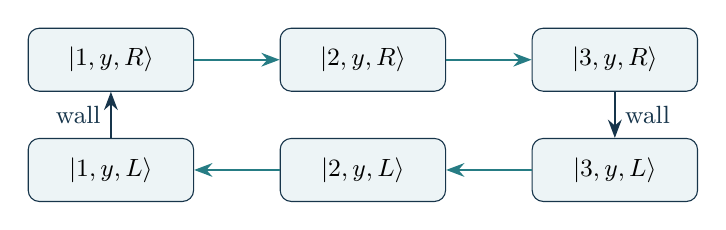
\begin{tikzpicture}[>=Stealth, every node/.style={font=\small},
state/.style={draw=ink,rounded corners,minimum width=21mm,
minimum height=8mm,fill=soft}]
\node[state] (a) at (0,1.4) {\(\ket{1,y,R}\)};
\node[state] (b) at (3.2,1.4) {\(\ket{2,y,R}\)};
\node[state] (c) at (6.4,1.4) {\(\ket{3,y,R}\)};
\node[state] (d) at (6.4,0) {\(\ket{3,y,L}\)};
\node[state] (e) at (3.2,0) {\(\ket{2,y,L}\)};
\node[state] (f) at (0,0) {\(\ket{1,y,L}\)};
\draw[->,thick,accent] (a)--(b);
\draw[->,thick,accent] (b)--(c);
\draw[->,thick,accent] (d)--(e);
\draw[->,thick,accent] (e)--(f);
\draw[->,thick,ink] (c)--node[right]{wall}(d);
\draw[->,thick,ink] (f)--node[left]{wall}(a);
\end{tikzpicture}
\caption{One shift cycle for a row of three sites. A wall arrow reverses
the direction at the same site. The diagram describes repeated shifts;
it does not yet include the action of an intervening coin.}
\end{figure}

If a cycle has basis \(\ket{j}\), \(j=0,\ldots,L-1\), with
\(S\ket{j}=\ket{j+1\bmod L}\), its Fourier vectors are
\begin{equation}
\ket{k}=\frac1{\sqrt L}\sum_{j=0}^{L-1}e^{-2\pi i kj/L}\ket{j},
\qquad S\ket{k}=e^{2\pi i k/L}\ket{k}.
\end{equation}
Thus the rectangular shift is exactly diagonalizable. Its order is
\begin{equation}
\boxed{S^{\,2\operatorname{lcm}(N_x,N_y)}=\Id.}
\end{equation}
The displayed exponent is its minimal positive period. It is not a
periodicity statement for a general \(U=S\CC\).

\section{Why a direct sum does not replace the tensor product}

The same space can be written as
\[
\HH=\HH_x\otimes\HH_y\otimes\mathbb C^4.
\]
This describes which labels specify a state. Equation~\eqref{eq:rowsum}
instead groups alternative sets of basis states on which the shift acts
independently. These are compatible descriptions.

For a decomposition \(\ket\psi=\sum_a\ket{\psi_a}\),
\(\ket{\psi_a}\in\HH_a\), a block-diagonal operator evolves each
component within its own \(\HH_a\). It does not describe several
independent walkers. The dimension check is
\[
N_y(2N_x)+N_x(2N_y)=4N_xN_y.
\]
Multiplying row-space and column-space dimensions would describe a
different system.

\section{Reflections must act on positions and directions}
\label{sec:rectsym}

A geometric reflection must also reflect the direction vector. Define
\begin{align}
\mathcal P_x\ket{x,y,d}
&=\ket{N_x+1-x,y,\sigma_x(d)},\\
\mathcal P_y\ket{x,y,d}
&=\ket{x,N_y+1-y,\sigma_y(d)},
\end{align}
where \(\sigma_x\) exchanges only \(R,L\), and \(\sigma_y\)
exchanges only \(U,D\). Let
\begin{equation}
\mathcal R=\mathcal P_x\mathcal P_y,\qquad
\mathcal R\ket{x,y,d}
=\ket{N_x+1-x,N_y+1-y,\bar d}.
\end{equation}
The rectangle and the moving shift obey
\begin{equation}
\boxed{[S,\mathcal P_x]=[S,\mathcal P_y]=[S,\mathcal R]=0.}
\end{equation}
These are real commuting involutions. For a nonsquare rectangle their
geometric group is
\(D_2=\{\Id,\mathcal P_x,\mathcal P_y,\mathcal R\}\), of order four.
This is the geometric group of the rectangle, not the entire operator
commutant of \(S\). Repeated cycles and degeneracies allow additional
shift-only conserved operators. The common-commutant formulation in
Appendix~\ref{app:advanced} covers that broader question.
The simultaneous parity projectors are
\begin{equation}
\Pi_{p_xp_y}=\frac14(\Id+p_x\mathcal P_x)(\Id+p_y\mathcal P_y),
\qquad p_x,p_y\in\{+1,-1\}.
\end{equation}
The commutators hold at the wall as well as in the bulk. A reflected
existing link remains existing, with its direction reflected. A
reflected blocked link stays blocked, and reflection and opposite-direction
reversal are compatible. Thus both orders of action agree on every
basis state. Position reflection alone or direction permutation alone
generally would not have this property.

Their ranks can be large. A one-dimensional group representation means
that each symmetry acts by a number \(\pm1\); it does \emph{not}
mean the entire symmetry sector has dimension one.

Since \(\mathcal R\) has no fixed position--direction basis states,
\(\Tr\mathcal R=0\). Its two projectors
\(\Pi_\pm=(\Id\pm\mathcal R)/2\) have equal rank \(2N\).
For a square, diagonal reflection is available as well and the full
geometric group is \(D_4\). One must then check which of those
operations also survive the coin.

The same geometry provides reversing operators:
\begin{equation}
P\in\{\mathcal J,\mathcal P_x\mathcal J,
\mathcal P_y\mathcal J,\mathcal R\mathcal J\}
\quad\Longrightarrow\quad PSP=S^{-1}.
\label{eq:allreversers}
\end{equation}
The last operator reflects both position coordinates and leaves the
direction label unchanged. These operators will enter the full-walk
time-reversal test in Chapter~\ref{ch:assembled}.

\section{Homogeneous bulk motion does not restore translation symmetry}

The coin will be homogeneous, but the finite rectangle has walls.
Translating a state by one site does not generally preserve the allowed
set and its edge rule. The finite walk therefore has no automatic
periodic translation symmetry or globally conserved plane-wave momentum.

Away from the walls, a plane wave can still be used to describe local
bulk evolution. Its matrix is
\begin{equation}
U(k_x,k_y)=\Lambda(k_x,k_y)C,\qquad
\Lambda=\diag(e^{-ik_x},e^{ik_x},e^{-ik_y},e^{ik_y}).
\end{equation}
The wall equations must then be imposed separately. The existence of
this bulk matrix is not a finite-rectangle separability theorem.


\chapter{Coherent channels, envelopes, and the 16-cell map of a coin}
\label{ch:sixteen}

\section{The question of this chapter}

The shift on the rectangle, with no coin yet, supports standing waves:
complete sets of states that the shift keeps inside small, explicitly
known subspaces (constructed in Sections~\ref{sec:standing} and
\ref{sec:projectors} below). Grover's exact
solution (Section~\ref{sec:groverfull}) works because Grover's coin also
keeps those subspaces. This chapter turns that observation into a test
that can be applied to \emph{any} coin, \emph{before} the full walk is
diagonalized:
\begin{lesson}{Question}
Given only the \(4\times4\) coin matrix \(C\), does the full walk
\(U=S(\Id_{\mathrm{pos}}\otimes C)\) keep the standing waves of the
rectangle, and if not, how much of each wave does it lose per step?
\end{lesson}
The answer requires three ingredients, developed in order:
\begin{enumerate}
\item a basis of the four internal states adapted to the walls, the
\emph{coherent channels} (Section~\ref{sec:panela});
\item the notion of the \emph{envelope} of a state, and the rule that
assigns an envelope to each coherent channel
(Sections~\ref{sec:envelopedef}--\ref{sec:projectors});
\item the observation that a coin can change the internal state but never
the envelope. As a result, everything is decided by the sixteen entries of
\(C\) written in the coherent basis (Sections~\ref{sec:whysquare}--\ref{sec:envelope}).
\end{enumerate}
Figure~\ref{fig:wallmask} summarizes the three steps. Its panels (a), (b)
and (c) correspond to Sections~\ref{sec:panela}, \ref{sec:panelb} and
\ref{sec:envelope}.

\begin{figure}[htbp]
\centering
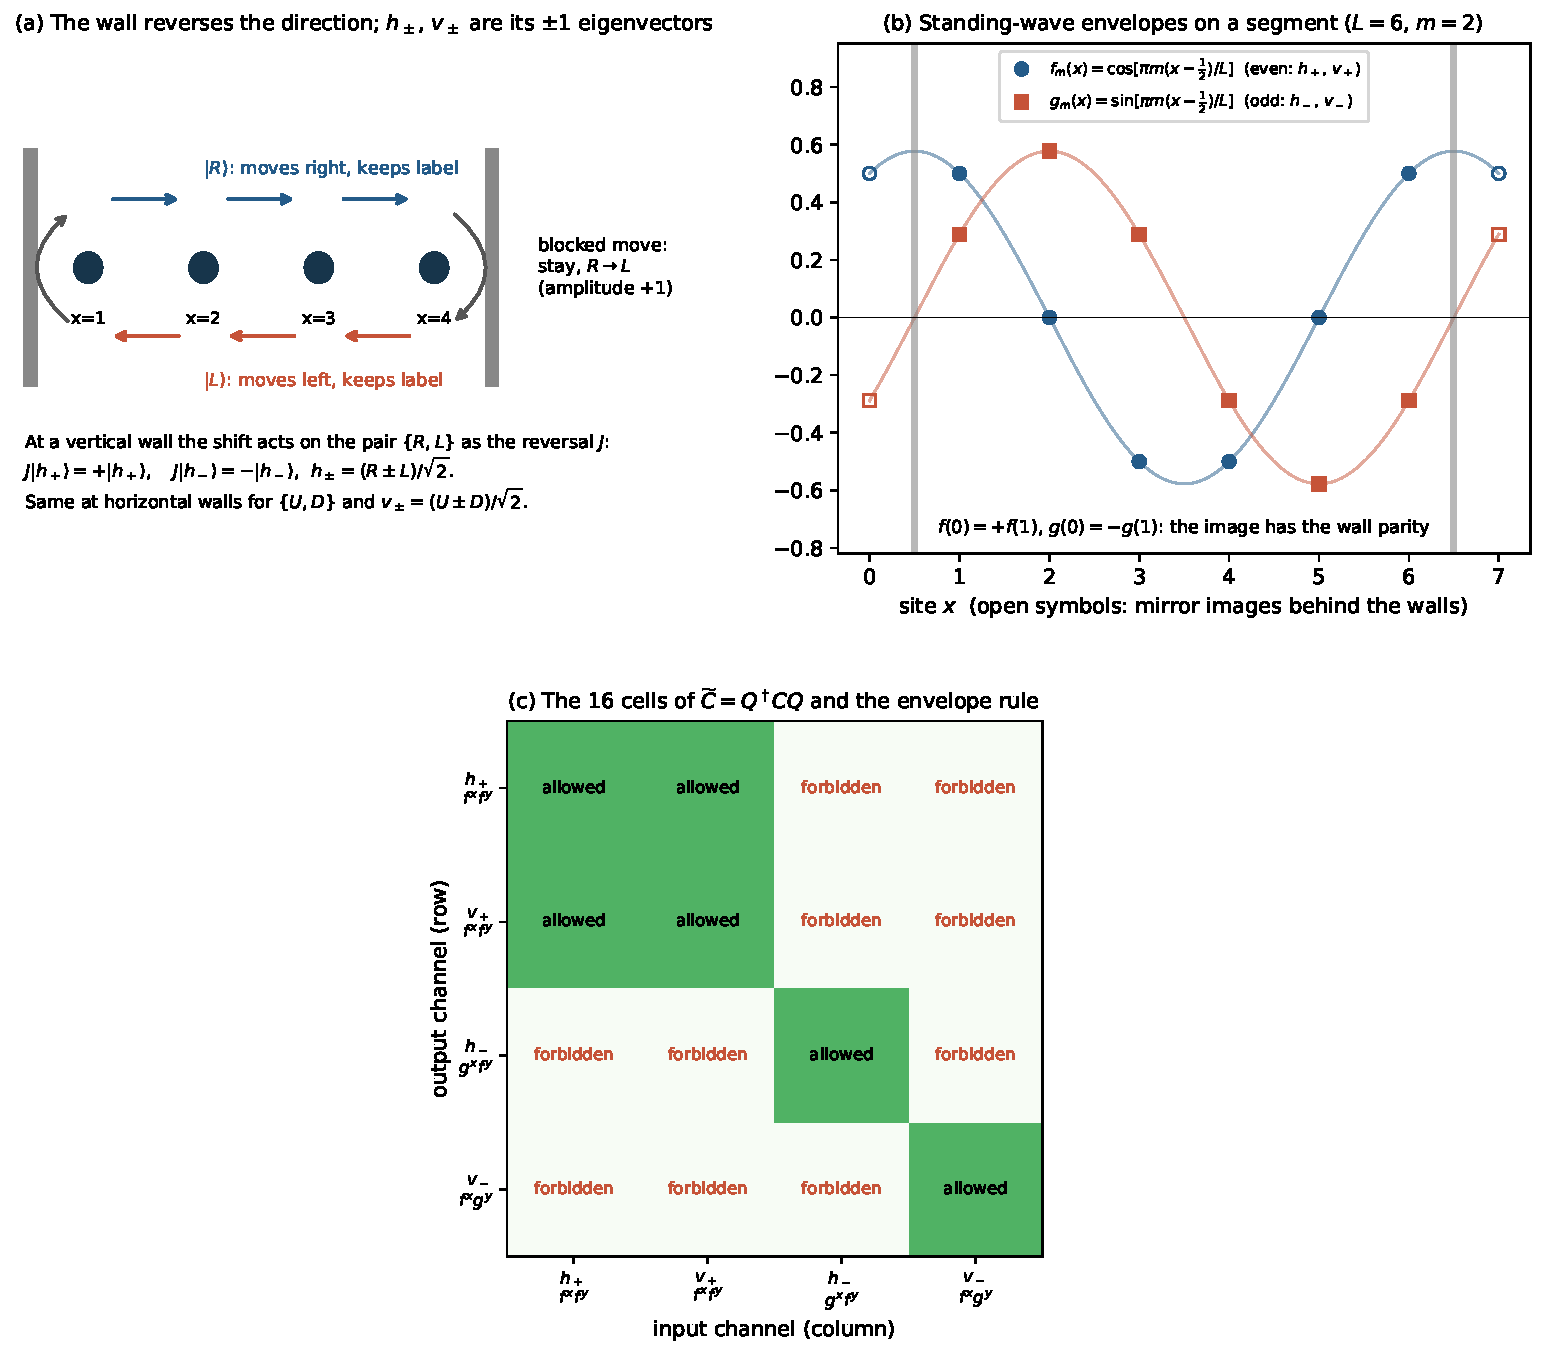
\includegraphics[width=\textwidth]{fig01_wall_envelopes_mask.pdf}
\caption{(a) A blocked move keeps the walker on its site and reverses its
direction with amplitude \(+1\). On the pair \(\{R,L\}\) this is the
exchange \(J\); its eigenvectors are the coherent channels
\(h_\pm=(R\pm L)/\sqrt2\), with eigenvalues \(\pm1\), and likewise
\(v_\pm\) for \(\{U,D\}\) at the horizontal walls.
(b) The envelope of a channel along its own axis, on a segment of six
sites (\(m=2\)). A channel with wall eigenvalue \(+1\) has a cosine
envelope \(f_m\), whose mirror value behind the wall (open symbol) has
the same sign. A channel with eigenvalue \(-1\) has a sine envelope
\(g_m\), whose mirror value has the opposite sign.
(c) The coin matrix written in the coherent basis
\((h_+,v_+,h_-,v_-)\): rows are output channels, columns are input
channels, and each label lists the envelope that the channel carries in a
standing wave. Only the six cells joining channels with the same envelope
are allowed.}
\label{fig:wallmask}
\end{figure}

\section{Two bases for the four internal states; the coherent channels}
\label{sec:panela}

So far the internal states have been written in the \emph{physical basis}
\(\{\ket R,\ket L,\ket U,\ket D\}\): each vector is a definite direction of
motion. This basis is natural for the shift in the bulk, where each
direction simply moves. At a wall it is not natural. Consider one row and
only the horizontal directions:
\begin{itemize}
\item at the right wall the blocked move sends \(\ket{N_x,y,R}\) to
\(\ket{N_x,y,L}\);
\item at the left wall it sends \(\ket{1,y,L}\) to \(\ket{1,y,R}\).
\end{itemize}
On the pair space \(\spanof\{\ket R,\ket L\}\) the wall therefore acts as
the exchange \(R\leftrightarrow L\), which is the horizontal block of the
reversal \(J\) of Chapter~\ref{ch:shift}. Neither \(\ket R\) nor
\(\ket L\) is returned as itself; each is turned into the other.

The combinations that the wall returns as themselves, up to a sign, are
the eigenvectors of the exchange. We define the four \textbf{coherent
channels}
\begin{equation}
\boxed{
\ket{h_\pm}=\frac{\ket R\pm\ket L}{\sqrt2},\qquad
\ket{v_\pm}=\frac{\ket U\pm\ket D}{\sqrt2},\qquad
J\ket{h_\pm}=\pm\ket{h_\pm},\quad J\ket{v_\pm}=\pm\ket{v_\pm}.}
\label{eq:coherentvectors}
\end{equation}
They form a second orthonormal basis of the same four-dimensional space
\(\mathbb C^4\), the \emph{coherent basis}. ``Coherent'' refers to the
fact that each channel is a superposition with fixed relative sign of two
opposite directions, rather than a single direction. The letter \(h\)
marks the horizontal pair and \(v\) the vertical pair. The sign \(\pm\) is
the channel's \textbf{wall parity}: the factor it acquires when it is
reversed at a wall.

Two properties of the moving shift will be used below.
\begin{itemize}
\item A horizontal channel moves only along \(x\), so it is blocked only
by the two vertical walls \(x=1\) and \(x=N_x\). Its wall parity
therefore constrains its spatial profile along \(x\), not along \(y\).
Likewise \(v_\pm\) feel only the horizontal walls and are constrained
only along \(y\).
\item The shift never mixes the horizontal pair with the vertical pair,
and the walls never mix a \(+\) channel with a \(-\) channel. Any such
mixing in the full walk must come from the coin.
\end{itemize}

\section{The envelope of a state}
\label{sec:envelopedef}

A general walker state assigns an amplitude \(\psi_d(\mathbf r)\) to every
site and internal state. Many important states have a simpler,
\emph{product} form: one fixed internal vector \(\ket\chi\) multiplied
by one spatial function \(F(\mathbf r)\),
\begin{equation}
\ket\Psi=\sum_{\mathbf r\in\Omega}F(\mathbf r)\ket{\mathbf r}\otimes
\ket\chi\equiv\ket F\otimes\ket\chi .
\end{equation}
We call the spatial function \(F\) the \textbf{envelope} of the state and
\(\ket\chi\) its internal state. For example,
\(\ket{f_m^xf_n^y}\otimes\ket{h_+}\) has envelope
\(F(x,y)=f_m(x)f_n(y)\) and internal state \(h_+\): at every site the
walker is in the same superposition \((R+L)/\sqrt2\), with the amplitude
modulated in space by \(F\). An envelope is defined only for product
states. A general state is a sum of such terms, each with its own
envelope and channel.

The point of this definition is that the coin and the shift treat the two
factors differently:
\begin{itemize}
\item the coin \(\Id_{\mathrm{pos}}\otimes C\) changes the internal state
and leaves the envelope untouched:
\(\ket F\otimes\ket\chi\mapsto\ket F\otimes C\ket\chi\);
\item the shift moves amplitude between sites, so it changes the
envelope. At a wall it also multiplies the channel by its wall parity.
\end{itemize}

\section{Panel (b): the wall parity fixes the envelope of each channel}
\label{sec:panelb}

Which envelopes are compatible with the walls? Consider a horizontal
channel of parity \(\pm1\) on a row of \(L=N_x\) sites. The
stay-and-reverse rule says that amplitude arriving at the wall comes back
from the same site, multiplied by the parity. This is exactly what one
obtains by continuing the envelope to a mirror site behind each wall, at
\(x=0\) and \(x=L+1\), with
\begin{itemize}
\item the \emph{same sign} for parity \(+1\): \(F(0)=F(1)\) and
\(F(L+1)=F(L)\);
\item the \emph{opposite sign} for parity \(-1\): \(F(0)=-F(1)\) and
\(F(L+1)=-F(L)\).
\end{itemize}
The mirror plane lies half a site beyond the last allowed site. The
standing waves that satisfy these conditions are the half-site-shifted
cosines \(f_m\) (parity \(+1\)) and sines \(g_m\) (parity \(-1\)) defined
precisely in Eq.~\eqref{eq:fgdef} below and drawn in
Fig.~\ref{fig:wallmask}(b). The same holds for a vertical channel along
\(y\).

Each channel's parity fixes the envelope factor along its own axis. The
factor along the other axis is fixed by the requirement, explained in
Section~\ref{sec:projectors}, that the four channels form one invariant
subspace of the shift. The result, used throughout the notes, is:
\begin{center}
\begin{tabular}{@{}llll@{}}\toprule
Coherent channel & Moves along & Wall parity & Envelope in the mode \((m,n)\)\\\midrule
\(h_+\) & \(x\) & \(+1\) & \(f_m(x)\,f_n(y)\)\\
\(v_+\) & \(y\) & \(+1\) & \(f_m(x)\,f_n(y)\)\\
\(h_-\) & \(x\) & \(-1\) & \(g_m(x)\,f_n(y)\)\\
\(v_-\) & \(y\) & \(-1\) & \(f_m(x)\,g_n(y)\)\\\bottomrule
\end{tabular}
\end{center}
Two channels share an envelope only in the case of \(h_+\) and \(v_+\).
\(h_-\) and \(v_-\) have the same parity, but their sines run along
different axes, so their envelopes differ.

\section{The standing waves of the reflecting shift}
\label{sec:standing}

Recall the coherent channels of Eq.~\eqref{eq:coherentvectors}.
On a segment of \(L\) sites define normalized profiles
\begin{align}
f_m^{(L)}(j)&=\sqrt{\frac{2-\delta_{m0}}{L}}
\cos\!\left[\frac{\pi m}{L}(j-\tfrac12)\right],
&&m=0,\ldots,L-1,\label{eq:fgdef}\\
g_m^{(L)}(j)&=\sqrt{\frac{2-\delta_{mL}}{L}}
\sin\!\left[\frac{\pi m}{L}(j-\tfrac12)\right],
&&m=1,\ldots,L.
\end{align}
Each family separately is an orthonormal basis on the \(L\) sites.
The half-site offset makes its even or odd continuation compatible
with the stay-and-reverse boundary rule.

For \(1\leq m<N_x\), with \(k_m=\pi m/N_x\), the horizontal
shift satisfies the verified identities
\begin{align}
S_x\ket{f_m^x;h_+}
&=\cos k_m\ket{f_m^x;h_+}+\sin k_m\ket{g_m^x;h_-},\\
S_x\ket{g_m^x;h_-}
&=-\sin k_m\ket{f_m^x;h_+}+\cos k_m\ket{g_m^x;h_-}.
\label{eq:moderotation}
\end{align}
Here \(f_m^x=f_m^{(N_x)}\). Trigonometric addition formulas verify
the interior relations, and the even/odd continuations verify both
endpoints. There are also endpoint modes
\begin{equation}
S_x\ket{f_0^x;h_+}=\ket{f_0^x;h_+},\qquad
S_x\ket{g_{N_x}^x;h_-}=-\ket{g_{N_x}^x;h_-}.
\end{equation}
The vertical formulas replace \(x,h,N_x,m\) by \(y,v,N_y,n\).

Equation~\eqref{eq:moderotation} says that the shift can mix a cosine
component and a sine component while preserving their common mode
index. Conservation of a mode label is not the absence of evolution.

\section{The complete mode sectors and their projectors}
\label{sec:projectors}

For \(0\leq m<N_x\), \(0\leq n<N_y\), group the following
orthonormal states:
\begin{align}
\ket{a_{mn}}&=\ket{f_m^x}\otimes\ket{f_n^y}\otimes\ket{h_+},\\
\ket{b_{mn}}&=\ket{f_m^x}\otimes\ket{f_n^y}\otimes\ket{v_+},\\
\ket{c_{mn}}&=\ket{g_m^x}\otimes\ket{f_n^y}\otimes\ket{h_-},
&&m>0,\\
\ket{d_{mn}}&=\ket{f_m^x}\otimes\ket{g_n^y}\otimes\ket{v_-},
&&n>0.
\end{align}
Their span is \(\mathcal K_{mn}\), with dimension
\(r_{mn}=2+\mathbf1_{m>0}+\mathbf1_{n>0}\). Zero-index sine terms
are omitted. The associated projector is explicitly
\begin{equation}
\boxed{
P_{mn}=\ket{a_{mn}}\bra{a_{mn}}
+\ket{b_{mn}}\bra{b_{mn}}
+\mathbf1_{m>0}\ket{c_{mn}}\bra{c_{mn}}
+\mathbf1_{n>0}\ket{d_{mn}}\bra{d_{mn}}.
}
\label{eq:pmn}
\end{equation}
Terms whose vectors are absent are simply left out of this sum.

To complete the basis, include the terminal singletons
\begin{align}
\mathcal E_n^H&=\spanof\{\ket{g_{N_x}^x f_n^y;h_-}\},
&&0\leq n<N_y,\\
\mathcal E_m^V&=\spanof\{\ket{f_m^x g_{N_y}^y;v_-}\},
&&0\leq m<N_x.
\end{align}
Their projectors are the outer products of the displayed normalized
vectors. All these spaces are mutually orthogonal and
\begin{equation}
\sum_{m,n}r_{mn}+N_x+N_y=4N_xN_y.
\end{equation}
They form a complete decomposition, denoted \(\mathscr P_{\sw}\).
The shift preserves every sector:
\begin{equation}
[S,P_a]=0\qquad(P_a\in\mathscr P_{\sw}).
\end{equation}
The index \(a\) collectively denotes \((m,n)\), \((H,n)\), or
\((V,m)\). Every \(P_a\) acts on position \emph{and} coin and has
matrix size \(D\times D\). It is not a local \(4\times4\) projector.

Each sector is the smallest shift-invariant space containing the two
symmetric states \(a_{mn},b_{mn}\): the shift rotates \(a_{mn}\) into
\(c_{mn}\) along \(x\) and \(b_{mn}\) into \(d_{mn}\) along \(y\)
(Eq.~\eqref{eq:moderotation}), never across. This is why the four
channels of one sector carry the four envelopes of
Section~\ref{sec:panelb}. These modes are constructed before selecting
\(C\) and without diagonalizing \(U\). Whether a coin preserves them is a subsequent
question. The row/column decomposition and this standing-wave
decomposition are different useful organizations of the same shift.
They need not survive the same coin.

\section{The simplest example: the identity coin}
\label{sec:identitycoin}

Before any nontrivial coin is introduced, it helps to see the cycles and
the standing waves at work in the one case where nothing else happens.
Take \(C=\Id_4\). Then
\begin{equation}
U=S(\Id_{\mathrm{pos}}\otimes\Id_4)=S:
\end{equation}
the walk \emph{is} the shift. This is the precise meaning of ``a walk
without a coin'' in this model. The four internal states are still
present, because the shift needs the direction label to know where to
move and what to reverse at a wall. What is absent is any mixing of the
directions. A walk with no internal space at all would be a different
model. A global phase, \(C=e^{i\phi}\Id_4\), is equally trivial: it only
rotates every eigenphase by \(\phi\).

\textbf{Cycles.} Since nothing mixes the directions, a walker that starts
in \(\ket{x,y,R}\) moves right along its row, is reversed at the wall,
returns as \(L\), is reversed again at the other wall, and so on
(Fig.~\ref{fig:identitycycles}(a)). Every row is one closed cycle of
\(2N_x\) basis states and every column one of \(2N_y\). A state never
leaves its cycle, so the dynamics is a set of independent
one-dimensional rotations. Fourier transformation along each cycle gives
the complete spectrum:
\begin{equation}
\spec U=\Big\{e^{i\pi k/N_x}\Big\}_{k=0}^{2N_x-1}\ \text{each }N_y\text{ times}
\ \cup\
\Big\{e^{i\pi k/N_y}\Big\}_{k=0}^{2N_y-1}\ \text{each }N_x\text{ times},
\qquad U^{2\operatorname{lcm}(N_x,N_y)}=\Id .
\label{eq:identityspectrum}
\end{equation}
\exact These are the shift cycles of Chapter~\ref{ch:rectangle}.
\session Direct diagonalization agrees with
Eq.~\eqref{eq:identityspectrum} to \(2\times10^{-15}\) on \(7\times5\)
and \(8\times6\). The smallest periods found, \(70\) and \(48\), equal
\(2\operatorname{lcm}(N_x,N_y)\). The identical copies of every row and
every column make this spectrum massively degenerate, so level
statistics are meaningless here.

\textbf{Standing waves inside a cycle.} The same dynamics can be read in
the standing-wave basis. On one row, the shift turns the cosine-envelope
state \(f_m h_+\) into the sine-envelope state \(g_m h_-\) and back, by
the angle \(\pi m/N_x\) per step (Eq.~\eqref{eq:moderotation}). The
weight never leaves this pair, as Fig.~\ref{fig:identitycycles}(c) shows.
The eigenvalues \(e^{\pm i\pi m/N_x}\) of this two-dimensional rotation,
together with \(+1\) for \(f_0h_+\) and \(-1\) for \(g_{N_x}h_-\), are
exactly the \(2N_x\) roots of unity of one row cycle. The standing waves
are therefore not something added to the shift: they are another basis
for the same cycles, one in which the wall rule is built into the
envelopes.

\textbf{Running versus standing waves.} With \(C=\Id\) the sector
\(\mathcal K_{mn}\) splits further, into an \(x\)-pair \((a_{mn},c_{mn})\)
and a \(y\)-pair \((b_{mn},d_{mn})\) that never talk to each other. The
eigenvector \((a_{mn}-ic_{mn})/\sqrt2\) of the \(x\)-pair is a wave
running around the row cycle. Its spatial density is uniform along \(x\),
because \(f_m^2+g_m^2\) is constant for a nonterminal index; only the
\(y\) standing wave survives (Fig.~\ref{fig:standingwaves}, bottom
left). A coin that couples \(h_+\) with \(v_+\), such as Grover, joins
the two pairs into one four-dimensional block. Its eigenstates then
carry a genuinely two-dimensional standing-wave pattern
(Fig.~\ref{fig:standingwaves}, bottom middle). Both displayed states were
checked to be exact eigenvectors of the full walk, with residual below
\(10^{-15}\).

In the language of the rest of this chapter, the identity coin is the
member \(C_+=\Id_2\), \(\alpha=\beta=0\) of the exactly solvable family of
Section~\ref{sec:envelope}. Its 16-cell square has weight only on the
diagonal, in allowed cells. It also belongs to the other three solvable
families of Section~\ref{sec:squarelimits}: it is monomial, it is block
diagonal by axis, and it is trivially its own gauge image. It is the most
degenerate integrable walk of the rectangle.

\begin{figure}[htbp]
\centering
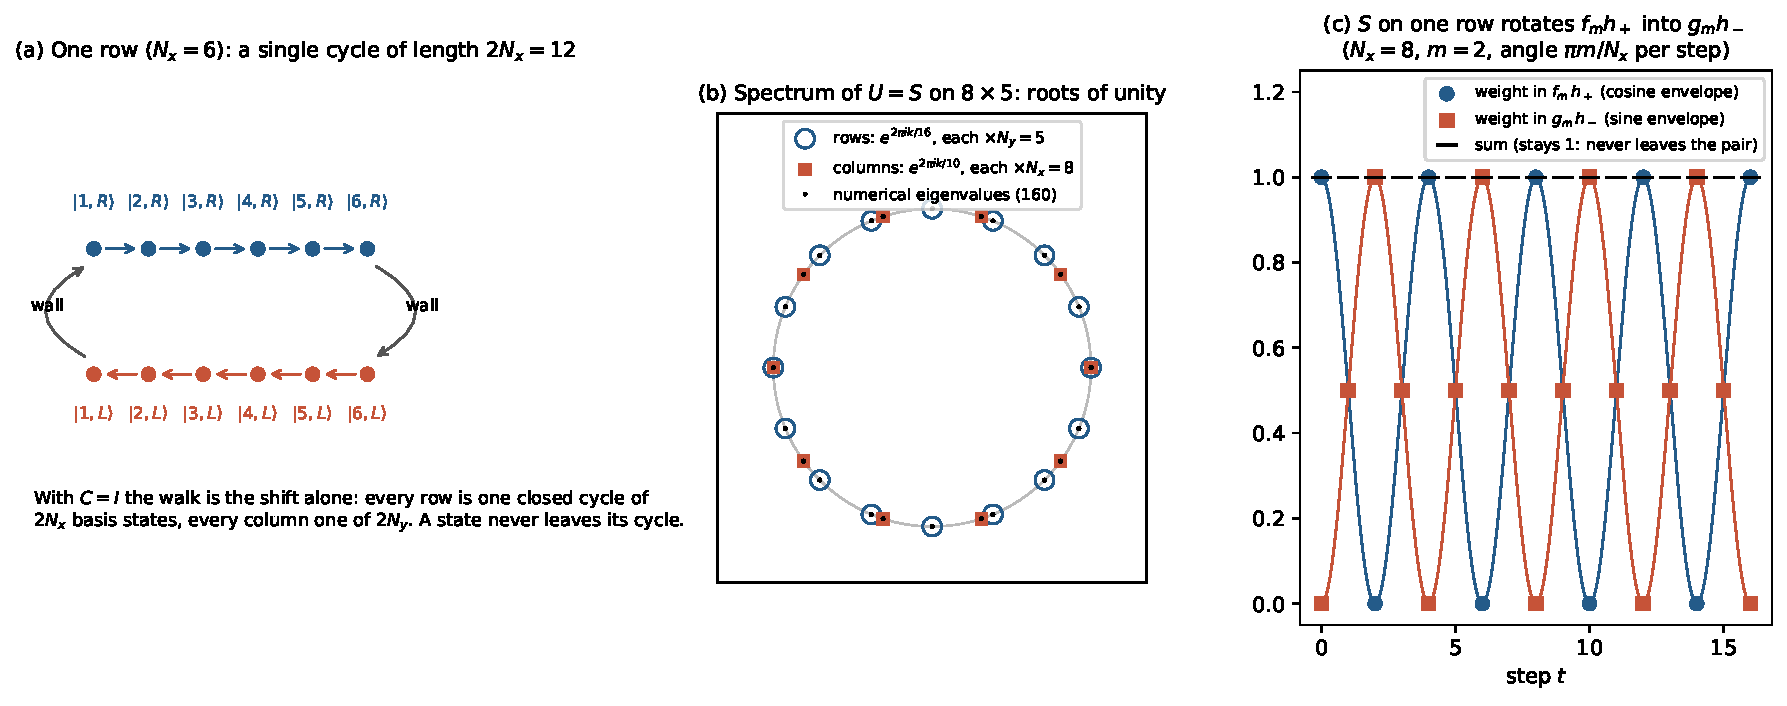
\includegraphics[width=\textwidth]{fig12_identity_coin_cycles.pdf}
\caption{The identity coin, \(U=S\).
(a) One row of six sites forms a single cycle of twelve basis states:
\(R\) states move right, the wall turns \(R\) into \(L\), \(L\) states
move left, and the other wall closes the cycle.
(b) Spectrum on \(8\times5\): the \(16\)th roots of unity from the rows,
each repeated \(N_y=5\) times, and the \(10\)th roots from the columns,
each repeated \(N_x=8\) times. Black dots are the numerically computed
eigenvalues.
(c) Starting from the cosine-envelope standing wave \(f_2h_+\) on a row
of eight sites, the shift alone rotates the weight into the sine-envelope
state \(g_2h_-\) and back, by \(\pi/4\) per step. The sum of the two
weights stays equal to one.}
\label{fig:identitycycles}
\end{figure}

\begin{figure}[htbp]
\centering
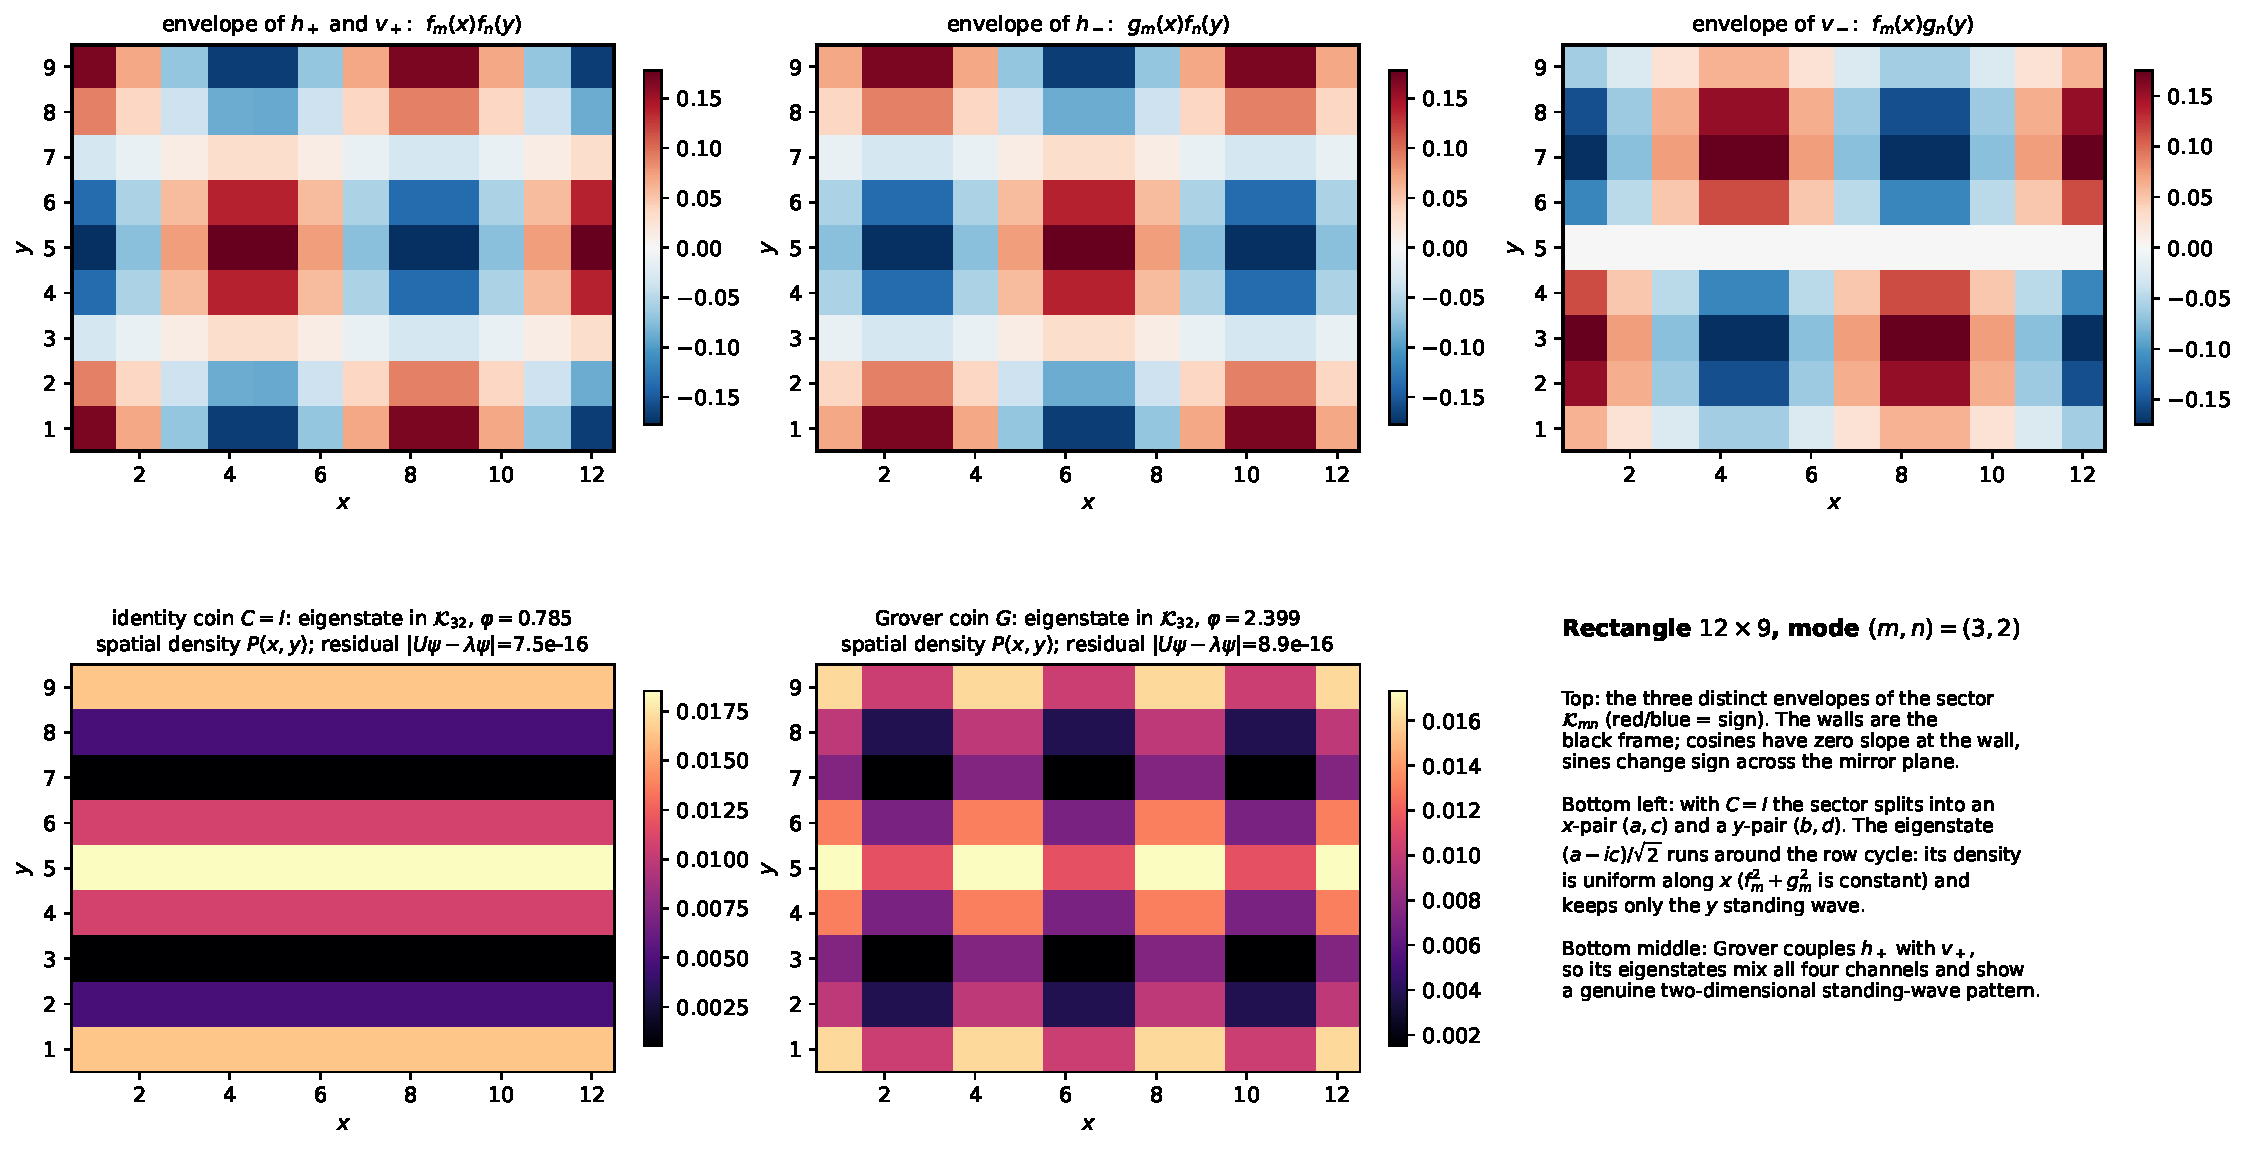
\includegraphics[width=\textwidth]{fig13_standing_waves_2D.pdf}
\caption{Standing waves on a \(12\times9\) rectangle, mode
\((m,n)=(3,2)\).
Top: the three distinct envelopes of the sector \(\mathcal K_{32}\)
(colour = value and sign). \(h_+\) and \(v_+\) share
\(f_m(x)f_n(y)\); \(h_-\) carries \(g_m(x)f_n(y)\) and \(v_-\) carries
\(f_m(x)g_n(y)\). The black frame marks the walls: a cosine factor is
flat across the mirror plane, and a sine factor changes sign across it.
Bottom: spatial density \(P(x,y)=\sum_d|\psi_d(x,y)|^2\) of one exact
eigenstate in this sector. Left, identity coin: a wave running around the
row cycle, uniform along \(x\). Middle, Grover: the four channels are
coupled and the density is a two-dimensional standing-wave pattern.}
\label{fig:standingwaves}
\end{figure}

\section{Why a \(4\times4\) square decides compatibility}
\label{sec:whysquare}

We now combine the two previous steps. Take one standing-wave state of a
sector \(\mathcal K_{mn}\): a product state with coherent channel \(j\)
and the envelope \(E_j\) that the table of Section~\ref{sec:panelb}
assigns to channel \(j\). Apply the coin. By
Section~\ref{sec:envelopedef}, the envelope is untouched and only the
internal state changes:
\begin{equation}
(\Id_{\mathrm{pos}}\otimes C)\,\ket{E_j}\otimes\ket j
=\sum_{i}\ \widetilde C_{ij}\ \ket{E_j}\otimes\ket i,\qquad
\widetilde C_{ij}=\bra iC\ket j,
\label{eq:coinonmode}
\end{equation}
where \(i,j\) run over the four coherent channels. Every output term
keeps the \emph{input's} envelope \(E_j\) but now sits in channel \(i\).
Whether the result is still inside \(\mathcal K_{mn}\) therefore depends
on only two things:
\begin{itemize}
\item the \(4\times4\) numbers \(\widetilde C_{ij}\), which say how much
amplitude goes from channel \(j\) to channel \(i\);
\item whether the envelope \(E_j\) is the one that \(\mathcal K_{mn}\)
requires for channel \(i\), that is whether \(E_i=E_j\).
\end{itemize}
The shift needs no further analysis, because it already keeps every
\(\mathcal K_{mn}\) (Section~\ref{sec:projectors}).

So the whole question reduces to a table with four inputs and four
outputs: the coin matrix itself, written as a square of
\(4\times4=16\) cells. This is the \textbf{16-cell square} used for every
coin in these notes. It is not an extra construction or an auxiliary
\(4\times4\) object: it is the coin matrix, displayed in a basis chosen to
make the envelope question readable.

\section{Which basis may be used for the square?}
\label{sec:square}

\textbf{Any orthonormal basis gives a valid square.} A \(4\times4\) unitary
can be written in any orthonormal basis \(\{\ket{e_1},\ldots,\ket{e_4}\}\)
of \(\mathbb C^4\). If the basis vectors are the columns of a unitary
matrix \(Q\), the entries are
\[
\widetilde C=Q^\dagger CQ,\qquad \widetilde C_{ij}=\bra{e_i}C\ket{e_j}.
\]
All such squares describe the same operator, with the same eigenvalues
and the same walk. In every basis the cell \((i,j)\) is the amplitude from
input \(e_j\) to output \(e_i\). Rows are outputs and columns are inputs.
Because \(C\) is unitary every column is a normalized vector, so for a
fixed input the numbers \(|\widetilde C_{ij}|^2\) are the probabilities of
the four outputs.

\textbf{Different bases answer different questions.} Two bases are used
in these notes, and Fig.~\ref{fig:readsquare} shows the Grover coin in
both:
\begin{center}\small
\begin{tabularx}{\textwidth}{@{}lYY@{}}\toprule
Basis & Columns of \(Q\) & Question answered cell by cell\\\midrule
Physical \((R,L,U,D)\) & \(Q=\Id_4\), so the square is \(C\) itself &
Does a definite direction of motion split into several directions?
(splitting measures of Chapter~\ref{ch:coins}; routing)\\
Coherent \((h_+,v_+,h_-,v_-)\) & Eq.~\eqref{eq:Qdef} &
Does the coin keep the envelopes of the standing waves?\\\bottomrule
\end{tabularx}
\end{center}

\textbf{Only the coherent basis carries the envelope rule.} The
allowed/forbidden reading of Section~\ref{sec:envelope} needs every basis
vector to have \emph{one definite envelope} in the standing-wave sectors.
The coherent channels have this property (table of
Section~\ref{sec:panelb}). The physical directions do not: in a
standing wave the amplitude on \(R\) is a sum of an \(h_+\) part with a
cosine envelope and an \(h_-\) part with a sine envelope. A physical-basis
cell therefore mixes allowed and forbidden contributions and cannot be
labeled either way. The mask of Fig.~\ref{fig:wallmask}(c) applies to the
coherent square only.

\textbf{What may still be chosen freely.}
\begin{itemize}
\item \emph{The order of the four channels.} We use
\((h_+,v_+,h_-,v_-)\) because it makes the allowed cells a single
\(2\times2\) block followed by two diagonal cells. Another order permutes
rows and columns together and moves the allowed cells, but does not
change which pairs are allowed.
\item \emph{Phases of the basis vectors.} These also leave the envelope
rule unchanged.
\end{itemize}
Changing the coin itself by phases, \(C\to DCD\), is a different
operation, a \emph{gauge transformation} of the walk. It is discussed in
Section~\ref{sec:squarelimits}.

With the coherent channels as columns, in the physical order
\((R,L,U,D)\),
\begin{equation}
Q=\frac1{\sqrt2}\begin{pmatrix}
1&0&1&0\\1&0&-1&0\\0&1&0&1\\0&1&0&-1
\end{pmatrix},\qquad\widetilde C=Q^\dagger C Q .
\label{eq:Qdef}
\end{equation}
For Grover, Fig.~\ref{fig:readsquare} shows that the two squares look
completely different. Every physical cell has modulus \(1/2\): each
direction splits into all four. The coherent square is a signed
permutation: \(h_+\leftrightarrow v_+\), \(h_-\to-h_-\), \(v_-\to-v_-\).
Equal probabilities in the physical square can hide a very sparse
coherent square, because the relative phases matter.

\begin{figure}[htbp]
\centering
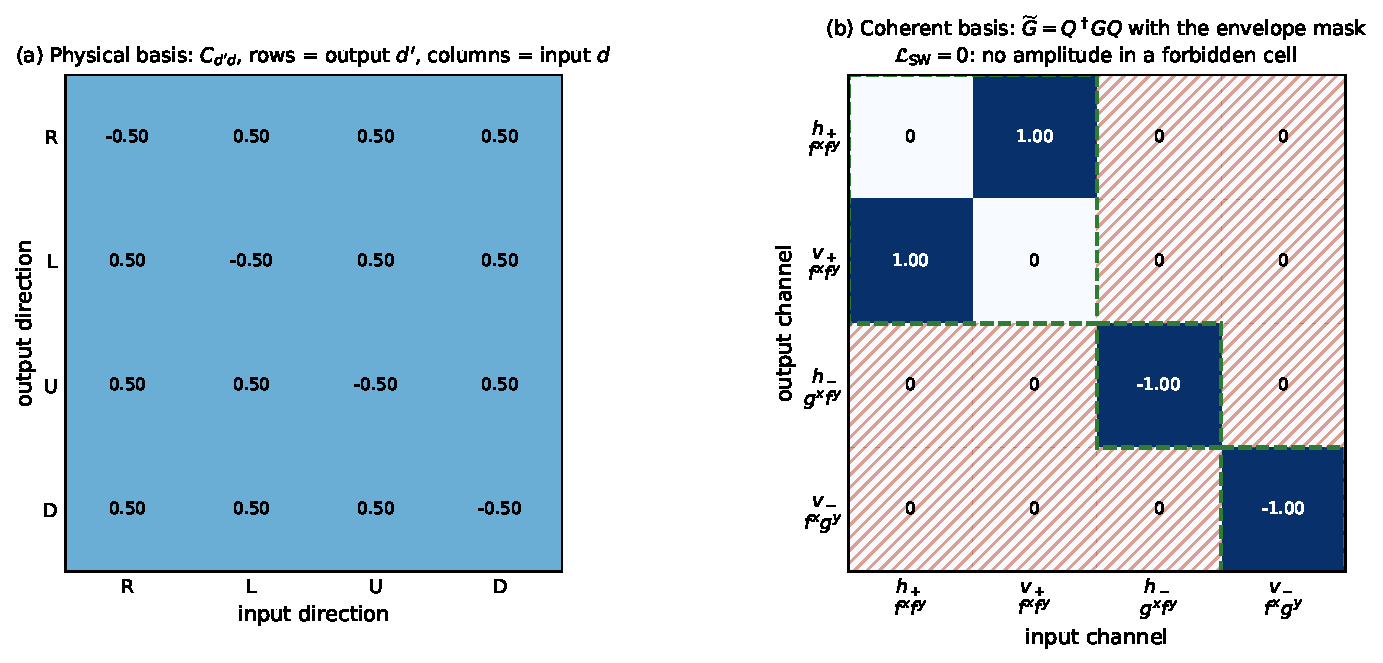
\includegraphics[width=.92\textwidth]{fig02_reading_the_square_grover.pdf}
\caption{The Grover coin as a 16-cell square in two bases.
(a) Physical basis \((R,L,U,D)\): the cell in row \(d'\) and column \(d\)
is \(C_{d'd}\), the amplitude from input direction \(d\) to output
direction \(d'\); colour is its modulus. No envelope mask applies in this
basis.
(b) Coherent basis \((h_+,v_+,h_-,v_-)\): the cell in row \(i\) and column
\(j\) is \(\widetilde G_{ij}=\bra iG\ket j\). The envelope mask is
superimposed: hatched cells are forbidden, and the dashed green boxes are
the allowed \(2+1+1\) blocks. Grover puts no amplitude in a forbidden
cell.}
\label{fig:readsquare}
\end{figure}

\section{Panel (c): allowed and forbidden cells}
\label{sec:envelope}

\textbf{The rule.} By Eq.~\eqref{eq:coinonmode}, the amplitude
\(\widetilde C_{ij}\) keeps the input's envelope \(E_j\) while moving it
to channel \(i\). It stays inside the sector \(\mathcal K_{mn}\) exactly
when \(E_i=E_j\). Otherwise it is orthogonal to the channel-\(i\) state of
the sector, because \(\langle f_m,g_m\rangle=0\) for every nonterminal
index, and it leaves \(\mathcal K_{mn}\).

\textbf{The sixteen cells.} Reading the envelopes from the table of
Section~\ref{sec:panelb}:
\begin{itemize}
\item \emph{allowed} (6 cells):
\begin{itemize}
\item the \(2\times2\) block \(\{h_+,v_+\}\to\{h_+,v_+\}\), since both
channels carry \(f_mf_n\);
\item the diagonal cells \(h_-\to h_-\) and \(v_-\to v_-\);
\end{itemize}
\item \emph{forbidden} (10 cells):
\begin{itemize}
\item the eight cells that change the wall parity
(\(+\leftrightarrow-\));
\item the two cells \(h_-\leftrightarrow v_-\), which keep the parity but
exchange the envelope \(g_mf_n\) for \(f_mg_n\).
\end{itemize}
\end{itemize}
In the order \((h_+,v_+,h_-,v_-)\) the allowed cells form the
block-diagonal pattern \(2+1+1\) of Fig.~\ref{fig:wallmask}(c).

\textbf{One number per square.} The forbidden weight is
\begin{equation}
\boxed{\mathcal L_{\sw}(C)=\frac14\sum_{(i,j)\ \mathrm{forbidden}}
|\widetilde C_{ij}|^2
=1-\frac14\Big(\sum_{a,b=1}^2|\widetilde C_{ab}|^2
+|\widetilde C_{33}|^2+|\widetilde C_{44}|^2\Big).}
\label{eq:Lswcells}
\end{equation}
\begin{itemize}
\item For each input channel \(j\), the sum of \(|\widetilde C_{ij}|^2\)
over its forbidden cells is the probability that the coin sends that
channel out of its standing-wave sector.
\item The factor \(1/4\) averages over the four input channels.
\item Since the shift keeps every sector, \(\mathcal L_{\sw}\) equals the
mean probability per step that the full walk leaves the standing-wave
sectors. This is the exact full-space identity of
Section~\ref{sec:modeleakage}, Eq.~\eqref{eq:closedleak}.
\end{itemize}

\textbf{The exactly solvable family.} \(\mathcal L_{\sw}=0\) holds if and
only if all forbidden cells vanish, that is, if the coherent square is
block diagonal:
\begin{equation}
\widetilde C=C_+\oplus e^{i\alpha}\oplus e^{i\beta},\qquad C_+\in U(2).
\end{equation}
Then every \(\mathcal K_{mn}\) is invariant under the full walk, which is
solved by blocks of dimension at most four. Combining the shift rotation
\eqref{eq:moderotation} with the coin, the restricted step in the order
\((a_{mn},b_{mn},c_{mn},d_{mn})\) is, for \(m,n>0\),
\begin{equation}
\boxed{U_{mn}=S_{mn}\,\big(C_+\oplus e^{i\alpha}\oplus e^{i\beta}\big),
\qquad
S_{mn}=\begin{pmatrix}
c_x&0&-s_x&0\\0&c_y&0&-s_y\\s_x&0&c_x&0\\0&s_y&0&c_y
\end{pmatrix},}
\label{eq:generalblock}
\end{equation}
with \(c_x=\cos(\pi m/N_x)\), \(s_x=\sin(\pi m/N_x)\), and similarly
\(c_y,s_y\). Rows and columns of absent vectors are deleted when \(m=0\)
or \(n=0\), and at \((0,0)\) the block is \(C_+\) itself. The \(N_y\)
horizontal terminal singletons have eigenvalue \(-e^{i\alpha}\), and the
\(N_x\) vertical ones have eigenvalue \(-e^{i\beta}\).

For \(C_+=\sigma_x\) and \(\alpha=\beta=\pi\) this reproduces the Grover
blocks of Section~\ref{sec:groverfull}. In a numerical check for this
revision, the union of these block spectra matched direct diagonalization
of the full walk to \(4.6\times10^{-15}\) on \(7\times5\) and
\(7.8\times10^{-15}\) on \(8\times6\). After a gauge transformation, the
same formula also gives the compass Fourier walk
(Section~\ref{sec:fourierfull}).

\section{What the square can and cannot decide}
\label{sec:squarelimits}

The mask tests one family of geometric modes. A zero forbidden weight is
\emph{sufficient} for an exact block solution. A nonzero weight is not a
proof of non-integrability, for three demonstrated reasons, each with its
own fingerprint in the squares.
\begin{itemize}
\item \textbf{Gauge.} The walks built from \(C\) and from
\(DCD\), \(D=\diag(e^{ia},e^{-ia},e^{ib},e^{-ib})\), are unitarily
equivalent (Appendix~\ref{app:gauge}). The equivalence maps the standing
waves onto phase-modulated versions of themselves, so a coin may fill
forbidden cells while its gauge image does not. The gauge-adjusted test
is
\(\mathcal L^*_{\sw}=\min_D\mathcal L_{\sw}(DCD)\).
\item \textbf{Routing.} A monomial coin, with one nonzero cell per column
of the \emph{physical} square, is solved by deterministic cycles whatever
its coherent square looks like.
\item \textbf{Independent axes.} A coin that never mixes \(\{R,L\}\) with
\(\{U,D\}\) is solved row by row and column by column.
\end{itemize}
\begin{center}\small
\begin{tabularx}{\textwidth}{@{}lYY@{}}\toprule
Reduction family & Fingerprint & Example\\\midrule
Fixed standing waves & Coherent square: no weight in forbidden cells
& Grover \(G\)\\
Gauge images of standing waves & Coherent square of \(DCD\): no weight in forbidden cells
& Compass Fourier \(F_c\): \(\mathcal L_{\sw}=\tfrac12\), \(\mathcal L^*_{\sw}=0\)\\
Deterministic routing & Physical square: one nonzero cell per column
& Permutation \(P\): \(\mathcal L_{\sw}=\mathcal L^*_{\sw}=\tfrac12\)\\
Independent rows and columns & Physical square block diagonal in
\(\{R,L\}\mid\{U,D\}\); coherent square block diagonal in
\(\{h_+,h_-\}\mid\{v_+,v_-\}\) & \(C_H\oplus C_V\), e.g.\ Hadamard per axis\\\bottomrule
\end{tabularx}
\end{center}
The table also shows why both bases are needed. Two of the
fingerprints are read in the coherent basis and two in the physical
basis. These four families have not been proved exhaustive, so a coin
outside all of them still has an open status.

\section{What can already be said about coin compatibility?}

If \(\mathcal G\) is one of the geometric operations commuting
with \(S\), then
\begin{equation}
[U,\mathcal G]=S[\CC,\mathcal G].
\label{eq:inherit}
\end{equation}
For a homogeneous coin, the only remaining test is its commutator
with the direction permutation in \(\mathcal G\). In particular,
\begin{center}
\begin{tabular}{@{}ll@{}}
\toprule
Condition on the coin&Surviving full-walk geometric symmetry\\
\midrule
\([C,\sigma_x]=0\)&\(\mathcal P_x\)\\
\([C,\sigma_y]=0\)&\(\mathcal P_y\)\\
\([C,J]=0\)&\(\mathcal R\)\\
\([C,\tau]=0\), on a square&Diagonal reflection\\
\bottomrule
\end{tabular}
\end{center}
Likewise, because each mode projector commutes with \(S\),
\begin{equation}
[U,P_a]=0\quad\Longleftrightarrow\quad[\CC,P_a]=0.
\end{equation}
This is the bridge to the coin: the geometry supplies candidate
structures, and the coin determines which remain conserved.

\begin{lesson}{The rectangle supplies several levels of structure}
The shift has individual row/column cycles, geometric reflection
parities, and complete standing-wave sectors. These are different
labels. A coin may destroy one decomposition while preserving another.
The rectangle alone does not determine the symmetries or solvability
of the full Floquet operator.
\end{lesson}


\section{Inventory before the coin is introduced}

\begin{center}\small
\begin{tabularx}{\textwidth}{@{}lYY@{}}\toprule
Structure & Established for the shift & Question left for the coin\\\midrule
Row and column projectors & Independent cycles of lengths \(2N_x,2N_y\)
& Does it remain within each axis?\\
Geometric operations & \(\mathcal P_x,\mathcal P_y,\mathcal R\) commute with \(S\)
& Does it commute with their direction permutations?\\
Standing-wave projectors & Each explicit sector is invariant
& Does it keep coin vectors and spatial envelopes compatible?\\
16-cell coherent square & Allowed cells fixed by wall parity and envelope
& How much weight does the coin put in the ten forbidden cells?\\
Reversing operations & They turn \(S\) into \(S^{-1}\)
& Does the transpose condition hold for full-walk time reversal?\\\bottomrule
\end{tabularx}
\end{center}
These are distinct structures; the geometric group is not asserted to
exhaust the shift's commutant. The existing advanced constructions,
including uniform and checkerboard subspaces, are retained in
Appendix~\ref{app:advanced}.

\chapter{The coins as local four-dimensional operators}
\label{ch:coins}

\section{How the coins are displayed}

Every coin is given as an explicit matrix in the physical order
\((R,L,U,D)\) and then redrawn as its 16-cell coherent square
\(\widetilde C=Q^\dagger CQ\) with the envelope mask of
Chapter~\ref{ch:sixteen}. Figure~\ref{fig:basecoins} collects the
unperturbed coins and Fig.~\ref{fig:deformedcoins} the two deformed
families. The numbers in the panel titles are the fixed-mode forbidden
weight \(\mathcal L_{\sw}\) and, where computed, its gauge minimum
\(\mathcal L^*_{\sw}\). A block in the local matrix does not by itself
preserve a full-space mode projector; the full walks are examined in
Chapter~\ref{ch:assembled}.

\begin{figure}[p]
\centering
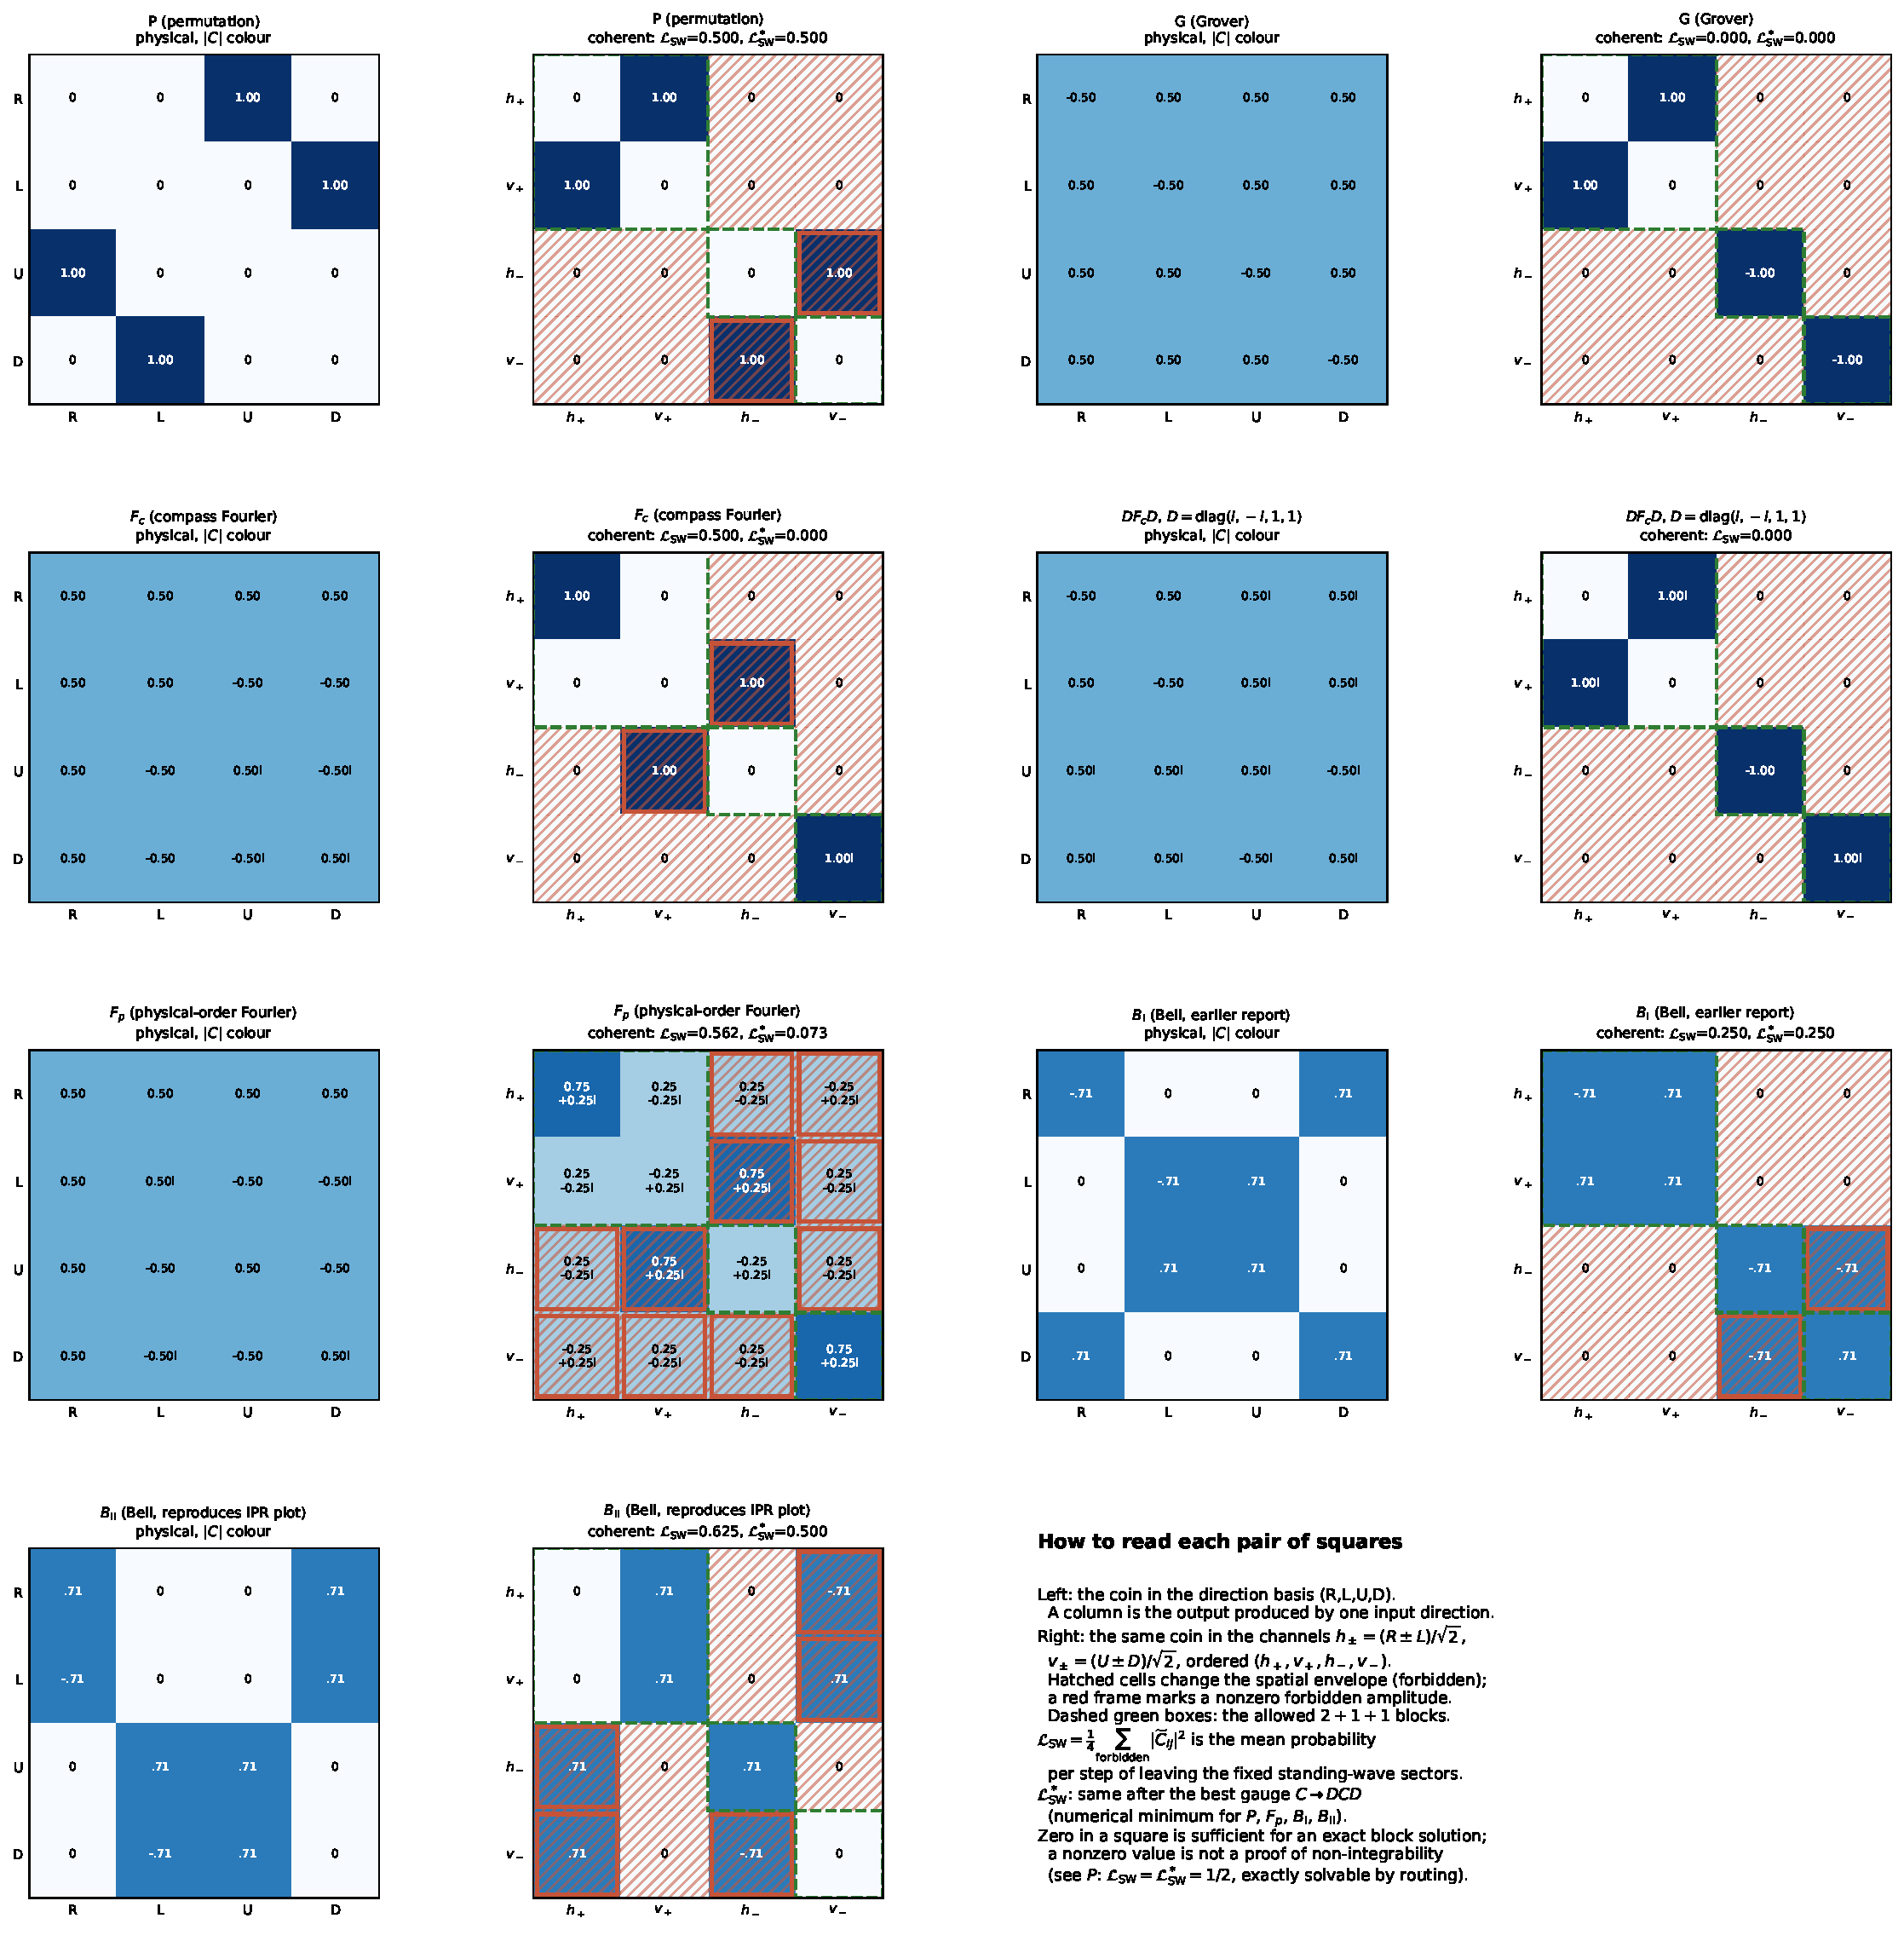
\includegraphics[width=\textwidth]{fig03_base_coins_16cells.pdf}
\caption{The unperturbed coins, each as a physical square (left of each
pair) and as a coherent square with the envelope mask (right). Red frames
mark nonzero amplitude in a forbidden cell. \(DF_cD\) is the gauge image
of the compass Fourier coin with \(D=\diag(i,-i,1,1)\): its forbidden
cells are empty. \(\mathcal L^*_{\sw}\) is exact for \(G\) and \(F_c\)
(zero) and a numerical minimum (an upper bound) for \(P\), \(F_p\),
\(B_{\mathrm I}\) and \(B_{\mathrm{II}}\).}
\label{fig:basecoins}
\end{figure}

\begin{figure}[htbp]
\centering
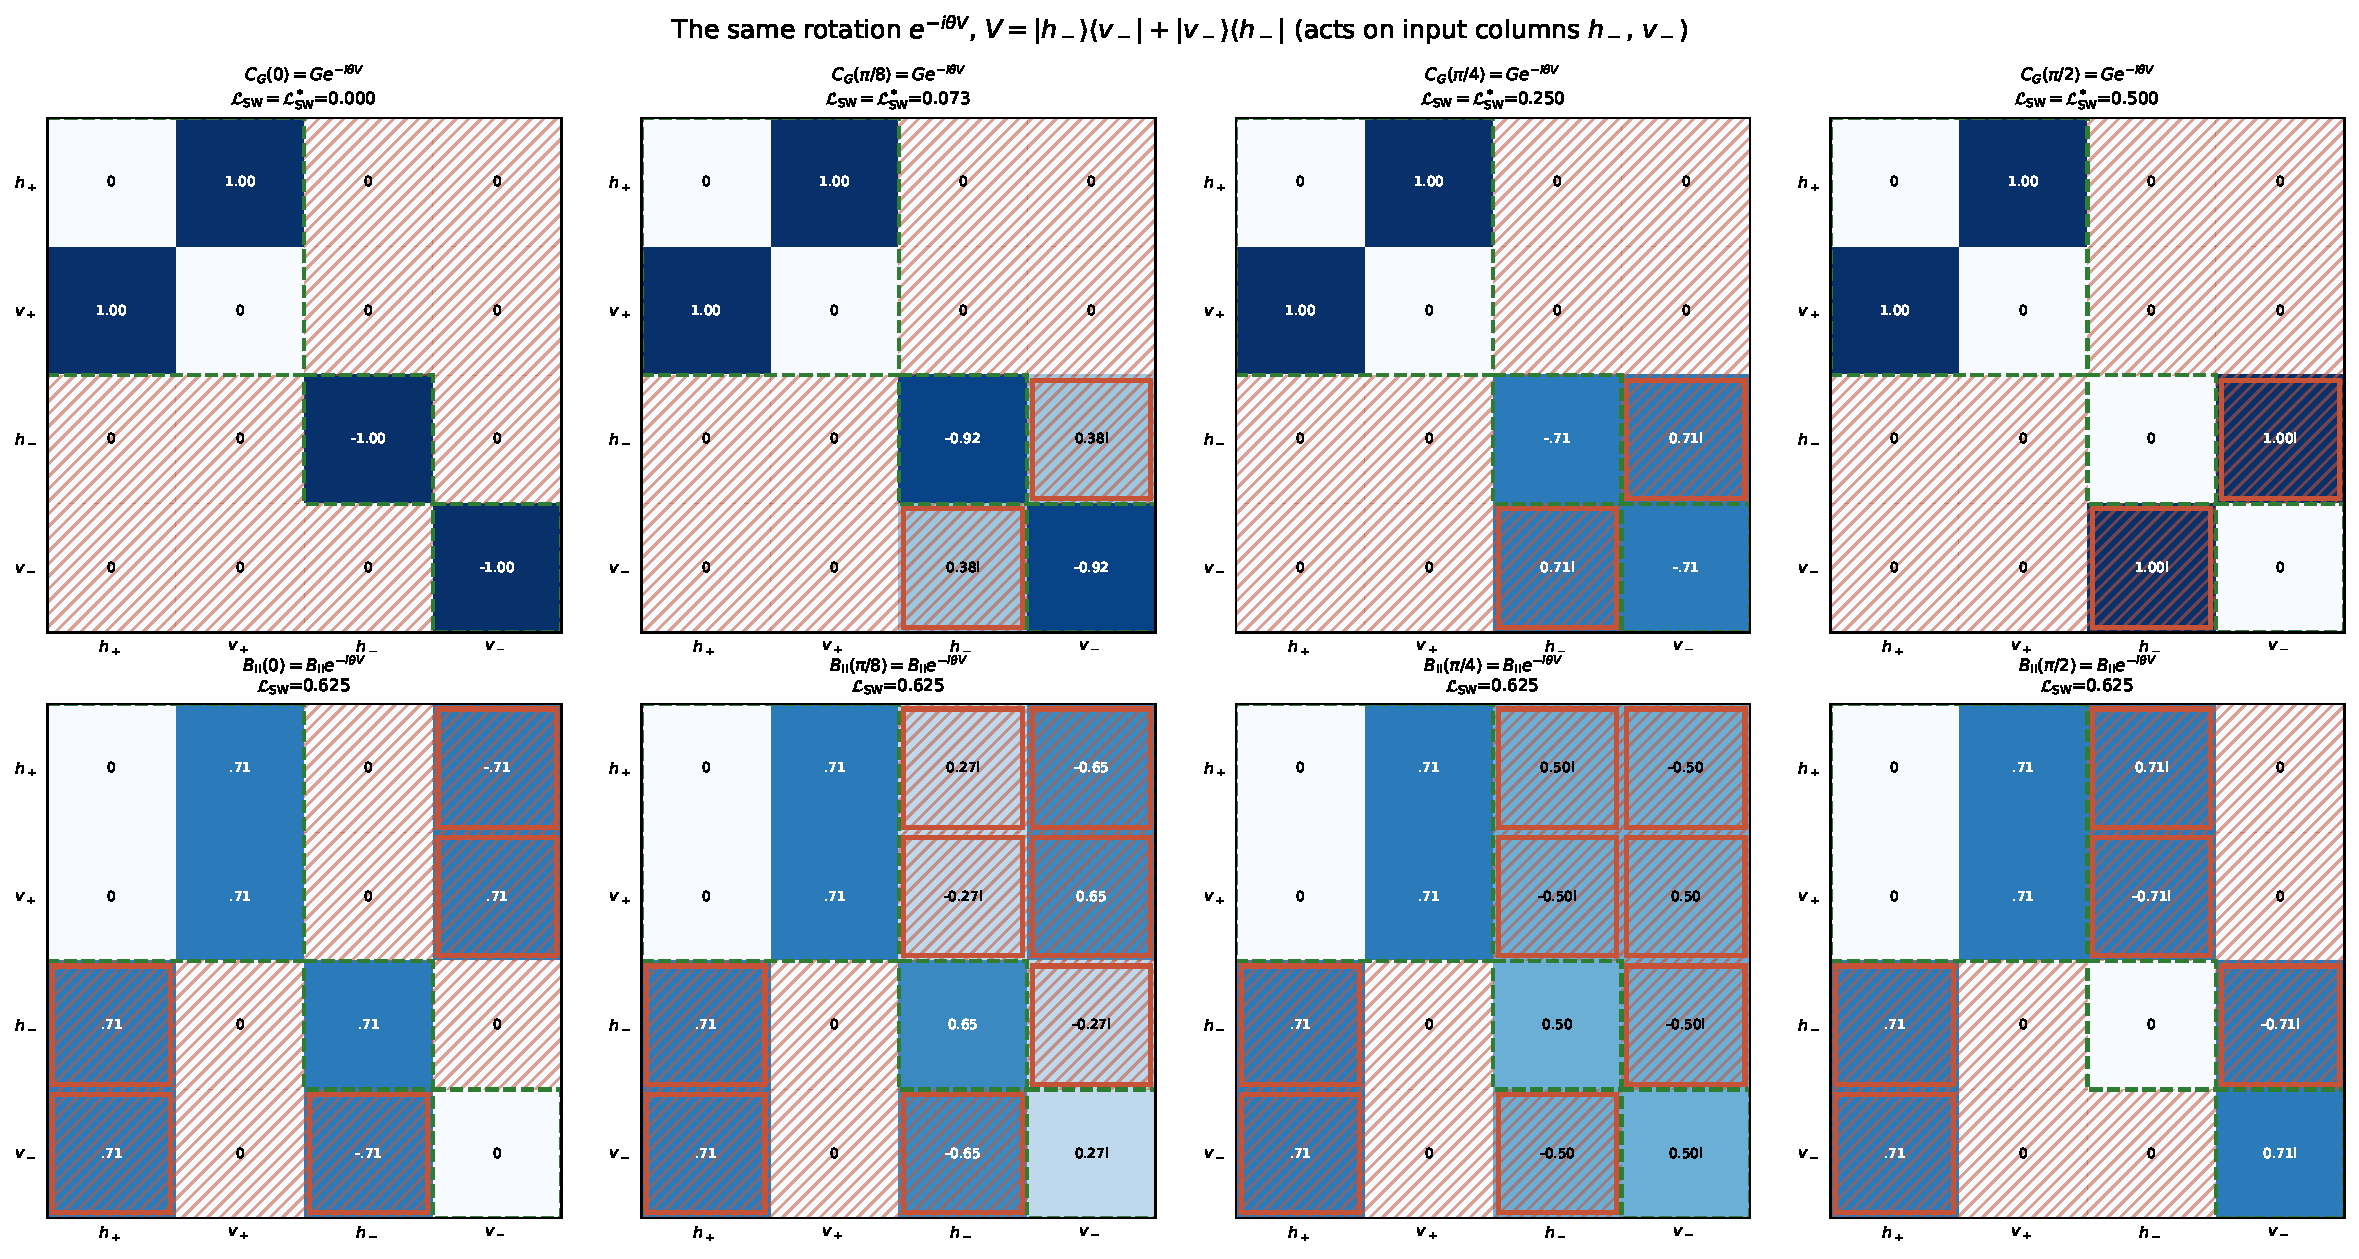
\includegraphics[width=\textwidth]{fig04_deformed_coins_16cells.pdf}
\caption{The same rotation \(e^{-i\theta V}\) applied to Grover (top) and
to \(B_{\mathrm{II}}\) (bottom), at \(\theta=0,\pi/8,\pi/4,\pi/2\).
Right multiplication acts on the input \emph{columns} \(h_-,v_-\) only.
For Grover it moves weight from the allowed diagonal cells
\((h_-,h_-),(v_-,v_-)\) into the forbidden cells \((h_-,v_-),(v_-,h_-)\);
for \(B_{\mathrm{II}}\) it only redistributes weight that was already
partly forbidden, and \(\mathcal L_{\sw}=5/8\) for every \(\theta\)
(Section~\ref{sec:modbell}).}
\label{fig:deformedcoins}
\end{figure}

\section{Three questions that a ``mixing measure'' can ask}

The physical direction basis is fixed. For a definite input direction
\(d\), the probability to obtain \(d'\) after the coin is
\begin{equation}
p(d'|d)=|C_{d'd}|^2.
\end{equation}
These probabilities do not contain the relative phases of the
amplitudes. Two distinct questions are whether an \emph{individual
direction splits} and whether a \emph{pair label is redistributed}.
A third question, coupling between spatial modes of the full walk,
will be addressed in Chapter~\ref{ch:assembled}.

\subsection{Individual-direction splitting}

The normalized output entropy, averaged over the four definite input
directions, is
\begin{equation}
\boxed{
\mathcal M_{\mathrm{split}}(C)
=-\frac1{4\ln4}\sum_{d,d'}|C_{d'd}|^2\ln|C_{d'd}|^2.
}
\label{eq:split}
\end{equation}
Use \(0\ln0=0\). It lies in \([0,1]\). It is zero exactly when
each column has a single nonzero entry. Unitarity then forces a
permutation with phases, called a \emph{monomial} coin. It equals
one when every column has four probabilities \(1/4\).

A second diagnostic, already used in the project, is
\begin{equation}
\mathcal L_{\mathrm{route}}(C)
=1-\frac14\max_{\pi\in S_4}\sum_d|C_{\pi(d),d}|^2.
\end{equation}
It measures departure from the best deterministic routing. Its zero
has the same monomial condition, although its nonzero values use a
different scale from the entropy.

\subsection{Mixing a specified pair label}

There are three unordered partitions of four directions into two pairs:
\begin{align}
q_1&=\diag(1,1,-1,-1),&\{R,L\}&\mid\{U,D\},\\
q_2&=\diag(1,-1,1,-1),&\{R,U\}&\mid\{L,D\},\\
q_3&=\diag(1,-1,-1,1),&\{R,D\}&\mid\{L,U\}.
\end{align}
For a pair \(A\),
\begin{equation}
q_A=\sum_{d\in A}\ket d\bra d-\sum_{d\notin A}\ket d\bra d.
\end{equation}
It assigns signs rather than exchanging directions:
\(q_A=q_A^\dagger\), \(q_A^2=\Id_4\), \(\Tr q_A=0\).
Its two eigenspaces identify the groups, and reversing its sign gives
the same unordered split. The original project definition is
\begin{equation}
\boxed{
\mathcal M_q(C)=\frac18\min\{
\norm{[C,q]}_F^2,\norm{\{C,q\}}_F^2\}.
}
\end{equation}
The Frobenius norm is \(\norm A_F^2=\Tr(A^\dagger A)\), and
\(\{C,q\}=Cq+qC\). A zero means the coin preserves \emph{or}
swaps these two groups. It does not mean each individual direction
remains unsplit.

For \(P_\pm=(\Id\pm q)/2\), the transition probabilities for
inputs \(P_\pm/2\) form
\begin{equation}
T_q=\frac12
\begin{pmatrix}
\norm{P_+CP_+}_F^2&\norm{P_+CP_-}_F^2\\
\norm{P_-CP_+}_F^2&\norm{P_-CP_-}_F^2
\end{pmatrix}
=\begin{pmatrix}p&1-p\\1-p&p\end{pmatrix}.
\end{equation}
The special symmetric form follows from unitarity and the equal ranks
of the groups. Explicitly, \(p=\tfrac12\norm{P_+CP_+}_F^2\). Equivalently,
\begin{equation}
\norm{[C,q]}_F^2=16(1-p),\qquad
\norm{\{C,q\}}_F^2=16p
\end{equation}
These norm formulas make the normalization explicit: when both outputs have probability
\(1/2\), the two squared norms are eight and the score is one.
Exact preservation has \(p=1\); exact swapping has \(p=0\); both
give zero, so \(\mathcal M_q=2\min(p,1-p)\).
The input here is an equal incoherent mixture inside one
pair, not every individual pure direction state. This is why a
deterministic permutation can have a nonzero pair score.

The two summaries
\begin{equation}
\mathcal M_{\mathrm{dir}}=\min_{\alpha=1,2,3}\mathcal M_{q_\alpha},
\qquad
\overline{\mathcal M}=\frac13\sum_{\alpha=1}^3\mathcal M_{q_\alpha}
\end{equation}
answer different questions. A zero of the minimum asserts that at
least one of the three pair partitions is preserved or swapped.

\subsection{The 24 permutations versus the three pair labels}

A permutation satisfies \(P_\pi\ket d=\ket{\pi(d)}\).
There are \(4!=24\) relabelings but only \(\binom42/2=3\)
unordered splits into two pairs:
\[
P_\pi q_A P_\pi^\dagger=q_{\pi(A)}.
\]
The permutations rearrange the partitions. The \(q_\alpha\) are
observables used to test pair preservation or swapping, not a list
of asserted coin symmetries. Grover's 24 equations
\(P_\pi G P_\pi^\dagger=G\) express invariance under relabeling;
they do not imply zero \(\mathcal M_q\).
A permutation matrix can also be chosen as the coin itself, a different
role from testing the symmetry of another coin.

\subsection{The proposed horizontal/vertical entropy}

Write \(C=\left(\begin{smallmatrix}C_{HH}&C_{HV}\\
C_{VH}&C_{VV}\end{smallmatrix}\right)\), grouping \(R,L\) and
\(U,D\). With the standard norm \(\norm C_F^2=4\), define
\begin{equation}
p=\frac{\norm{C_{HH}}_F^2+\norm{C_{VV}}_F^2}{4},\qquad
\mathcal M_{\mathrm{axis}}=h_2(p)
=-\frac{p\ln p+(1-p)\ln(1-p)}{\ln2}.
\end{equation}
This is a valid entropy for the axis output conditioned on the
coarse axis input, with an incoherent uniform state inside each group.
It is an entropy version of the original \(q_1\) test:
\begin{equation}
\boxed{\mathcal M_{\mathrm{axis}}
=h_2(\mathcal M_{q_1}/2).}
\end{equation}
It introduces no new zero condition. Always retaining the axis and
always swapping it both give zero.

For example, the permutation exchanging \(L,U\) and fixing \(R,D\)
has \(p=1/2\) and maximal axis entropy, although no input direction
splits. This does not invalidate the entropy; it identifies the
coarse question it answers.

\section{The identity coin}
\label{sec:identitylocal}

The trivial coin \(C=\Id_4\) is the reference point for all others. In
every basis its square is the identity, so no direction splits and no
channel changes:
\begin{equation}
\mathcal M_{\mathrm{split}}=0,\qquad
(\mathcal M_{q_1},\mathcal M_{q_2},\mathcal M_{q_3})=(0,0,0),\qquad
\mathcal L_{\sw}=\mathcal L^*_{\sw}=0,\qquad [\Id,J]=0 .
\end{equation}
Its full walk is the shift itself, whose cycles, spectrum and standing
waves were made explicit in Section~\ref{sec:identitycoin}. Every other
coin in this chapter can be read as a specific way of mixing the
otherwise independent row and column cycles.

\section{One explicit permutation coin}

Take
\begin{equation}
\boxed{
P=\begin{pmatrix}
0&0&1&0\\0&0&0&1\\1&0&0&0\\0&1&0&0
\end{pmatrix},
\qquad R\leftrightarrow U,\quad L\leftrightarrow D.
}
\end{equation}
It is a real symmetric unitary with \(P^2=\Id\) and \([P,J]=0\).
Every input direction has a unique output, so
\begin{equation}
\mathcal M_{\mathrm{split}}(P)=\mathcal L_{\mathrm{route}}(P)=0.
\end{equation}
For this particular permutation all three \(\mathcal M_q\)'s are
zero. That is not true for every permutation, as the previous
counterexample illustrates. In the coherent basis,
\begin{equation}
P:\quad h_+\leftrightarrow v_+,\qquad h_-\leftrightarrow v_-.
\end{equation}
The axis changes, but no amplitude is divided between outputs.

\section{The Grover coin}

Define \(\ket{s}=(1,1,1,1)^{\mathsf T}/2\). The Grover coin is
\begin{equation}
\boxed{
G=2\ket{s}\bra{s}-\Id
=\frac12\begin{pmatrix}
-1&1&1&1\\1&-1&1&1\\1&1&-1&1\\1&1&1&-1
\end{pmatrix}.
}
\end{equation}
It is real, symmetric, Hermitian, and unitary, with \(G^2=\Id\).
It has eigenvalue \(+1\) on \(\ket{s}\) and \(-1\) on its
three-dimensional orthogonal complement. Every direction permutation
leaves it unchanged. This is a symmetry of the \emph{coin}; only
permutations compatible with the shift and geometry can become
symmetries of the full walk.

Its probabilities are uniformly \(1/4\), giving
\begin{equation}
\mathcal M_{\mathrm{split}}(G)=1,\qquad
(\mathcal M_{q_1},\mathcal M_{q_2},\mathcal M_{q_3})(G)=(1,1,1).
\end{equation}
Its coherent action is much more restricted:
\begin{equation}
G h_+=v_+,\qquad Gv_+=h_+,\qquad
Gh_-=-h_-,\qquad Gv_-=-v_-.
\end{equation}
In the coherent basis already defined,
\begin{equation}
\widetilde G=Q^\dagger GQ=
\begin{pmatrix}
0&1&0&0\\1&0&0&0\\0&0&-1&0\\0&0&0&-1
\end{pmatrix}.
\end{equation}
This is the key coin identity behind Grover's exact rectangular modes.
Equal output probabilities do not erase the information in phases.

\section{The unperturbed Fourier coin}
\label{sec:fouriercoin}

\subsection{Assigning Fourier indices to physical directions}

The four-dimensional discrete Fourier matrix has entries
\(F_{jk}=i^{jk}/2\), \(j,k=0,1,2,3\). It is a unitary, symmetric,
fourth root of the identity. A Fourier \emph{coin} additionally requires a
choice of which cyclic index is attached to which physical direction.
Because the shift is held fixed, different assignments define different
walks; a change of numerical basis, by contrast, would transform both
\(S\) and \(C\) and could not change the spectrum.

The \emph{compass assignment} uses the cyclic order \((R,U,L,D)\), so
that consecutive indices are consecutive quarter turns. Written in our
fixed physical order \((R,L,U,D)\), it is
\begin{equation}
\boxed{
F_c=\frac12\begin{pmatrix}
1&1&1&1\\1&1&-1&-1\\1&-1&i&-i\\1&-1&-i&i
\end{pmatrix}.
}
\end{equation}
This is the unperturbed coin of the project's (now removed) designed
Fourier family. The \emph{physical-order assignment} attaches the indices
directly to \((R,L,U,D)\):
\begin{equation}
F_p=\frac12\begin{pmatrix}
1&1&1&1\\1&i&-1&-i\\1&-1&1&-1\\1&-i&-1&i
\end{pmatrix}.
\end{equation}
Both are symmetric unitaries with eigenvalues \(1,1,-1,i\) and
\(F^4=\Id\). In the physical square every entry has modulus \(1/2\):
\(\mathcal M_{\mathrm{split}}=1\) and
\((\mathcal M_{q_1},\mathcal M_{q_2},\mathcal M_{q_3})=(1,1,1)\) for
both, exactly as for Grover. Neither commutes with \(J\).

\subsection{The compass coin in the 16-cell map}

The coherent square of \(F_c\) is a phased permutation of the channels:
\begin{equation}
F_c:\qquad h_+\mapsto h_+,\qquad v_+\mapsto h_-,\qquad
h_-\mapsto v_+,\qquad v_-\mapsto i\,v_-.
\end{equation}
The exchange \(v_+\leftrightarrow h_-\) changes the wall parity, so two
forbidden cells carry weight one and \(\mathcal L_{\sw}(F_c)=1/2\).
This is a gauge artifact. With
\begin{equation}
\boxed{D=\diag(i,-i,1,1),\qquad
\widetilde{DF_cD}=
\begin{pmatrix}0&i\\i&0\end{pmatrix}\oplus(-1)\oplus(i),}
\label{eq:fouriergauge}
\end{equation}
all forbidden cells are empty: \(\mathcal L^*_{\sw}(F_c)=0\), with
\(C_+=i\sigma_x\), \(e^{i\alpha}=-1\), \(e^{i\beta}=i\)
(Fig.~\ref{fig:basecoins}). \exact The displayed congruence is an
identity of \(4\times4\) matrices. The corresponding gauge transformation
of the full walk is given in Section~\ref{sec:fourierfull}. Up to the
global factor \(i\) on the symmetric block and the phase \(i\) on
\(v_-\), the gauge image is Grover's coherent structure.

\subsection{The physical-order coin}

The coherent square of \(F_p\) has weight in all sixteen cells
(Fig.~\ref{fig:basecoins}), with \(\mathcal L_{\sw}(F_p)=9/16\).
\session A numerical minimization over the gauge phases (169 starting
points) gives \(\mathcal L^*_{\sw}(F_p)\le0.073\), and no smaller value
was found. \(F_p\) is not monomial and has \(\mathcal M_{q_1}=1\), so it
is in neither the routing family nor the row/column family. It therefore
lies outside the four demonstrated reduction families as far as tested.
Its full walk was not examined in this revision.

\section{The Bell coins}
\label{sec:bellcoin}

Two different matrices have been called \emph{Bell} in the project. They
define different walks and are kept apart under the names
\(B_{\mathrm I}\) and \(B_{\mathrm{II}}\).

\subsection{The matrix of the earlier report: \(B_{\mathrm I}\)}
\label{sec:bellI}

In this subsection and in Section~\ref{sec:bellIfull}, \(B\) denotes
\(B_{\mathrm I}=B\). In \((R,L,U,D)\):
\begin{equation}
\boxed{
B=\frac1{\sqrt2}
\begin{pmatrix}
-1&0&0&1\\
0&-1&1&0\\
0&1&1&0\\
1&0&0&1
\end{pmatrix}.
}
\end{equation}
It is real, symmetric, unitary, and satisfies \(B^2=\Id\).
Each input direction splits into two equal probabilities, giving
\(\mathcal M_{\mathrm{split}}=1/2\) and
\(\mathcal L_{\mathrm{route}}=1/2\). Its pair measures are
\begin{equation}
(\mathcal M_{q_1},\mathcal M_{q_2},\mathcal M_{q_3})(B)=(1,1,0),
\qquad [B,q_3]=[B,J]=0.
\end{equation}
It preserves the groups \(\{R,D\}\) and \(\{L,U\}\), which are
not the horizontal and vertical axes.

In the coherent basis its action is
\begin{align}
B\ket{h_+}&=(-\ket{h_+}+\ket{v_+})/\sqrt2,&
B\ket{v_+}&=(\ket{h_+}+\ket{v_+})/\sqrt2,\\
B\ket{h_-}&=(-\ket{h_-}-\ket{v_-})/\sqrt2,&
B\ket{v_-}&=(-\ket{h_-}+\ket{v_-})/\sqrt2.
\end{align}
It preserves the symmetric and antisymmetric coin spaces separately,
but it mixes the horizontal and vertical antisymmetric vectors.
Their different spatial envelopes will matter in the full walk.

The historical conversion from an earlier report's basis was not
independently checked in the supplied session export. It does \emph{not}
reproduce the project's Bell IPR figure; the matrix that does is
\(B_{\mathrm{II}}\) below. Its numerical gauge minimum is
\(\mathcal L^*_{\sw}(B_{\mathrm I})\le1/4\), equal to its fixed-mode value
(computed for this revision).

\subsection{A second matrix called Bell: \(B_{\mathrm{II}}\)}
\label{sec:bellII}

The project's Bell IPR figure was produced with QWProgramming's Bell
coin. In the QWProgramming order \((U,D,R,L)\) its rows are the four Bell
states \(\Phi^+,\Phi^-,\Psi^+,\Psi^-\) written in the computational basis
\(\ket{00},\ket{01},\ket{10},\ket{11}\equiv U,D,R,L\). Translated to our
physical order \((R,L,U,D)\), it is
\begin{equation}
\boxed{
B_{\mathrm{II}}=\frac1{\sqrt2}
\begin{pmatrix}
1&0&0&1\\
-1&0&0&1\\
0&1&1&0\\
0&-1&1&0
\end{pmatrix}.
}
\end{equation}
Its columns are exactly the coherent channels:
\begin{equation}
B_{\mathrm{II}}\ket R=\ket{h_-},\quad
B_{\mathrm{II}}\ket L=\ket{v_-},\quad
B_{\mathrm{II}}\ket U=\ket{v_+},\quad
B_{\mathrm{II}}\ket D=\ket{h_+}.
\end{equation}
In other words, \(B_{\mathrm{II}}\) maps the direction basis onto the
coherent (Bell-type) basis, which is the origin of its name. It is real
orthogonal but \emph{not} symmetric, has eigenphases
\(\pm\pi/12,\pm7\pi/12\) and order \(24\), splits each direction into two
equal outputs (\(\mathcal M_{\mathrm{split}}=1/2\)), and has
\((\mathcal M_{q_1},\mathcal M_{q_2},\mathcal M_{q_3})=(1,1,1)\) and
\([B_{\mathrm{II}},J]\ne0\).

In the 16-cell map,
\begin{align}
B_{\mathrm{II}}\ket{h_+}&=(\ket{h_-}+\ket{v_-})/\sqrt2,&
B_{\mathrm{II}}\ket{v_+}&=(\ket{h_+}+\ket{v_+})/\sqrt2,\\
B_{\mathrm{II}}\ket{h_-}&=(\ket{h_-}-\ket{v_-})/\sqrt2,&
B_{\mathrm{II}}\ket{v_-}&=(-\ket{h_+}+\ket{v_+})/\sqrt2.
\end{align}
The input \(h_+\) is sent entirely into antisymmetric channels and the
input \(v_-\) entirely into symmetric ones. Both columns are therefore
completely forbidden, and half of the \(h_-\) column is forbidden as
well. This gives \(\mathcal L_{\sw}(B_{\mathrm{II}})=5/8\).
\session The numerical gauge minimum is
\(\mathcal L^*_{\sw}(B_{\mathrm{II}})\le1/2\) (169 starting points); no
lower value was found.

\exact \(B_{\mathrm I}\) and \(B_{\mathrm{II}}\) are not related by any
relabeling of directions, with or without signs. All \(24\times16\)
signed permutations \(\Pi\) were checked against both
\(\Pi B_{\mathrm{II}}\Pi^{\mathsf T}=B_{\mathrm I}\) and
\(\Pi B_{\mathrm{II}}^{\mathsf T}\Pi^{\mathsf T}=B_{\mathrm I}\), and none
holds. The difference is therefore not a basis-order or sign
convention.
\session On a \(20\times17\) rectangle, \(B_{\mathrm{II}}\) reproduces
the project's Bell IPR figure, while \(B_{\mathrm I}\) gives 37
eigenvalues at each of \(\pm1\) and a scattered IPR pattern instead. The
transpose \(B_{\mathrm{II}}^{\mathsf T}\) gave the same IPR picture as
\(B_{\mathrm{II}}\) at that size. Both Bell walks are kept in these notes
under distinct names.

\section{The modified Grover family}
\label{sec:modcoin}

The project constructed a deterministic deformation of that coherent
action. Let \(c=\cos\theta\), \(s=\sin\theta\), and define
\begin{equation}
\boxed{
\widetilde C_G(\theta)=
\begin{pmatrix}
0&1&0&0\\1&0&0&0\\0&0&-c&is\\0&0&is&-c
\end{pmatrix},\qquad
C_G(\theta)=Q\widetilde C_G(\theta)Q^\dagger.
}
\end{equation}
The export denotes it \(C(\theta)\). We add the subscript \(G\)
here to distinguish it from the general coin and the Fourier family.
In physical direction order,
\begin{equation}
C_G(\theta)=\frac12
\begin{pmatrix}
-c&c&1+is&1-is\\
c&-c&1-is&1+is\\
1+is&1-is&-c&c\\
1-is&1+is&c&-c
\end{pmatrix}.
\end{equation}
It is unitary and symmetric, commutes with \(J\), and equals Grover
at \(\theta=0\). It retains the exchange of \(h_+,v_+\) but couples
\(h_-,v_-\). Equivalently,
\begin{equation}
C_G(\theta)=G e^{-i\theta V},\qquad
V=\ket{h_-}\bra{v_-}+\ket{v_-}\bra{h_-}.
\end{equation}
The exact direction-pair values are
\begin{equation}
(\mathcal M_{q_1},\mathcal M_{q_2},\mathcal M_{q_3})
=(\cos^2\theta,1,1).
\end{equation}

At \(\theta=\pi/3\), an explicit example is
\begin{equation}
\boxed{
C_* =\frac14\begin{pmatrix}
-1&1&2+i\sqrt3&2-i\sqrt3\\
1&-1&2-i\sqrt3&2+i\sqrt3\\
2+i\sqrt3&2-i\sqrt3&-1&1\\
2-i\sqrt3&2+i\sqrt3&1&-1
\end{pmatrix}.
}
\end{equation}
The recorded exact coin properties are eigenvalues
\(1,-1,e^{2\pi i/3},e^{-2\pi i/3}\), trace and determinant \(-1\),
and \(C_*^6=\Id\). Also \([C_*,G]=0\). None of these statements
alone implies that the full walks commute or have period six: the
shift intervenes between coin applications.

\section{The modified Bell family}
\label{sec:modbell}

\subsection{Definition: the same rotation as for Grover}

The modified Grover coin was obtained as \(C_G(\theta)=Ge^{-i\theta V}\),
with \(V=\ket{h_-}\bra{v_-}+\ket{v_-}\bra{h_-}\). Applying \emph{the same
rotation} to the Bell coin that reproduces the IPR figure defines
\begin{equation}
\boxed{B_{\mathrm{II}}(\theta)=B_{\mathrm{II}}\,e^{-i\theta V},\qquad
0\le\theta\le\pi.}
\end{equation}
Because \(B_{\mathrm{II}}\) and \(V\) are real,
\(B_{\mathrm{II}}(-\theta)=\overline{B_{\mathrm{II}}(\theta)}\), so the
walk at \(-\theta\) is the complex conjugate of the walk at \(\theta\),
with conjugate spectrum. The interval \([0,\pi]\) is therefore enough.
No mirror identity analogous to Grover's \(\theta\to\pi-\theta\) relation
was found, so the whole interval is used. At \(\theta=\pi\),
\(e^{-i\pi V}=\Id-2V^2\) is real and the coin is real again.

\subsection{What the rotation does in the 16-cell square}

Right multiplication by \(e^{-i\theta V}\) acts on the input columns
\(h_-\) and \(v_-\) only. With \(c=\cos\theta\), \(s=\sin\theta\), the
coherent square is
\begin{equation}
\widetilde B_{\mathrm{II}}(\theta)=\frac1{\sqrt2}
\begin{pmatrix}
0&1&is&-c\\
0&1&-is&c\\
1&0&c&-is\\
1&0&-c&is
\end{pmatrix},
\qquad\text{columns }(h_+,v_+,h_-,v_-).
\end{equation}
The allowed weight comes from three places. The \(v_+\) column
contributes \(1\). The \(h_-\) column contributes \(c^2/2\) in its
diagonal cell, and the \(v_-\) column contributes \(s^2/2\) in its
diagonal cell. Their sum is \(3/2\), independent of \(\theta\). Hence
\begin{equation}
\boxed{\mathcal L_{\sw}\big(B_{\mathrm{II}}(\theta)\big)=\frac58\quad
\text{for every }\theta,}
\qquad\text{versus}\qquad
\mathcal L_{\sw}\big(C_G(\theta)\big)=\tfrac12\sin^2\theta.
\end{equation}
For Grover the antisymmetric inputs start fully allowed: the allowed
weight from those two columns is \(2\cos^2\theta\), and the rotation
switches leakage on. For \(B_{\mathrm{II}}\) one antisymmetric column is
already fully forbidden. The rotation only moves the surviving allowed
half between the two diagonal cells. \emph{The deformation that drives
modified Grover out of the standing-wave family therefore does not act on
\(B_{\mathrm{II}}\) through that family at all.}

\session The gauge minimum
\(\mathcal L^*_{\sw}(B_{\mathrm{II}}(\theta))\) was minimized numerically
on 41 values of \(\theta\). It equals \(1/2\) at \(0,\pi/2,\pi\), dips to
about \(0.444\) near \(\pi/4\) and \(3\pi/4\), is symmetric about
\(\pi/2\), and never reaches zero (Fig.~\ref{fig:mechanisms}). At
\(\theta=\pi/4\) the coin has \(\mathcal M_{\mathrm{split}}=0.80\) and
\(\mathcal M_q=(1,1,1)\).

\chapter{The complete rectangular walk, coin by coin}
\label{ch:assembled}

All complete walks use the same rectangle and boundary rule. We test the
candidate structures before interpreting the spectrum. The exactly solved
examples come first (permutation, Grover, compass Fourier); the two Bell
walks and the deformed families then show what does and does not follow
from losing those particular reductions.

\section{The compatibility test for the complete step}

The product identity is
\begin{equation}
[U,Q]=S[\CC,Q]+[S,Q]\CC.
\end{equation}
For a shift-conserved \(Q\), the second term is zero. Since \(S\)
is invertible,
\begin{equation}
[U,Q]=0\quad\Longleftrightarrow\quad[\CC,Q]=0
\qquad\text{when }[S,Q]=0.
\end{equation}
This tests a coin against an already specified shift structure.
It does not make an arbitrary local coin eigenbasis a conserved
mode basis of the walk.

For example, \(\widehat q_1=\Id_{\mathrm{pos}}\otimes q_1\) commutes
with \(S\), because wall reversal preserves the axis. The other two
physical pair labels are generally changed at the walls. Bell's
conserved coin-pair label therefore requires an additional shift
check, as the worked example below shows.

\section{Exact solvability and spectral evidence answer different questions}

In this project an explicit geometric reduction is the strongest
available evidence for what we call an integrable walk. Examples are a
complete set of standing-wave sectors of bounded dimension, independent
one-dimensional row/column problems, or deterministically routed basis
cycles. The construction must be available without first diagonalizing
the whole Floquet matrix. Arbitrary eigenprojectors exist for every
finite unitary and would make that criterion empty.

A few conserved parities do not provide such a complete solution.
They divide \(\HH\) into smaller spaces that can still grow with
the area and exhibit quantum-chaotic spectral correlations.
Conversely, an exact solution need not produce a Poisson-like full
spectrum: flat bands, repeated blocks, and arithmetic degeneracies
can dominate a naive spacing statistic.

To state the numerical evidence, sort eigenphases within the selected
symmetry sector and window, form neighboring gaps \(s_j\), and use
\begin{equation}
\widetilde r_j=\frac{\min(s_j,s_{j+1})}{\max(s_j,s_{j+1})}.
\end{equation}
The recorded benchmarks are
\begin{equation}
\langle\widetilde r\rangle_{\mathrm{Poisson}}=2\ln2-1\simeq0.3863,
\quad \langle\widetilde r\rangle_{\beta=1}\simeq0.5307,
\quad \langle\widetilde r\rangle_{\beta=2}\simeq0.5996.
\end{equation}
These local-spacing reference values are shared, in the large-size
limit, by the corresponding Gaussian and circular ensembles
\cite{atas}. A mean near a reference is evidence, not proof of the
entire ensemble distribution or its long-range correlations.

Before computing it, one must resolve the surviving unitary symmetries,
identify exact degenerate phases, and specify the selected branch or
window. Pooling already computed ratio samples is different from
merging eigenphases of independent sectors. The latter introduces
spacings between levels that cannot repel one another.

\section{Time reversal and conjugate pairing are different relations}
\label{sec:TR}

Let \(K\) denote complex conjugation in the position--direction basis.
For a real walk, \(KUK=U\), so a phase \(e^{i\varphi}\) has a
partner \(e^{-i\varphi}\). More generally a commuting antiunitary
has that consequence inside the sectors it preserves.

Time reversal of a Floquet step instead obeys
\begin{equation}
AUA^{-1}=U^{-1},\qquad A\ \text{antiunitary}.
\label{eq:TR}
\end{equation}
These equations are not interchangeable. The relevant orthogonal-class
time reversal has \(A^2=\Id\). It identifies the appropriate
random-matrix benchmark \emph{if} a sector is chaotic; it does not
make an exactly solvable walk chaotic.

For any symmetric homogeneous coin, \(C=C^{\mathsf T}\), the
rectangle supplies a direct construction. Let
\(P_0=\mathcal R\mathcal J\), the reflection of both spatial
coordinates without changing direction. Then
\begin{equation}
\boxed{A=\CC^\dagger P_0K,\qquad AUA^{-1}=U^{-1},\qquad A^2=\Id.}
\end{equation}
The proof uses \(P_0SP_0=S^{-1}\), reality of \(S\), and
\(\bar C=C^\dagger\) for a symmetric unitary. All displayed coins are symmetric except \(B_{\mathrm{II}}\) and the
modified Bell family; the detailed sector preserved by an antiunitary
must still be checked. Appendix~\ref{app:advanced}
records the more general reversing criterion already established.

\begin{center}\small
\begin{tabularx}{\textwidth}{@{}lYY@{}}\toprule
Relation & Type of operation & What it establishes\\\midrule
\([U,Q]=0\) & A linear conserved observable & Its eigenspaces are invariant\\
\(AUA^{-1}=U\) & Commuting antiunitary & Conjugate phase partners in sectors preserved by \(A\)\\
\(AUA^{-1}=U^{-1}\) & Reversing antiunitary & Floquet time reversal; its square must also be checked\\
\(VUV^\dagger=e^{i\alpha}U\) & Unitary spectral rotation & Related eigenvalues, generally not conserved eigenspaces of \(V\)\\\bottomrule
\end{tabularx}
\end{center}
These are different uses of the word symmetry. In particular, a
spectral pairing or rotation should not automatically be treated as
another commuting projector for diagonalization.

\section{Measuring coupling between the rectangular modes}
\label{sec:modeleakage}

Let \(\mathscr P=\{P_a\}\) be a specified complete orthogonal
decomposition, with \(r_a=\Tr P_a\). Section~\ref{sec:projectors}
defines these matrices explicitly for the standing-wave family.
The block operator \(P_bUP_a\) transfers an input component in
sector \(a\) to output sector \(b\). Define
\begin{equation}
W_{ba}=\norm{P_bUP_a}_F^2,\qquad
\sum_bW_{ba}=r_a,\qquad\sum_aW_{ba}=r_b.
\end{equation}
The conditional probability for input \(P_a/r_a\) is \(W_{ba}/r_a\).
The mean probability of changing the sector, with uniform weight on
the full Hilbert space, is
\begin{equation}
\boxed{
\mathcal L_{\mathscr P}(U)
=1-\frac1D\sum_a\norm{P_aUP_a}_F^2
=\frac1{2D}\sum_a\norm{[U,P_a]}_F^2.
}
\label{eq:leakage}
\end{equation}
For a single projector the commutator norm equals
\(2r_a-2\norm{P_aUP_a}_F^2\); summing proves the identity. Therefore
\begin{equation}
\boxed{\mathcal L_{\mathscr P}(U)=0
\iff[U,P_a]=0\quad\text{for every }a.}
\end{equation}
The existing worst-case test is
\[
\eta_{\mathscr P}(U)=\max_a\norm{(\Id-P_a)UP_a}_{\mathrm{op}}^2.
\]
The operator norm is the largest output norm for a unit input.
It detects complete escape by one input even when the average
leakage is small.

For the standing-wave family \([S,P_a]=0\), so
\(\mathcal L_{\sw}(S\CC)=\mathcal L_{\sw}(\CC)\).
The coin-only expression still depends on projectors constructed from
the rectangle and its reflecting shift.

Writing \(\widetilde C=Q^\dagger CQ\), the established exact formula is
\begin{equation}
\boxed{
\mathcal L_{\sw}(U_C)=1-\frac14\left(
\sum_{a,b=1}^2|\widetilde C_{ab}|^2
+|\widetilde C_{33}|^2+|\widetilde C_{44}|^2\right).
}
\label{eq:closedleak}
\end{equation}
The symmetric components have a common cosine--cosine profile and can
mix within a sector. The horizontal and vertical antisymmetric
components have different profiles and must retain their own coin
labels to preserve these particular sectors. In particular,
\begin{equation}
\mathcal L_{\sw}=0
\iff\widetilde C=C_+\oplus e^{i\alpha}\oplus e^{i\beta},
\qquad C_+\in U(2).
\label{eq:SWfamily}
\end{equation}
This characterizes one demonstrated solvable family, not every
integrable coin.

\section{Permutation: the full walk has an exact cycle solution}

For the displayed permutation coin, both factors of
\(U_P=S(\Id\otimes P)\) permute the position--direction basis.
Their product is another permutation. Its cycles can differ from the
shift's original row and column cycles, but Fourier transformation
along each new cycle gives its exact spectrum.

More generally, a monomial coin has
\begin{equation}
C\ket d=e^{i\gamma_d}\ket{\pi(d)}.
\end{equation}
The full step has weighted cycles. If one has length \(L\) and total
accumulated phase \(\Phi\), its eigenvalues are
\begin{equation}
\boxed{\lambda_k=e^{i(\Phi+2\pi k)/L},\qquad k=0,\ldots,L-1.}
\end{equation}
This exact routing solution applies even when the original rectangular
standing-wave labels are lost. For the displayed \(P\),
\begin{equation}
\mathcal L_{\sw}(U_P)=\frac12,\qquad
\mathcal M_{\mathrm{split}}(P)=0.
\end{equation}
Positive leakage from one mode family is therefore not a proof of
nonintegrability. The rotation \(\mathcal R\) also survives because
\([P,J]=0\), but it is the full cycle construction that solves the walk.

\section{Grover: strong local splitting, exact collective modes}
\label{sec:groverfull}

The coin exchanges \(h_+,v_+\), whose spatial profiles are identical
inside \(\mathcal K_{mn}\), and multiplies each antisymmetric vector
by \(-1\). Thus it preserves every projector of
\(\mathscr P_{\sw}\). Since the shift does as well,
\begin{equation}
\boxed{[U_G,P_a]=0\quad\text{for every }a,\qquad
U_G=\bigoplus_a U_a,\quad\dim U_a\leq4.}
\end{equation}
The local splitting entropy is one while mode leakage is zero:
\begin{equation}
\mathcal M_{\mathrm{split}}(G)=1,\qquad\mathcal L_{\sw}(U_G)=0.
\end{equation}
The same state can therefore spread over physical sites and directions
while retaining its collective mode labels.

For \(m,n>0\), in the order \((a_{mn},b_{mn},c_{mn},d_{mn})\),
write \(c_x=\cos(\pi m/N_x)\), \(s_x=\sin(\pi m/N_x)\),
and similarly \(c_y,s_y\). The full restricted step is
\begin{equation}
U_{mn}=\begin{pmatrix}
0&c_x&s_x&0\\c_y&0&0&s_y\\0&s_x&-c_x&0\\s_y&0&0&-c_y
\end{pmatrix},
\end{equation}
with characteristic polynomial
\begin{equation}
\det(\lambda\Id-U_{mn})
=(\lambda^2-1)[\lambda^2+(c_x+c_y)\lambda+1].
\end{equation}
With one zero index, the three-dimensional block has the same
quadratic times \(\lambda-1\). At \((0,0)\) the two-dimensional
block is the exchange matrix. Terminal singletons have eigenvalue
\(+1\).

The complete spectrum is consequently
\begin{align}
n(+1)&=N+N_x+N_y,\\
n(-1)&=N-N_x-N_y+2,
\end{align}
and, for every \((m,n)\neq(0,0)\) with \(0\leq m<N_x\),
\(0\leq n<N_y\), one pair \(e^{\pm i\varphi_{mn}}\) satisfying
\begin{equation}
\boxed{
\cos\varphi_{mn}
=-\frac12\left(\cos\frac{\pi m}{N_x}+\cos\frac{\pi n}{N_y}\right).
}
\label{eq:groverspectrum}
\end{equation}
Coincident values from different pairs have their multiplicities added.
The two flat-band multiplicities sum to \(2N+2\). About half the
full spectrum is therefore flat; a full-spectrum ratio mean is not
a generic Poisson sample.

All rectangular geometric reflections survive Grover. A standing-wave
sector has parities \(p_x=(-1)^m\), \(p_y=(-1)^n\). A square has
additional \(D_4\) structure, which must be resolved when analyzing
its dispersive phases. The exact solution, rather than a particular
spacing mean, establishes the rectangular reduction.

\recorded The source containing general Grover billiards verified
the rectangular analytic spectra against direct sector calculations,
with maximum errors \(8.4\times10^{-15}\) at \(12\times8\) and
\(3.2\times10^{-14}\) at \(41\times25\). Its resolved dispersive
means vary with arithmetic degeneracies: for instance the recorded
whole-branch pooled values are \(0.3895\) on \(40\times24\) and
\(0.3733\) on \(41\times25\). Such variation does not invalidate
the exact mode solution.


\session \emph{Eigenstates and sectors on \(40\times35\).} Full
diagonalization of \(U_G\) (\(V=1400\), \(\dim U=5600\)) gives
\(n(+1)=1475=N+N_x+N_y\) and \(n(-1)=1327=N-N_x-N_y+2\). Resolving the
four parity sectors with the full operators \(\mathcal P_x,\mathcal P_y\)
gives:
\begin{center}\small
\begin{tabular}{@{}lrrrrrr@{}}\toprule
Sector \((p_x,p_y)\)&Rank&Flat \(+1\)&Flat \(-1\)&Phases in \((0,\pi)\)&Zero gaps&\(\langle r\rangle\)\\\midrule
\((+,+)\)&1420&378&324&359&4&0.384\\
\((+,-)\)&1380&377&323&340&2&0.383\\
\((-,+)\)&1420&360&340&360&0&0.385\\
\((-,-)\)&1380&360&340&340&0&0.369\\\bottomrule
\end{tabular}
\end{center}
In every sector the phases agree with Eq.~\eqref{eq:groverspectrum} to
\(5.6\times10^{-15}\), and \(\langle r\rangle\) is close to the Poisson
value. The spatial inverse participation ratio
\(\mathrm{IPR}=\sum_{\mathbf r}P(\mathbf r)^2\), with
\(P(\mathbf r)=\sum_d|\psi_d(\mathbf r)|^2\), is shown in
Fig.~\ref{fig:iprbase} (right) and resolved by sector in
Fig.~\ref{fig:groversectors}. Two features are explained by the exact
solution:
\begin{enumerate}
\item the dispersive states organize into smooth families, because each
eigenstate is a product standing wave from a block of dimension at most
four;
\item the vertical spikes at \(0\) and \(\pm\pi\) come from the flat
bands. Inside a degenerate eigenspace the eigensolver returns an
arbitrary basis, so these IPR values (up to \(0.82\)) are basis-dependent
and carry no physical meaning.
\end{enumerate}

\begin{figure}[htbp]
\centering
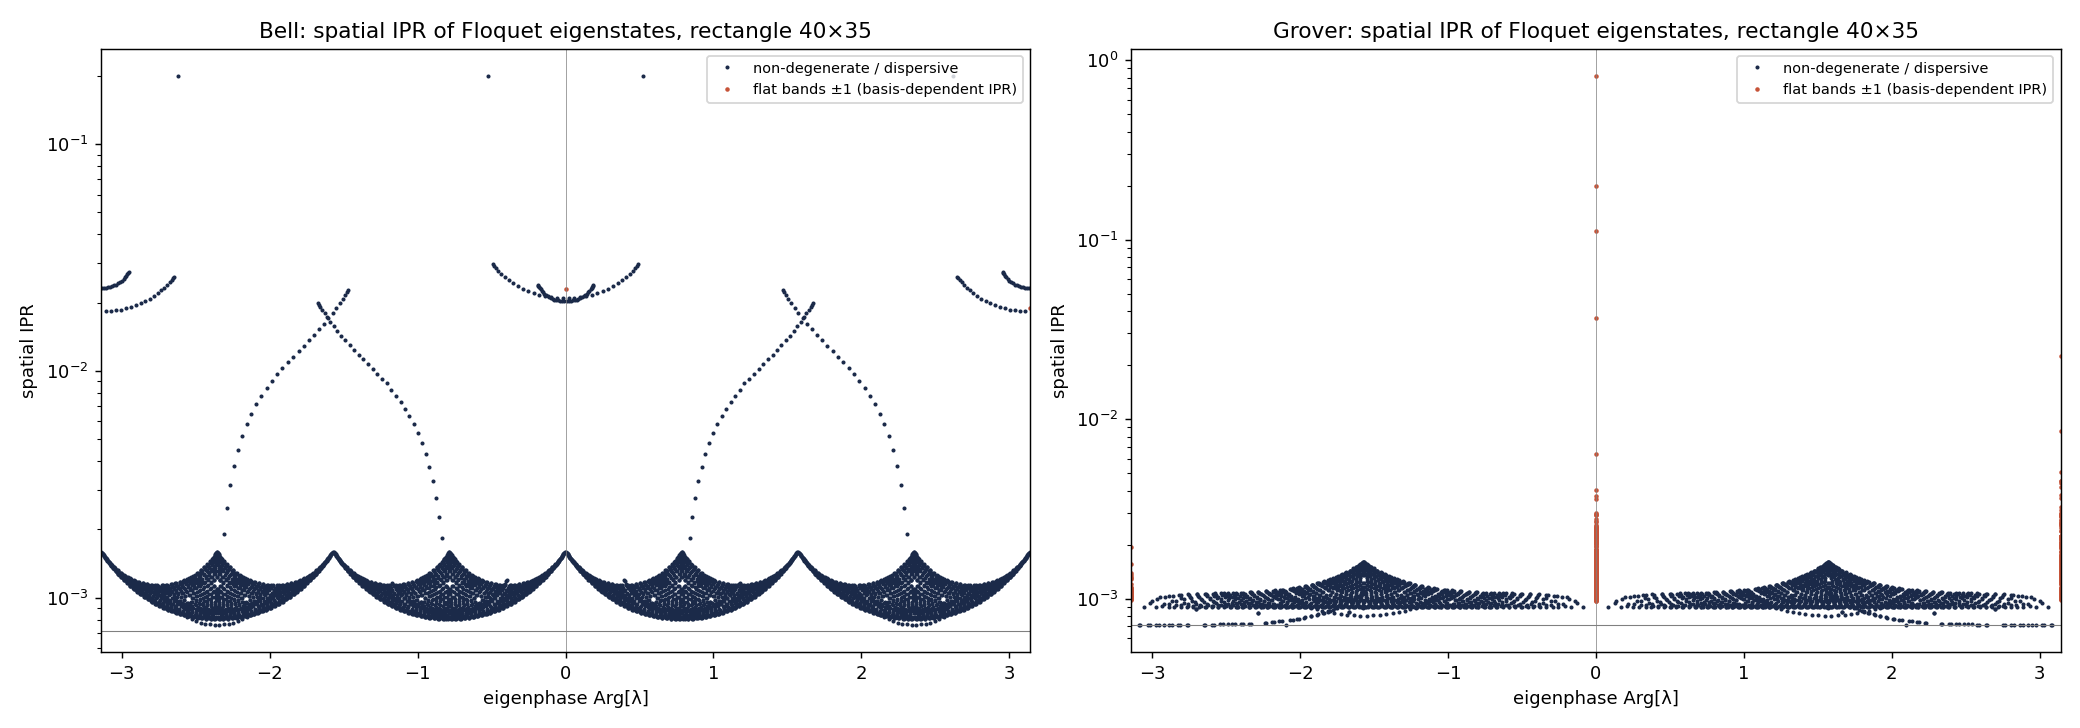
\includegraphics[width=\textwidth]{fig06_ipr_bellII_grover_40x35.png}
\caption{Spatial IPR of the Floquet eigenstates on a \(40\times35\)
rectangle. Left: Bell \(B_{\mathrm{II}}\). Right: Grover, where the
eigenvalues at exactly \(\pm1\) are drawn in red because their IPR is
basis-dependent. The grey line is \(1/V\). This reproduces the project's two IPR figures (the Bell one with
\(B_{\mathrm{II}}\), not \(B_{\mathrm I}\)).}
\label{fig:iprbase}
\end{figure}

\begin{figure}[htbp]
\centering
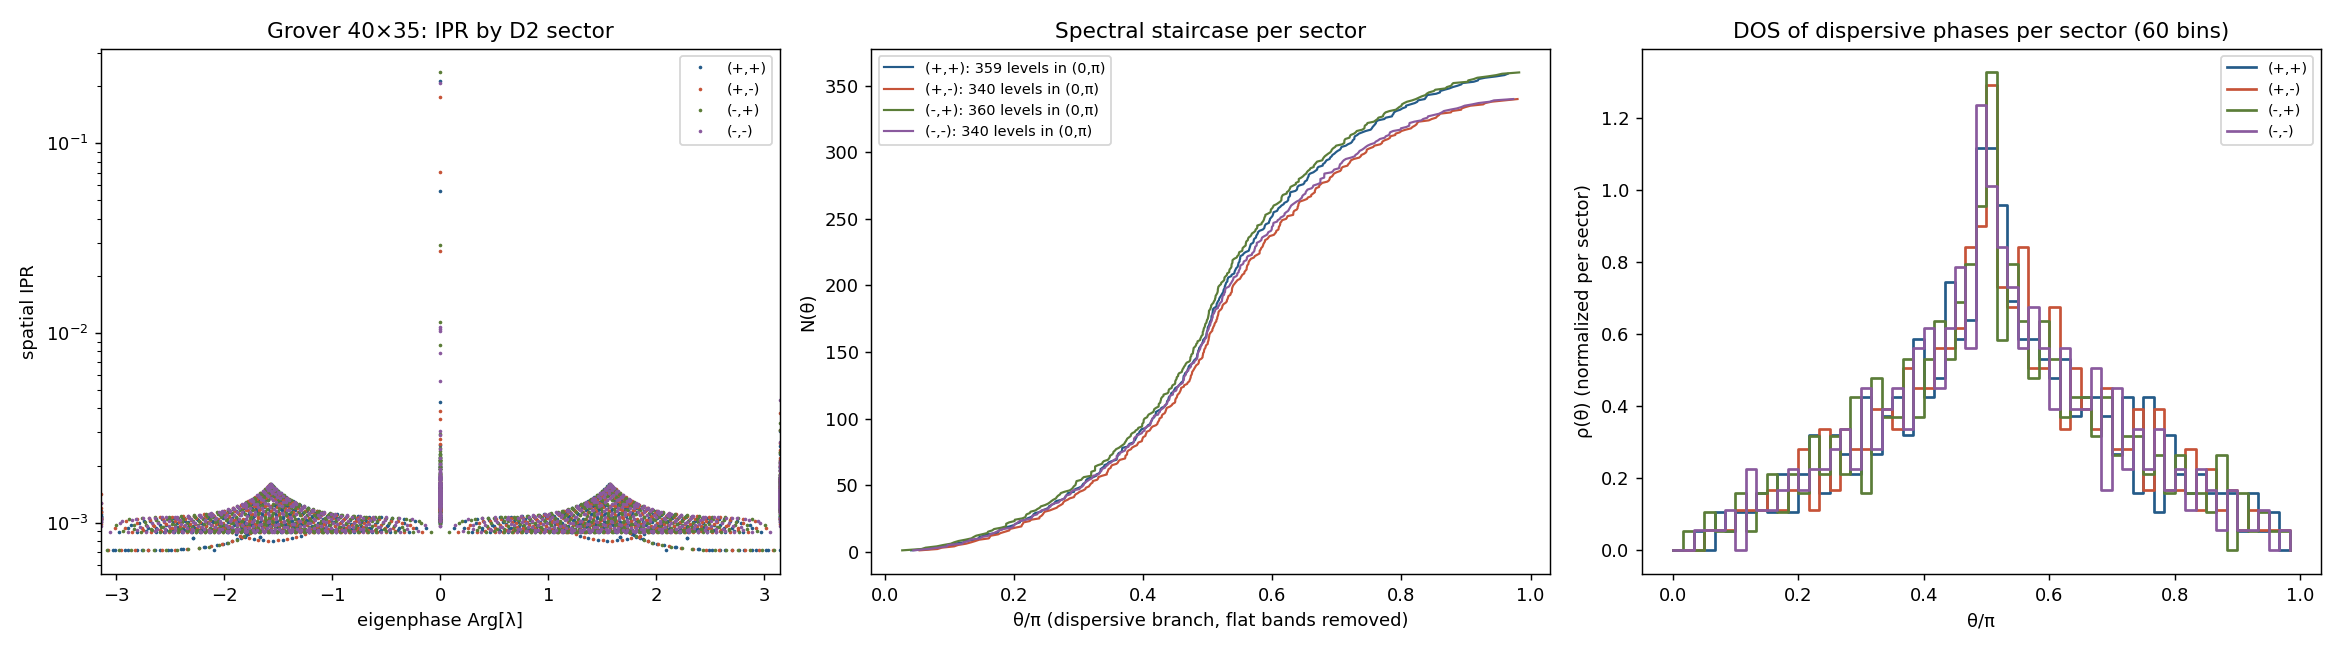
\includegraphics[width=\textwidth]{fig07_grover_sectors_40x35.png}
\caption{Grover on \(40\times35\), resolved into the four
\((p_x,p_y)\) sectors: IPR, spectral staircase of the dispersive branch,
and its density of states. The density peaks at \(\varphi=\pi/2\), the
van Hove point of the square lattice.}
\label{fig:groversectors}
\end{figure}

\section{Compass Fourier: an exact solution hidden by a gauge}
\label{sec:fourierfull}

Write \(U_{F}=S[\Id_{\mathrm{pos}}\otimes F_c]\). The gauge identity of
Appendix~\ref{app:gauge} with parameters \(\alpha=\pi\), \(\beta=0\)
reads
\begin{equation}
\boxed{W\ket{x,y,d}=(-1)^x\,\diag(-i,i,1,1)_{dd}\ket{x,y,d},\qquad
WU_FW^\dagger=S\,[\Id_{\mathrm{pos}}\otimes DF_cD],}
\end{equation}
with \(D=\diag(i,-i,1,1)\) as in Eq.~\eqref{eq:fouriergauge}. The
transformed coin is in the solvable family with \(C_+=i\sigma_x\),
\(e^{i\alpha}=-1\), \(e^{i\beta}=i\). The walk is therefore exactly solved
by the gauge-transformed standing-wave projectors \(W^\dagger P_aW\),
with blocks given by Eq.~\eqref{eq:generalblock}:
\begin{itemize}
\item the horizontal terminal states carry eigenvalue \(+1\) (\(N_y\) of
them);
\item the vertical terminal states carry eigenvalue \(-i\) (\(N_x\) of
them);
\item the \((0,0)\) block has eigenvalues \(\pm i\).
\end{itemize}
\session The operator identity holds to \(5\times10^{-32}\), and the
union of block spectra matches direct diagonalization of \(U_F\) to
\(5.7\times10^{-15}\) (\(7\times5\)) and \(1.3\times10^{-14}\)
(\(8\times6\)).

This replaces the earlier record that the Fourier endpoint was only
\emph{numerically} identified with the gauge orbit, without an explicit
transformation. A second check, also computed for this revision, on \(7\times5\) shows that
\(U_F\) commutes with \(\mathcal P_y\) and with the modified rotation
\(\mathcal R\widehat\Gamma\), \(\widehat\Gamma=\Id\otimes\diag(1,1,-1,-1)\),
but not with \(\mathcal R\) or \(\mathcal P_x\). The spectral statistics
of this exactly solved walk were not computed in this revision.

The physical-order coin \(F_p\) commutes with none of
\(\mathcal R,\mathcal R\widehat\Gamma,\mathcal P_x,\mathcal P_y\) on
\(7\times5\). Its full-walk status is open (Section~\ref{sec:fouriercoin}).

\section{Bell \(B_{\mathrm I}\): some symmetries survive, but a full solution is not established}
\label{sec:bellIfull}

Here \(B=B_{\mathrm I}\) and \(U_B=S[\Id_{\mathrm{pos}}\otimes B_{\mathrm I}]\).

For the explicit Bell matrix, \([B,J]=0\), so \(\mathcal R\)
commutes with \(U_B\). The walk is real, hence conjugate-paired,
and it has time reversal as described above. The separate rectangular
mirror symmetries do not follow from this coin.

The coin preserves the \(q_3\) pair label, but a boundary reversal
exchanges those pairs. Thus \([B,q_3]=0\) is not a conserved full-walk
label. The established mean leakage of that two-sector label is
\begin{equation}
\mathcal L_{q_3}(U_B)=\frac{N_x+N_y}{2N_xN_y}.
\end{equation}
There are \(2N_x+2N_y\) blocked directed channels among \(4N\)
basis states. An appropriate wall input can cross the pair partition
with probability one, so the worst-case leakage is one even when
the mean is small.

The Bell action on an antisymmetric horizontal mode contains
\begin{equation}
B\ket{g_m^x f_n^y;h_-}
=-\frac1{\sqrt2}\left(
\ket{g_m^x f_n^y;h_-}+\ket{g_m^x f_n^y;v_-}\right).
\end{equation}
The second term has the wrong envelope for the vertical antisymmetric
vector in \(\mathcal K_{mn}\), which requires \(f_m^xg_n^y\).
For the same nonterminal index,
\(\langle f_m^x,g_m^x\rangle=0\). Half the antisymmetric weight
leaks while the symmetric states remain within their sectors, giving
\begin{equation}
\boxed{\mathcal L_{\sw}(U_B)=\frac14.}
\end{equation}
Allowing deterministic relabeling of those mode sectors does not
reduce this value. Basis-state routing leakage is \(1/2\).

\recorded On \(25\times19\), the two rotation sectors give the
half-circle mean \(0.4872\) each, with 22 eigenvalues at each of
\(\pm1\) in each sector. On \(29\times22\), the corresponding
means are \(0.4940\) and \(0.4697\).

\open These results neither construct an integrable Bell reduction
nor demonstrate full random-matrix universality. Earlier broad claims
that the displayed Bell coin was already proved integrable are not
retained. Its complete structure remains an open part of the project.

\section{Bell \(B_{\mathrm{II}}\): a regular spectrum outside the tested families}
\label{sec:bellIIfull}

Write \(U_{B_{\mathrm{II}}}=S[\Id_{\mathrm{pos}}\otimes B_{\mathrm{II}}]\).

\textbf{Symmetries.} \([B_{\mathrm{II}},\sigma_x]\), \([B_{\mathrm{II}},\sigma_y]\)
and \([B_{\mathrm{II}},J]\) are all nonzero, so by Eq.~\eqref{eq:inherit}
none of \(\mathcal P_x,\mathcal P_y,\mathcal R\) survives.
\session Searches were run on \(7\times5\) and \(8\times6\), with
\(7\times6\) and \(8\times5\) for the unitary case. They covered
operators of the form (a rectangle site map in \(D_2\)) \(\times\) (a
constant or sublattice-dependent \(4\times4\) coin matrix). Within this
family they found:
\begin{itemize}
\item no commuting unitary other than the identity;
\item no reversing operator \(PUP^{-1}=U^{\mathsf T}\);
\item no spectral rotation \(VUV^\dagger=cU\) with \(c\in\{-1,\pm i\}\).
\end{itemize}
These restricted searches are not absence theorems. Since
\(B_{\mathrm{II}}\) is not symmetric, the time-reversal construction of
Section~\ref{sec:TR} does not apply either. The walk is real, so
\(KUK=U\) pairs \(e^{i\varphi}\) with \(e^{-i\varphi}\), and only
\((0,\pi)\) is used.

\textbf{Spectrum.} \session On \(40\times35\) (Figs.~\ref{fig:iprbase}
left and \ref{fig:bellIIspec}):
\begin{itemize}
\item one eigenvalue at each of \(\pm1\), 2799 in \((0,\pi)\), and exact
conjugate pairing;
\item \(\langle r\rangle=0.392\) on the half circle, with 14 zero gaps;
\item 5304 of the 5600 eigenvalues belong to exact \(\pi/2\) quartets:
\(e^{i\varphi}\), \(ie^{i\varphi}\), \(-e^{i\varphi}\) and
\(-ie^{i\varphi}\) all appear to \(10^{-9}\). This is why the bulk IPR
pattern repeats with period \(\pi/2\) and the density of states peaks at
\(\pm\pi/4,\pm3\pi/4\). No operator was found that implements the
quartets.
\end{itemize}
The 296 levels outside the quartets form the arcs near \(0\) and \(\pm\pi\)
and the branches rising toward \(\pm\pi/2\). They also include four
corner states.

\textbf{Corner states.} \session Four states sit at
\(\varphi=\pm\pi/6,\pm5\pi/6\), exact to \(10^{-12}\). They are
exponentially localized at the corners \((N_x,1)\) and \((1,N_y)\) and
have IPR \(0.200\) on every size tested: \(16\times13\), \(16\times14\),
\(17\times13\), \(17\times14\), \(20\times17\) and \(40\times35\). On
commensurate rectangles such as \(18\times12\), \(24\times12\) and
\(16\times16\), a bulk level coincides exactly with a corner state. The
eigensolver then returns an arbitrary mixture, and the plotted IPR becomes
basis-dependent. This explains the values near \(0.18\) and \(0.012\) at
these phases in the project's original Bell figure.

\textbf{Placement among the reduction families.} The forbidden weight is
\(5/8\) and the numerical gauge minimum \(1/2\). The coin is not monomial
(\(\mathcal M_{\mathrm{split}}=1/2\)), and it fully mixes the axis label
(\(\mathcal M_{q_1}=1\)), so it is not of row/column type. \open The
nearly Poisson half-circle statistic and the organized IPR families point
to an exact structure. It is not supplied by any of the four demonstrated
reduction families, and its origin, including the \(\pi/2\) quartets, is
an open question.

\begin{figure}[htbp]
\centering
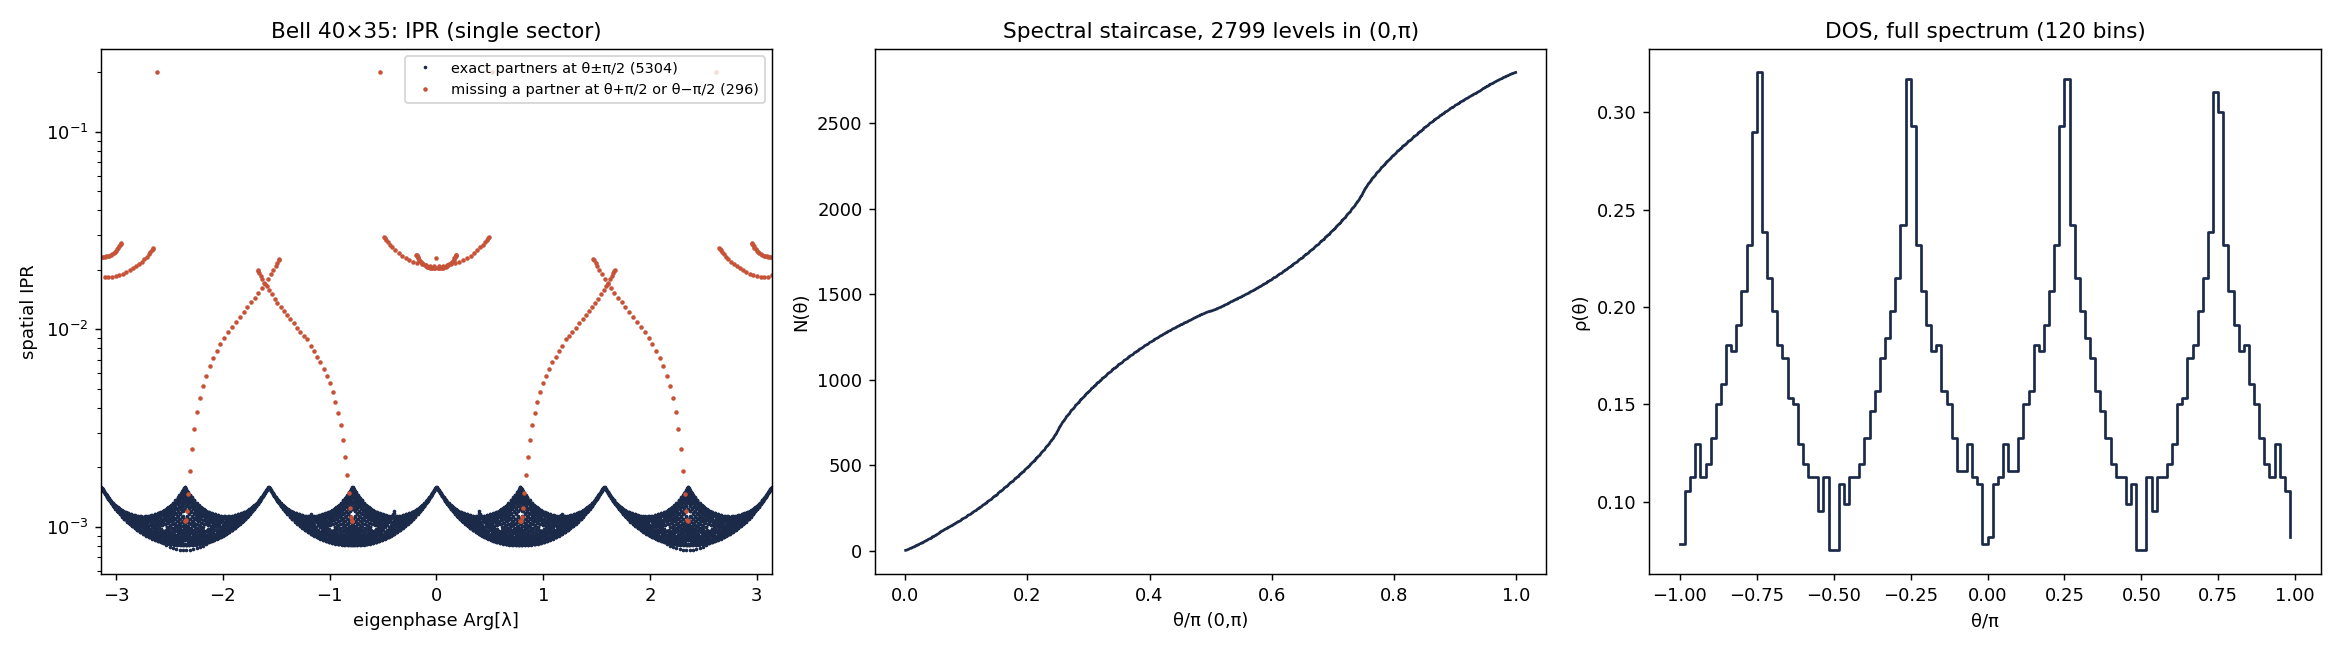
\includegraphics[width=\textwidth]{fig08_bellII_spectrum_40x35.png}
\caption{Bell \(B_{\mathrm{II}}\) on \(40\times35\). Left: IPR, with
levels outside the exact \(\pi/2\) quartets in red. Centre: spectral
staircase on \((0,\pi)\). Right: density of states of the full circle.}
\label{fig:bellIIspec}
\end{figure}

\section{Modified Grover: how the coin couples mode labels}
Write \(U_G(\theta)=S[\Id_{\mathrm{pos}}\otimes C_G(\theta)]\); thus \(U_G(0)=U_G\).

The odd components that \(C_G(\theta)\) couples require different
envelopes: \(g_m^xf_n^y\) for \(h_-\) and \(f_m^xg_n^y\) for
\(v_-\). The onsite coin changes the coin vector without changing
the spatial profile. Its output must therefore be re-expanded in
other mode labels. The cross-mode coefficients contain
\begin{equation}
\langle f_p^x,g_m^x\rangle\langle g_q^y,f_n^y\rangle.
\end{equation}
Reflection parity makes a nonzero term require both \(p+m\) and
\(q+n\) odd. Many fine labels can couple while their combined
rotation parity remains fixed.

The established exact diagnostics are
\begin{equation}
\boxed{
\mathcal L_{\sw}(U_G(\theta))=\tfrac12\sin^2\theta,\qquad
\mathcal M_{\mathrm{dir}}(C_G(\theta))=\cos^2\theta.
}
\end{equation}
Thus decreasing the minimum direction-pair score can increase this
spatial-mode leakage. These numbers measure different structures.
At \(\theta=\pi/3\) they are \(3/8\) and \(1/4\), respectively.
At \(\theta=0\) and \(\pi\), the fixed standing-wave blocks are
preserved again.

\subsection{The surviving symmetries}

The rotation \(\mathcal R\) survives throughout. The verified
time reversal
\(A=\CC_G(\theta)^\dagger\mathcal J K\) squares to one and
preserves its sectors. The commuting antiunitaries
\(\mathcal P_xK\) and \(\mathcal P_yK\) also preserve each rotation
sector, pairing \(\varphi\) with \(-\varphi\). Here
\(\CC_G(\theta)=\Id_{\mathrm{pos}}\otimes C_G(\theta)\).

Define \(\Gamma=\diag(1,1,-1,-1)\) and
\(\widehat{\Gamma}=\Id_{\mathrm{pos}}\otimes\Gamma\).
Another exact identity is
\begin{equation}
U_G(\pi-\theta)=-\widehat{\Gamma} U_G(\theta)\widehat{\Gamma}.
\end{equation}
At \(\theta=\pi/2\), \(\widehat{\Gamma} U\widehat{\Gamma}=-U\),
and the additional recorded quarter-circle relation is
\begin{align}
W_0\ket{x,y,d}&=(-1)^{x+y}
\diag(-i,i,-i,i)_{dd}\ket{x,y,d},\\
V_0&=W_0\mathcal P_x,\qquad V_0UV_0^\dagger=iU,\\
V_0\mathcal R&=(-1)^{N_x+N_y+1}\mathcal R V_0.
\end{align}
An operator rotating the spectrum by a phase is not a commuting
symmetry. These extra relations make this parameter special.

\subsection{Recorded spectral evidence}

For generic parameters the audit selects
\(10^{-7}<\varphi<\pi-10^{-7}\) in each rotation sector. It uses
noncyclic gaps, sets gaps below \(10^{-9}\) to zero, keeps isolated
zero-gap ratios, and omits undefined \(0/0\) ratios with a count.
At \(\theta=\pi/3\), the recorded and independently reproduced
values are
\begin{center}
\begin{tabular}{@{}lrrrr@{}}
\toprule
Rectangle&\(\langle r\rangle_+\)&Ratios&\(\langle r\rangle_-\)&Ratios\\
\midrule
\(17\times13\)&0.534116&218&0.539212&219\\
\(23\times17\)&0.523110&388&0.526623&389\\
\(31\times23\)&0.536581&710&0.532719&711\\
\(41\times29\)&0.522816&1186&0.519234&1187\\
\bottomrule
\end{tabular}
\end{center}
The source reports aspect-ratio and distribution checks as well;
Appendix~\ref{app:record} preserves their scope. These results support
orthogonal-class local repulsion at a deterministic coin. They do not
establish an exhaustive absence of other conserved structures.

\begin{figure}[htbp]
\centering
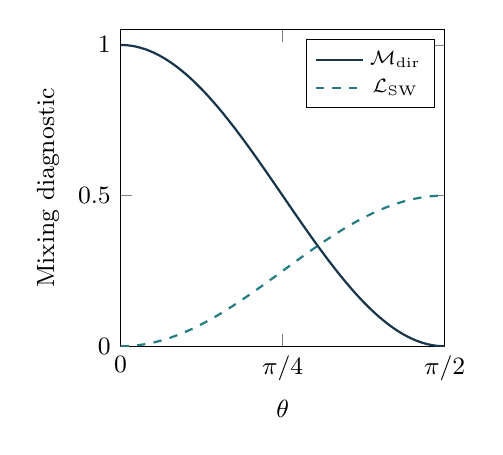
\begin{tikzpicture}
\begin{axis}[width=.47\textwidth,height=5.6cm,
xlabel={\(\theta\)},ylabel={Mixing diagnostic},xmin=0,xmax=1.5708,
ymin=0,ymax=1.05,xtick={0,.785398,1.570796},
xticklabels={\(0\),\(\pi/4\),\(\pi/2\)},
legend style={font=\scriptsize,at={(.97,.97)},anchor=north east},
tick label style={font=\small},label style={font=\small}]
\addplot[ink,thick,domain=0:1.570796,samples=90]{cos(deg(x))^2};
\addlegendentry{\(\mathcal M_{\mathrm{dir}}\)}
\addplot[accent,thick,dashed,domain=0:1.570796,samples=90]{.5*sin(deg(x))^2};
\addlegendentry{\(\mathcal L_{\sw}\)}
\end{axis}
\end{tikzpicture}\hfill
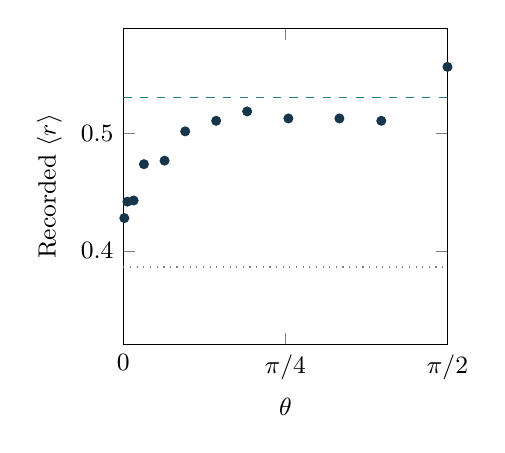
\begin{tikzpicture}
\begin{axis}[width=.47\textwidth,height=5.6cm,
xlabel={\(\theta\)},ylabel={Recorded \(\langle r\rangle\)},
xmin=0,xmax=1.5708,ymin=.32,ymax=.59,
xtick={0,.785398,1.570796},xticklabels={\(0\),\(\pi/4\),\(\pi/2\)},
tick label style={font=\small},label style={font=\small}]
\addplot[ink,only marks,mark=*,mark size=1.6pt] coordinates {
(.005,.428)(.02,.442)(.05,.443)(.1,.474)(.2,.477)
(.3,.502)(.45,.511)(.6,.519)(.8,.513)(1.047198,.513)
(1.25,.511)(1.570796,.557)};
\addplot[accent,dashed,domain=0:1.570796]{.5307};
\addplot[gray,dotted,domain=0:1.570796]{.386294};
\end{axis}
\end{tikzpicture}
\caption{Left: the already established exact diagnostics for the
modified Grover family. Right: recorded half-circle, rotation-resolved
pooled means on \(25\times19\), redrawn from the supplied export;
no spectra were recomputed. Dashed and dotted references are the
orthogonal and Poisson values. The degenerate Grover endpoint is not
plotted. The point \(\pi/2\) has additional exact symmetries and
cannot be read as a generic crossover endpoint.}
\end{figure}

\subsection{What zero direction-pair mixing means at the special point}

At \(\theta=\pi/2\),
\begin{equation}
C_G(\pi/2)=\frac12\begin{pmatrix}
0&0&1+i&1-i\\0&0&1-i&1+i\\
1+i&1-i&0&0\\1-i&1+i&0&0
\end{pmatrix}.
\end{equation}
It always swaps the axes, so \(\mathcal M_{q_1}=0\), while a
definite input direction still splits into two outputs. Its splitting
entropy is \(1/2\), and \(\mathcal L_{\sw}=1/2\).

Recorded half-circle means are about \(0.55\) on tested odd-by-odd
rectangles, but only \(0.4361,0.4487\) in the two sectors on
\(29\times18\). The latter half-circle contains degenerate phases
at \(i\); its quoted filtering discards undefined pairs. The supplied teaching source additionally records quarter-window checks giving
\(0.5554,0.5495,0.5565\) on \(17\times13,23\times17,25\times19\),
respectively, and approximately \(0.4386,0.4504\) in the two sectors
on \(29\times18\). Symmetry-related copies are not independent
samples. The parity effect remains unexplained; the point is not an
established all-size chaos example.


\subsection{Results computed for this revision: the full interval on \(31\times23\)}

\session The rotation sectors are resolved with the full operator
\(\mathcal R\) (site rotation \(\times\) \(J\)). Within each sector only
the half circle \(0<\varphi<\pi\) is used, because \(\mathcal P_xK\)
pairs \(\varphi\) with \(-\varphi\); flat \(\pm1\) phases are removed.
At \(\theta=0\) the four parity sectors are resolved instead. We also re-verified that
\begin{itemize}
\item \(\mathcal R\) is the only commuting operator among (site map)
\(\times\) (constant coin matrix);
\item a time reversal with square \(+1\) exists, and \(\mathcal P_xK\),
\(\mathcal P_yK\) commute with the walk;
\item \(U_G(\pi-\theta)=-\widehat\Gamma U_G(\theta)\widehat\Gamma\) holds
to \(4\times10^{-15}\).
\end{itemize}
The finite-size orthogonal reference was obtained from GOE matrices of
the same two sector sizes, processed identically: \(0.530\pm0.010\)
(20 replicas).
\begin{center}\small
\begin{tabular}{@{}lccccccccccc@{}}\toprule
\(\theta/\pi\)&0&0.05&0.10&0.15&0.20&0.25&0.30&0.35&0.40&0.45&0.50\\\midrule
\(\langle r\rangle\)&0.411&0.476&0.488&0.500&0.512&0.521&0.521&0.535&0.537&0.509&0.548\\\bottomrule
\end{tabular}
\end{center}
Statistical errors are about \(\pm0.007\); at \(\theta=0\) the error is
\(\pm0.011\) with 704 ratios, and for \(\theta>0\) there are 1421 ratios.
Additional angles give \(0.486\) (\(\pi/32\)), \(0.502\) (\(\pi/16\)) and
\(0.535\) (\(\pi/3\)). The last agrees with the recorded rotation-sector
values \(0.5366\) and \(0.5327\) on the same rectangle in the table above,
which is an independent reproduction.

Size checks at \(\theta=\pi/4\) give \(0.498\pm0.011\) (\(21\times15\))
and \(0.515\pm0.005\) (\(41\times31\)). At \(3\pi/8\) they give
\(0.512\pm0.010\) and \(0.516\pm0.005\). The \(41\times31\) values lie
slightly below the orthogonal reference. The point \(0.45\pi\) is about
\(2\sigma\) below its neighbours and was not rechecked.

The IPR collage, Fig.~\ref{fig:collagegrover}, shows the same crossover
in the eigenstates. At \(\theta=0\) there are smooth families and red
flat bands. By \(\theta=\pi/32\) the flat bands are gone and the families
begin to break. From about \(\pi/4\) the bulk IPR collapses into a
narrow, featureless band, as expected for eigenstates spread over the
whole rectangle.

\begin{figure}[htbp]
\centering
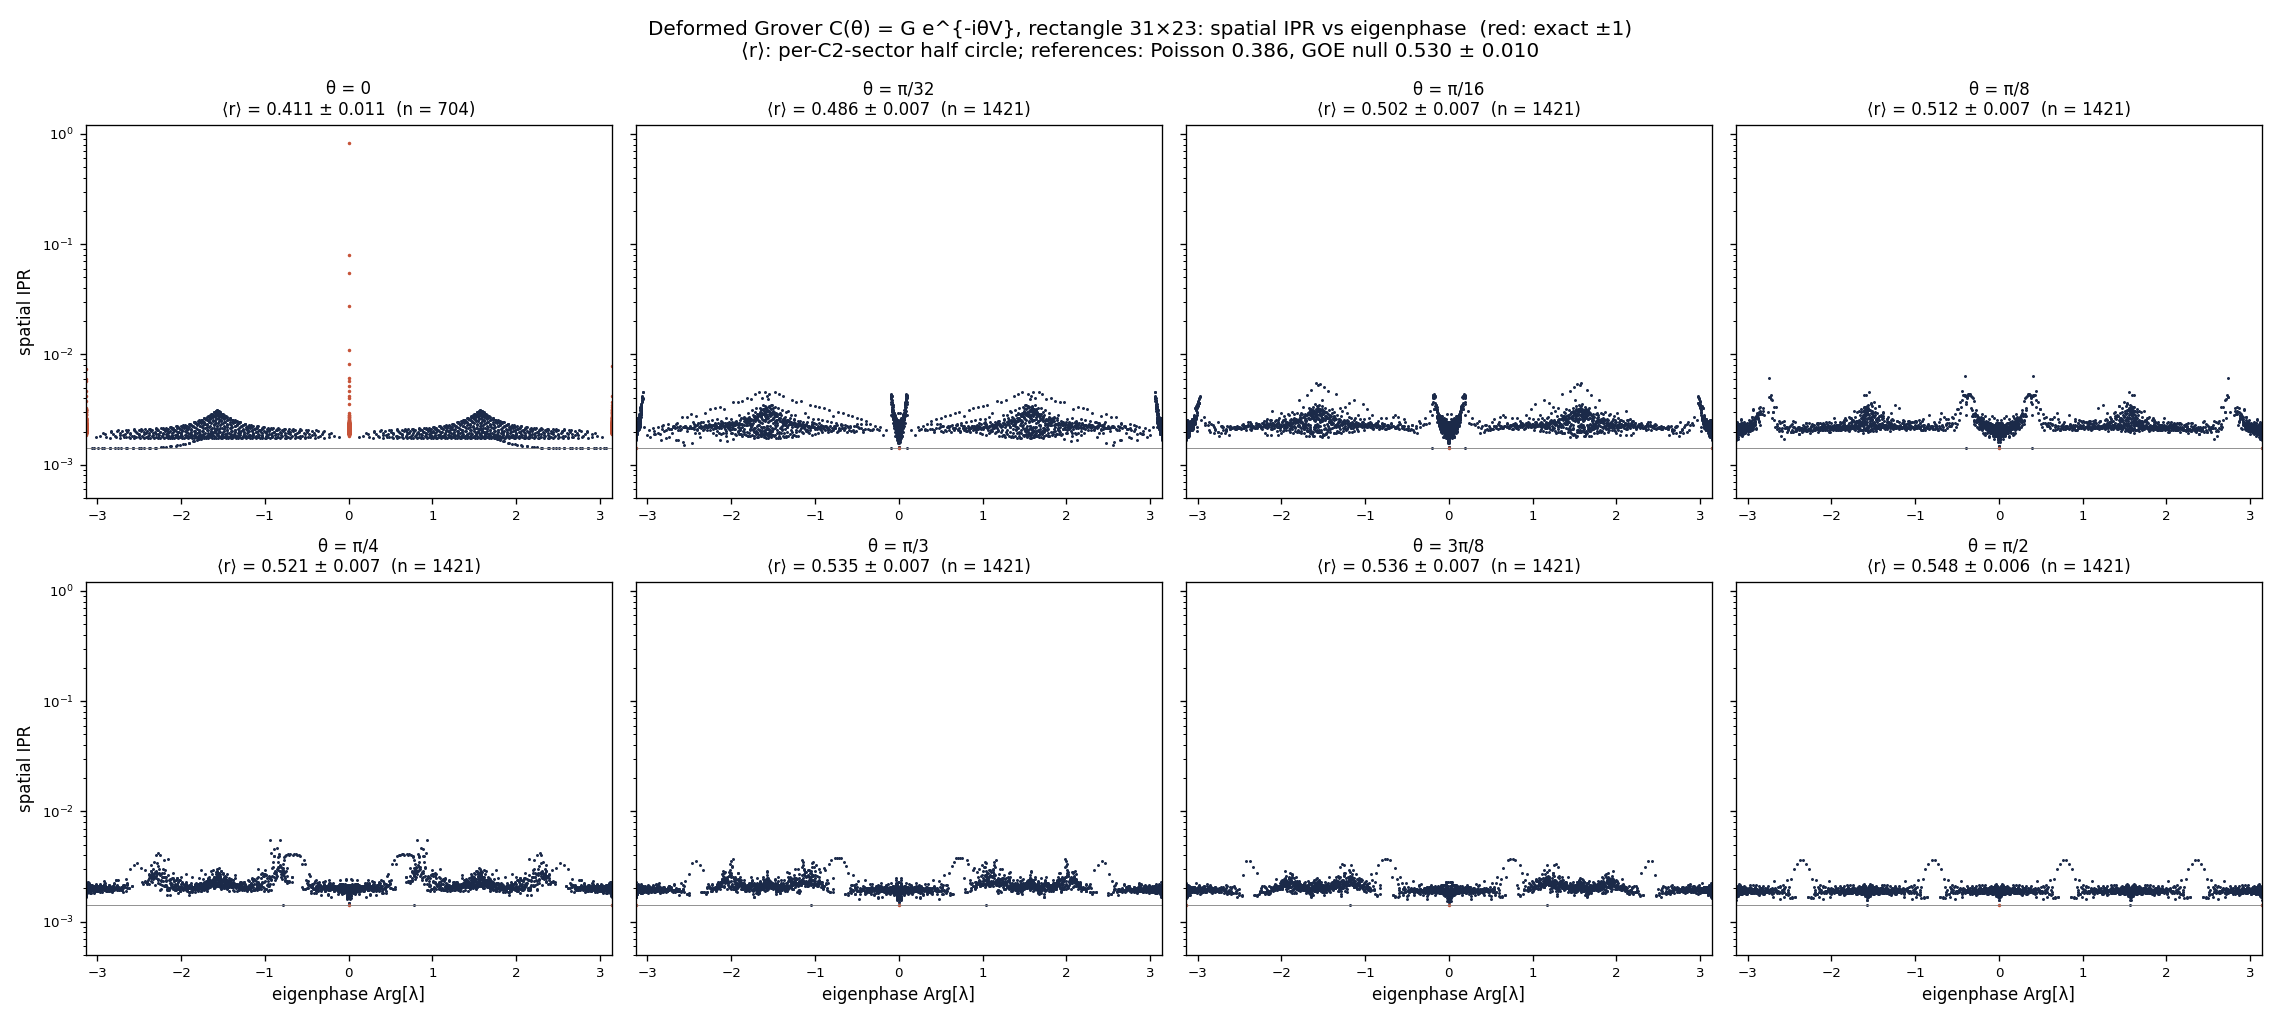
\includegraphics[width=\textwidth]{fig09_ipr_collage_modified_grover.png}
\caption{Spatial IPR of the modified Grover walk \(U_G(\theta)\) on
\(31\times23\) for eight values of \(\theta\). Each panel title gives the
sector-resolved half-circle \(\langle r\rangle\). Red points are exact
\(\pm1\) eigenvalues, with basis-dependent IPR.}
\label{fig:collagegrover}
\end{figure}

\section{Modified Bell: the exact structures break, chaos is not reached}
\label{sec:modbellfull}

Write \(U_B(\theta)=S[\Id_{\mathrm{pos}}\otimes B_{\mathrm{II}}(\theta)]\).

\textbf{Symmetries.} \session For \(\theta\ne0,\pi\), the search
described for \(B_{\mathrm{II}}\) was extended to commuting antiunitaries
\(RU^{*}=UR\) and to reversing antiunitaries \(RU^{*}=U^\dagger R\), with
the same restricted family of \(R\) on \(7\times5\). It found nothing
besides the identity. The coin is complex and not symmetric, so neither
the reality pairing nor the Section~\ref{sec:TR} time reversal is
available. A single sector and the \emph{full} circle are used, with
cyclic gaps. If no antiunitary exists, the relevant reference would be
the unitary class, \(\langle r\rangle\approx0.600\). The finite-size CUE
value for 2852 levels was \(0.599\). At \(\theta=0,\pi\) the walk is real
and the half circle is used.

\textbf{Exact structures disappear.} \session On \(31\times23\), the
fraction of eigenvalues in exact \(\pi/2\) quartets is \(0.926\) at
\(\theta=0\) and at \(\theta=\pi\). It is exactly \(0\) at the nine
interior grid points \(\theta=0.1\pi,\ldots,0.9\pi\). The conjugate
pairing behaves the same way: \(100\%\) at the endpoints and \(0\%\) in
between.

\textbf{Level statistics.} \session On \(31\times23\) (half circle at the
endpoints with 1424 ratios, full circle otherwise with 2852 ratios,
errors about \(\pm0.005\)):
\begin{center}\small
\begin{tabular}{@{}lccccccccccc@{}}\toprule
\(\theta/\pi\)&0&0.1&0.2&0.3&0.4&0.5&0.6&0.7&0.8&0.9&1\\\midrule
\(\langle r\rangle\)&0.402&0.431&0.453&0.470&0.495&0.457&0.495&0.484&0.467&0.445&0.399\\\bottomrule
\end{tabular}
\end{center}
Additional angles give \(0.409\) (\(\pi/16\)), \(0.440\) (\(\pi/8\)),
\(0.483\) (\(\pi/4\)), \(0.502\) (\(5\pi/8\)) and \(0.496\)
(\(3\pi/4\)). At \(\theta=0.4\pi\) the size dependence is \(0.500\pm0.007\)
(\(21\times15\)), \(0.495\pm0.005\) (\(31\times23\)) and \(0.488\pm0.004\)
(\(41\times31\)), drifting slightly downward. At \(\pi/2\) it is
\(0.479\pm0.008\) (\(21\times15\)) and \(0.457\pm0.005\) (\(31\times23\)).
The statistic stays well below both the unitary and the orthogonal
references over the whole interval.

\textbf{Eigenstates.} In the IPR collage, Fig.~\ref{fig:collagebell}, the
bulk keeps its regular scalloped pattern at every angle. Only the states
near the walls, the arcs and isolated points with IPR between about
\(0.01\) and \(0.5\), are scrambled. At \(\theta=\pi\) the full regular
pattern returns.

\textbf{An explanation that was tested and rejected.} One might think the
rotation leaves the bulk band structure unchanged and acts only through
the walls. \session This is false. On the infinite lattice, for 200
random wavevectors, the bulk eigenphases of
\(\Lambda(k_x,k_y)B_{\mathrm{II}}(\theta)\) differ from those at
\(\theta=0\) by up to \(0.21\), \(0.61\), \(0.97\) and \(1.24\) rad at
\(\theta=0.3,0.9,1.5,2.5\). Why the bulk eigenstates stay organized
remains unexplained.

\begin{figure}[htbp]
\centering
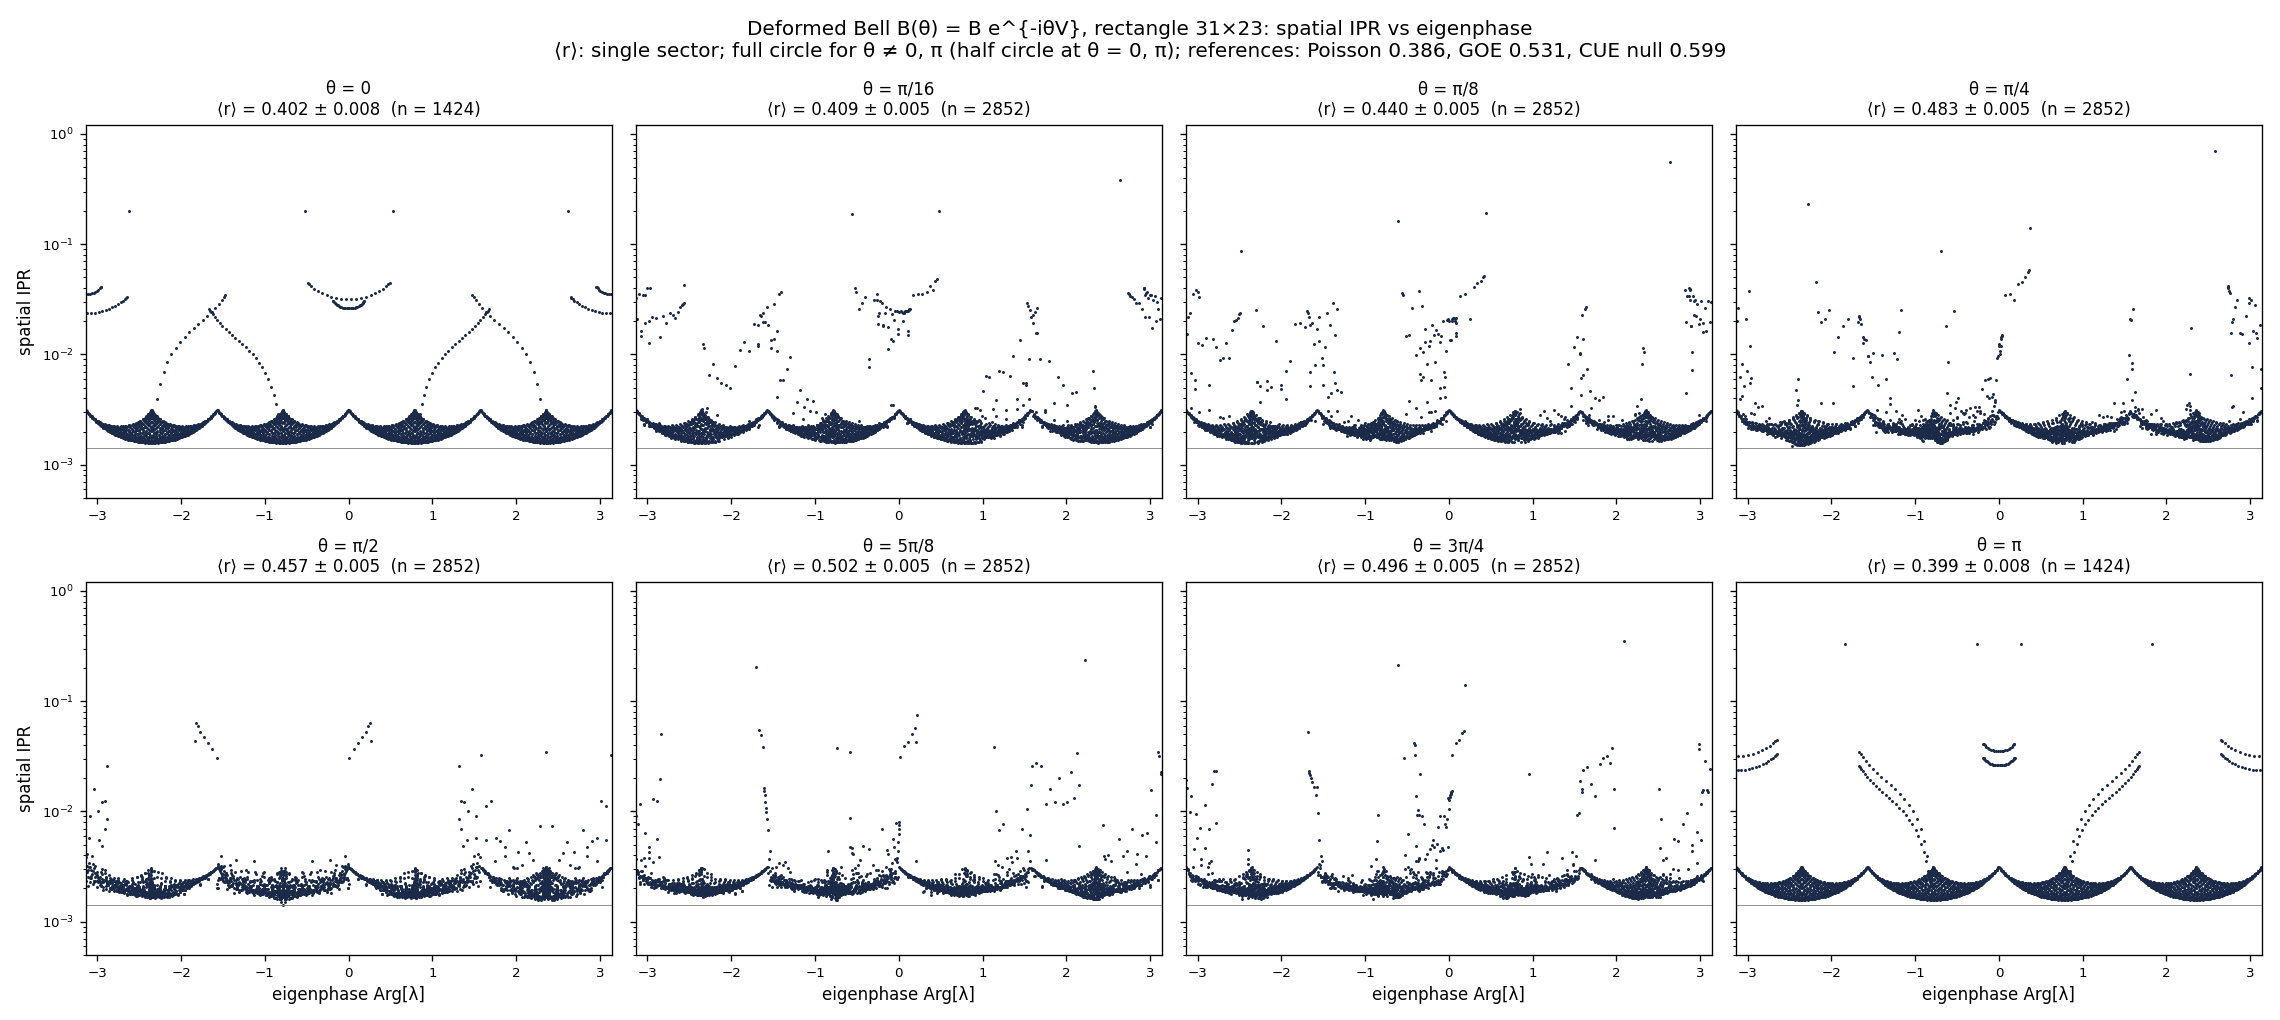
\includegraphics[width=\textwidth]{fig10_ipr_collage_modified_bellII.png}
\caption{Spatial IPR of the modified Bell walk \(U_B(\theta)\) on
\(31\times23\) for eight values of \(\theta\in[0,\pi]\). Each panel
title gives \(\langle r\rangle\): single sector, full circle for
\(\theta\neq0,\pi\).}
\label{fig:collagebell}
\end{figure}

\begin{figure}[htbp]
\centering
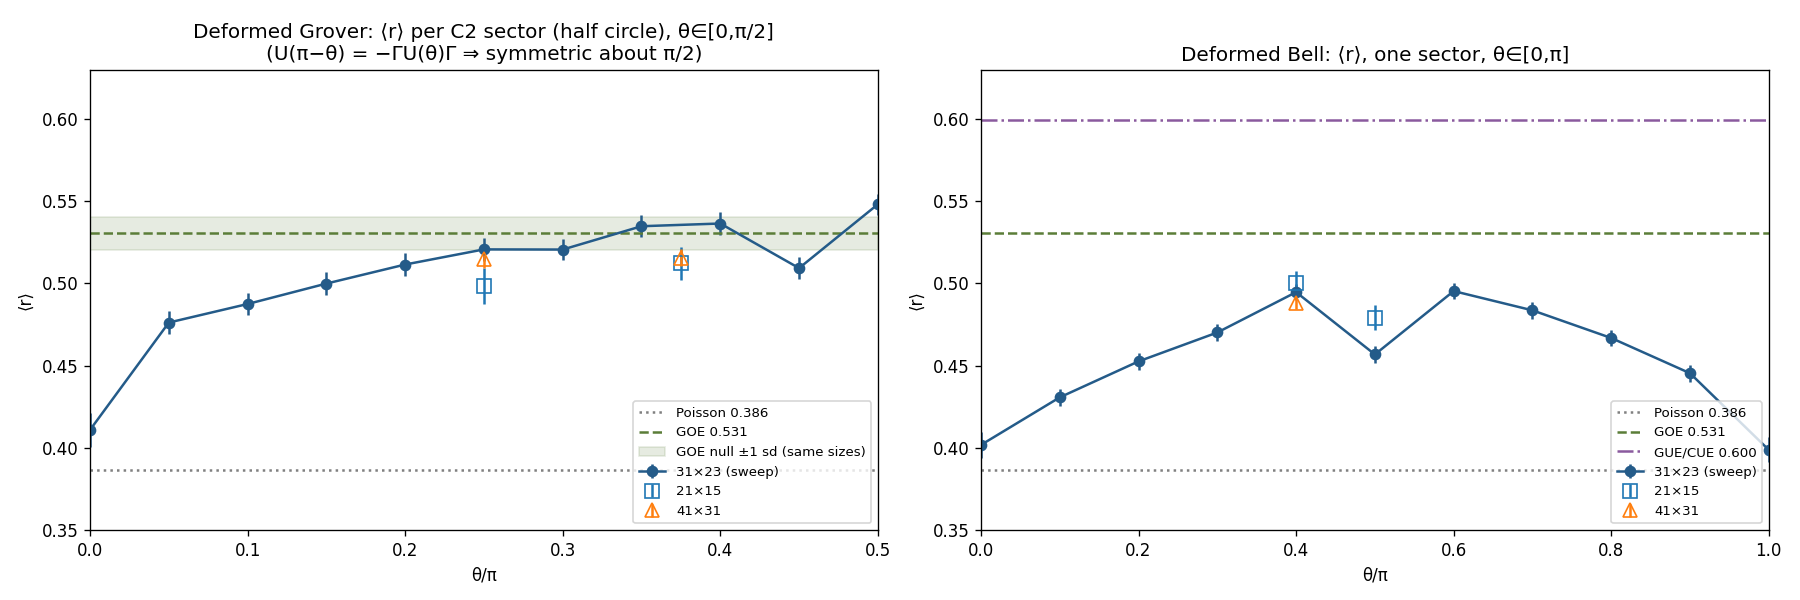
\includegraphics[width=\textwidth]{fig11_r_vs_theta.png}
\caption{\(\langle r\rangle\) versus \(\theta\) for the modified Grover
(left; rotation sectors, half circle; band = finite-size GOE null
\(\pm1\) s.d.) and modified Bell (right; single sector) walks on
\(31\times23\), with size checks on \(21\times15\) and \(41\times31\).}
\label{fig:rtheta}
\end{figure}

\section{What the examples have established}

\begin{center}
\small
\begin{tabularx}{\textwidth}{@{}lYY@{}}
\toprule
Coin&Established full-walk structure&Current conclusion\\
\midrule
Identity \(\Id\)&The shift's own row and column cycles (Section~\ref{sec:identitycoin})&Exact; maximally degenerate spectrum\\
Permutation \(P\)&Complete deterministic basis cycles&Exact cycle solution\\
Grover \(G\)&Complete standing-wave blocks, size at most four&Exact rectangular solution; Poisson-like resolved statistics, flat bands\\
Compass Fourier \(F_c\)&Gauge-transformed standing-wave blocks (explicit \(W\))&Exact rectangular solution; statistics not computed\\
Physical Fourier \(F_p\)&None found; outside tested families&Open; walk not examined\\
Bell \(B_{\mathrm I}\)&Rotation and antiunitary relations; \(\mathcal L_{\sw}=\mathcal L^*_{\sw}=\tfrac14\)&Intermediate recorded \(\langle r\rangle\); classification open\\
Bell \(B_{\mathrm{II}}\)&Reality pairing; exact \(\pi/2\) quartets for \(95\%\) of levels; corner states; no geometric symmetry found&Regular-looking (\(\langle r\rangle\approx0.39\)) but outside tested families; open\\
Modified Grover&Rotation and time reversal; envelope leakage \(\tfrac12\sin^2\theta\)&Orthogonal-class-like local statistics from \(\theta\approx\pi/4\) at tested sizes\\
Modified Bell&No symmetry found for \(\theta\neq0,\pi\); quartets and pairing destroyed; \(\mathcal L_{\sw}=5/8\) constant&Exact structures broken, statistics intermediate (\(\le0.50\)); no RMT class reached\\
\bottomrule
\end{tabularx}
\end{center}

\section{A checklist for teaching a selected coin}

\begin{enumerate}
\item Read the explicit matrix in the fixed direction order.
Its name is not a shift convention or a symmetry proof.
\item Return to the row/column, parity and standing-wave structures
supplied before choosing the coin.
\item Test the full-space commutators. Distinguish commuting symmetries
from reversers, conjugate pairing and spectral rotations.
\item Display a complete cycle or mode construction when one exists.
A few surviving parity sectors only organize the unresolved dynamics.
\item State spectral evidence with its sectors, windows, degeneracy
rule and finite-size scope. For both Bell walks, keep the classification open.
\item Draw the 16-cell coherent square with the envelope mask, and compute
its gauge minimum, before interpreting any leakage.
\end{enumerate}

\begin{lesson}{The full reasoning chain}
First identify the structures supplied by the shift and rectangle.
Next test how the coin acts on them. A complete explicit reduction
can establish exact solvability; a surviving coarse symmetry only
defines sectors. If no complete reduction is known, use correctly
resolved spectral evidence and state its scope. Neither local
direction splitting nor leakage from one selected mode family is,
by itself, a necessary-and-sufficient detector of quantum chaos.
\end{lesson}



\chapter{Routes out of exact solvability in the fixed rectangle}
\label{ch:mechanisms}

The rectangle and the stay-and-reverse shift are fixed; only the coin
changes. In this chapter, \emph{breaking integrability} is used in a
deliberately operational sense, with two parts. Structurally, the walk
leaves every demonstrated reduction family. Spectrally, correctly
resolved local statistics move from Poisson-like values toward a
random-matrix reference. Neither part is decisive on its own: a structure
outside the tested families may exist, and a spacing statistic is not a
proof. The goal here is to describe the routes observed so far, not to
decide whether they are one mechanism.

\section{The reduction families as label algebras supplied by the geometry}

Each demonstrated family is a set of projectors built from the rectangle
and the shift \emph{before} the coin is chosen, together with the coin
condition that keeps them conserved:
\begin{center}\small
\begin{tabularx}{\textwidth}{@{}lYYY@{}}\toprule
Family&Geometric projectors&Coin condition&Fingerprint in the 16-cell map\\\midrule
Rows/columns&\(P^H_y,\,P^V_x\)&\(C=C_H\oplus C_V\) in \(\{R,L\}\mid\{U,D\}\)&Physical square block diagonal by axis\\
Standing waves&\(P_a\in\mathscr P_{\sw}\)&\(\widetilde C=C_+\oplus e^{i\alpha}\oplus e^{i\beta}\)&No weight in the ten forbidden cells\\
Gauge images&\(W^\dagger P_aW\)&\(\mathcal L^*_{\sw}=0\)&Forbidden cells empty after \(C\to DCD\)\\
Routing&Position--direction basis&Monomial coin&One nonzero cell per physical column\\\bottomrule
\end{tabularx}
\end{center}
In the language of Appendix~\ref{app:advanced}, each family is a
commutative label algebra. Exact solvability within the family means
that conjugation by \(U\) maps the algebra into itself, so that its
escape \(\mathcal M^{\mathrm{alg}}\) vanishes.

\section{Where each coin sits}

\begin{center}\small
\begin{tabularx}{\textwidth}{@{}lccccccY@{}}\toprule
Coin&\(\mathcal L_{\sw}\)&\(\mathcal L^*_{\sw}\)&\(\mathcal M_{\mathrm{split}}\)&\(\mathcal M_{q_1}\)&\([C,J]=0\)&\(C=C^{\mathsf T}\)&Family / status\\\midrule
\(\Id\)&0&0&0&0&yes&yes&All four families; exact, maximally degenerate\\
\(P\)&\(1/2\)&\(\le1/2\)&0&0&yes&yes&Routing; exact\\
\(G\)&0&0&1&1&yes&yes&Standing waves; exact\\
\(F_c\)&\(1/2\)&0&1&1&no&yes&Gauge image; exact\\
\(F_p\)&\(9/16\)&\(\le0.073\)&1&1&no&yes&None found; open\\
\(B_{\mathrm I}\)&\(1/4\)&\(\le1/4\)&\(1/2\)&1&yes&yes&None found; open\\
\(B_{\mathrm{II}}\)&\(5/8\)&\(\le1/2\)&\(1/2\)&1&no&no&None found; regular-looking, open\\
\(C_G(\theta)\)&\(\tfrac12\sin^2\theta\)&\(\tfrac12\sin^2\theta\)&varies&\(\cos^2\theta\)&yes&yes&Leaves standing waves for \(0<\theta<\pi\)\\
\(B_{\mathrm{II}}(\theta)\)&\(5/8\)&\(0.444\)--\(0.5\)&varies&1&no&no&None found; exact structures broken\\\bottomrule
\end{tabularx}
\end{center}
Values marked \(\le\) are numerical gauge minima, which are upper bounds.
The entries for \(C_G(\theta)\) are exact; Appendix~\ref{app:gauge} gives
the proof of its gauge minimum. The splitting entropy of \(C_G\) is
\(0.906\) at \(\pi/4\) and \(0.772\) at \(\pi/3\); that of
\(B_{\mathrm{II}}(\pi/4)\) is \(0.80\).

\section{Route 1: envelope mismatch (modified Grover)}

The rotation \(e^{-i\theta V}\) acts on the antisymmetric inputs, which
for Grover start entirely in their allowed diagonal cells. It moves the
weight \(\sin^2\theta\) of each into the cell \(h_-\leftrightarrow v_-\).
That cell is forbidden because it exchanges the envelope \(g^xf^y\) with
\(f^xg^y\) (Section~\ref{sec:envelope}). Physically, a standing wave
whose sine runs along \(x\) is converted, at every site, into the channel
whose sine must run along \(y\). The output has to be re-expanded in other
mode labels, with overlaps
\(\langle f_p^x,g_m^x\rangle\langle g_q^y,f_n^y\rangle\) that couple many
\((p,q)\) to \((m,n)\) (\(p+m\) and \(q+n\) odd). On the recorded
\(9\times7\) example this coupling already merges the 79 standing-wave
sectors into three components (Appendix~\ref{app:advanced}).

Three findings show that this route is genuine and not a basis artifact:
\begin{enumerate}
\item the leakage cannot be removed by a gauge:
\(\mathcal L^*_{\sw}=\mathcal L_{\sw}=\tfrac12\sin^2\theta\), exactly;
\item \(\langle r\rangle\) rises together with the leakage, from 0.41 to
the orthogonal reference by \(\theta\approx\pi/4\)
(Fig.~\ref{fig:mechanisms}(a));
\item the eigenstates spread over the whole rectangle
(Fig.~\ref{fig:collagegrover}).
\end{enumerate}
The rise of \(\langle r\rangle\) is steep at small \(\theta\), where the
leakage is still small: no universal leakage threshold exists
(Appendix~\ref{app:gauge}).

\section{Route 2: leaving deterministic routing}

\recorded The near-monomial family
\(e^{-i\epsilon H/2}Pe^{-i\epsilon H/2}\) of Appendix~\ref{app:additional}
starts from an exact routing solution. On \(25\times19\) it gave
\(\langle r\rangle=0.18\), \(0.35\) and \(0.517\) at
\(\epsilon=0.02\), \(0.2\) and \(0.8\). The degenerate routing spectrum
is lifted first, and orthogonal-class-like values appear only at strong
deformation. This route breaks a different label algebra, the
position--direction basis.

\section{Route 3: coupling independent rows and columns}

\recorded The family \(C_{\mathrm{rot}}(\varphi)=B_\eta e^{-i\varphi P}\)
starts from independent rows and columns. Its exact row/column leakage
is \(\sin^2\varphi\), yet its recorded statistics stay low: the aggregate
over \(\varphi\in[0.6,1.3]\) is \(0.416\), against \(0.526\) for modified
Grover on the same grid. Leaving one family with large leakage therefore
did not, by itself, produce random-matrix statistics. This is a direct
counterexample to reading any single leakage as a chaos measure.

\section{Bell: regular outside the families, and a deformation that breaks without chaos}

\(B_{\mathrm{II}}\) already violates the envelope rule strongly
(\(\mathcal L_{\sw}=5/8\), \(\mathcal L^*_{\sw}\le1/2\)) and is neither
monomial nor axis-preserving. Nevertheless its walk shows nearly Poisson
half-circle statistics, organized IPR families, exact \(\pi/2\) quartets
for \(95\%\) of the levels, and exact corner states. Whatever keeps it
regular is \emph{not} one of the four label algebras.

Applying the Grover rotation to it gives the following:
\begin{itemize}
\item the forbidden weight is invariant, \(\mathcal L_{\sw}=5/8\)
exactly, and the gauge minimum moves only between \(0.444\) and \(0.5\);
\item every exact spectral structure known for the undeformed walk
disappears for \(0<\theta<\pi\): the quartets and the conjugate pairing
go to \(0\%\);
\item \(\langle r\rangle\) never exceeds about \(0.50\), and at
\(\theta=0.4\pi\) it decreases slightly with size;
\item the bulk eigenstates remain organized
(Figs.~\ref{fig:collagebell} and \ref{fig:mechanisms}(b)).
\end{itemize}
The rotation was designed to destroy Grover's particular solvable
structure, the envelope compatibility of \(h_-\) and \(v_-\). For
\(B_{\mathrm{II}}\) that structure was never present, so ``the same
logic'' is not the same mechanism: the deformation breaks
\(B_{\mathrm{II}}\)'s exact structures without reaching a random-matrix
regime at the tested sizes. \recorded \(B_{\mathrm I}\), with
\(\mathcal L^*_{\sw}\le1/4\), likewise has intermediate rotation-sector
values \(0.47\)--\(0.49\).

\begin{figure}[htbp]
\centering
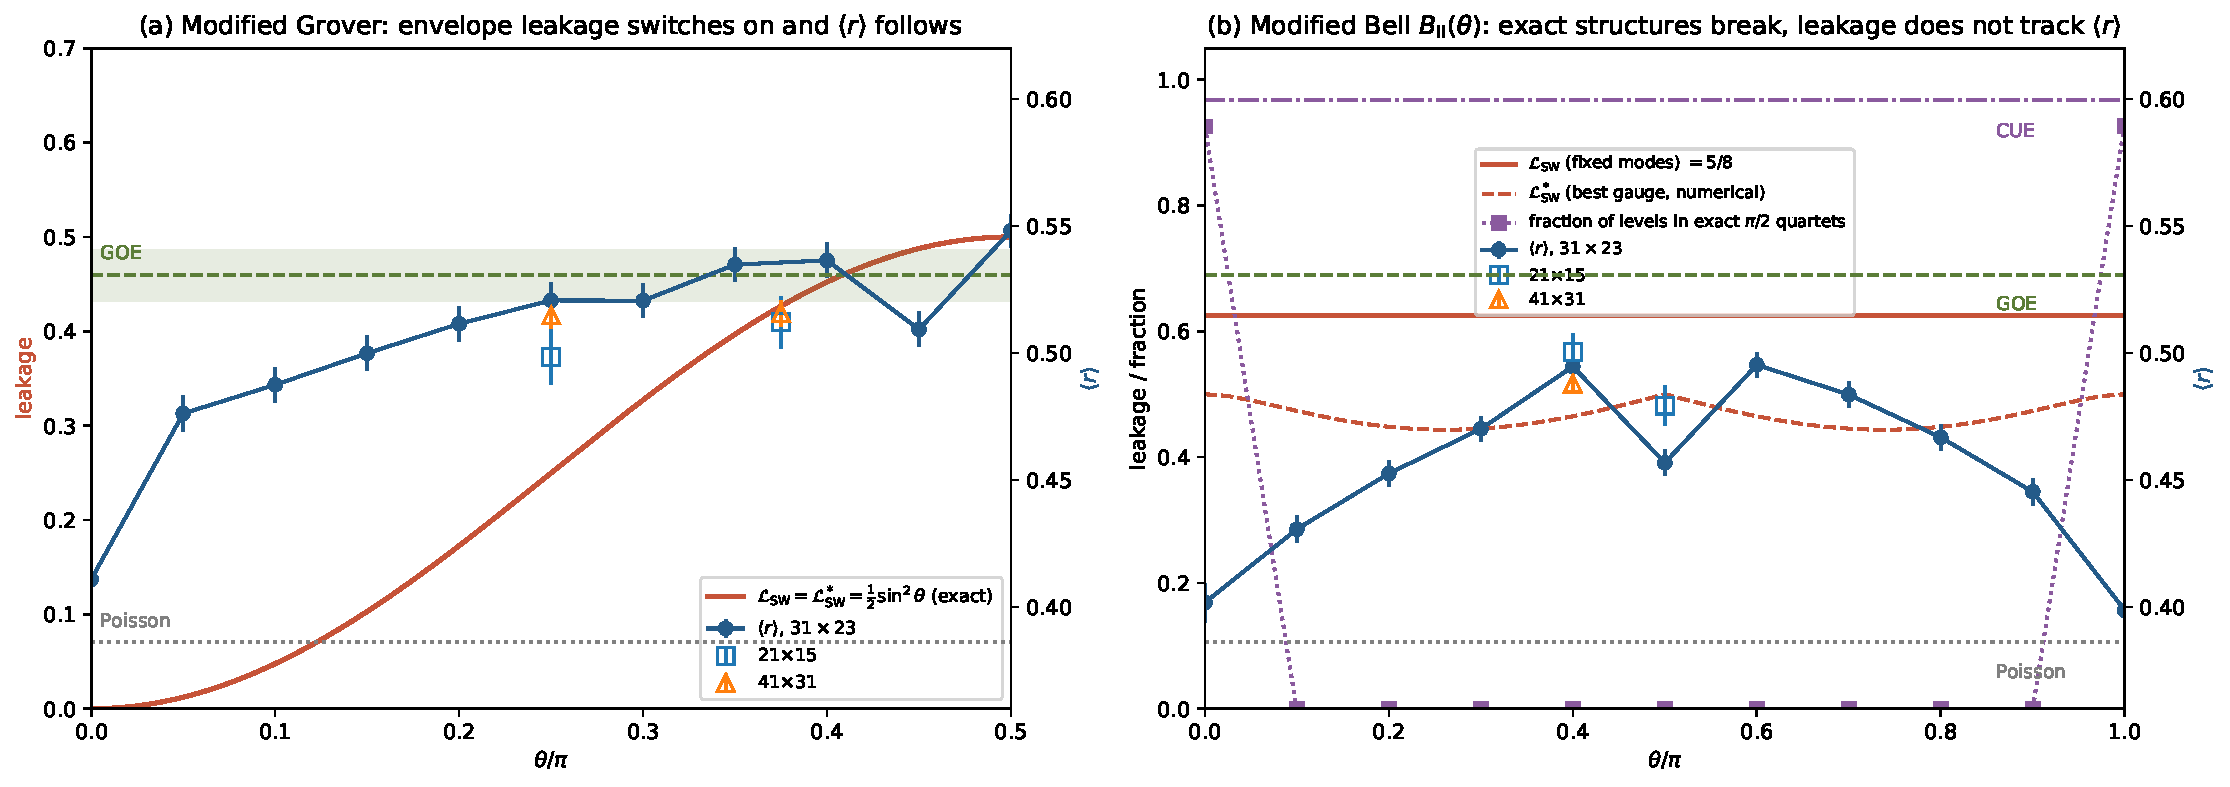
\includegraphics[width=\textwidth]{fig05_mechanisms_leakage_vs_r.pdf}
\caption{(a) Modified Grover: the exact envelope leakage
\(\tfrac12\sin^2\theta\), which equals its gauge minimum, and the
resolved \(\langle r\rangle\) on \(31\times23\), with size checks. The
band is the finite-size GOE null. (b) Modified \(B_{\mathrm{II}}\): the
fixed-mode leakage is constant at \(5/8\); the numerical gauge minimum
stays between \(0.444\) and \(0.5\); the fraction of levels in exact
\(\pi/2\) quartets drops from \(0.93\) to zero for every interior
\(\theta\); \(\langle r\rangle\) stays between the Poisson and orthogonal
values.}
\label{fig:mechanisms}
\end{figure}

\section{A common language, not yet a common mechanism}

All the routes can be written in one language. Every demonstrated
solvable family is a label algebra supplied by the geometry and the
shift, and integrability is broken \emph{within that family} when the
coin makes \(U\) leak out of the algebra. What differs between the
routes is which algebra is lost:
\begin{itemize}
\item modified Grover loses the standing-wave algebra and all its gauge
images;
\item the near-monomial family loses the position--direction basis;
\item \(C_{\mathrm{rot}}\) loses the row/column algebra;
\item modified Bell loses an unidentified structure, visible in the
spectrum as quartets and pairing.
\end{itemize}
The spectral outcomes also differ. The first two reach
orthogonal-class-like local statistics at strong deformation; the last
two stay intermediate at the tested sizes.

\open Whether these are different mechanisms, or one mechanism seen
through different algebras, is left for future work. The question is
whether there is a single structure, fixed by the rectangle and the
shift, whose loss underlies every route. Candidates suggested by the
existing tools are the common commutant \(\mathcal Z_{S,C}\) and a label
algebra larger than the four listed. Natural first steps, \emph{not
attempted in this revision}, are:
\begin{enumerate}
\item compare \(\dim\mathcal Z_{S,C}\) along each deformation at small
sizes;
\item identify the operator or algebra behind \(B_{\mathrm{II}}\)'s
\(\pi/2\) quartets and corner states;
\item test whether \(\langle r\rangle\) along each route tracks the
escape \(\mathcal M^{\mathrm{alg}}\) of the algebra that route destroys.
\end{enumerate}

\begin{lesson}{What the 16-cell map does and does not tell us}
The map tells us, coin by coin and before diagonalizing anything,
whether the rectangle's standing waves survive. In a gauge-adjusted form
it also detects hidden standing waves, as for the compass Fourier coin.
It explains precisely why the Grover rotation breaks integrability, and
why the same rotation applied to \(B_{\mathrm{II}}\) does not act through
that structure. It does not detect other exact structures, such as
routing, independent axes or whatever organizes \(B_{\mathrm{II}}\), and
no leakage value sets a universal threshold for chaotic statistics.
\end{lesson}


\appendix
\chapter{Gauge-equivalent walks and the limits of fixed-mode leakage}
\label{app:gauge}

\section{The verified two-phase equivalence}

The moving shift has an established gauge freedom. Define
\begin{align}
D_{\alpha\beta}
&=\diag(e^{-i\alpha/2},e^{i\alpha/2},
e^{-i\beta/2},e^{i\beta/2}),\\
W\ket{x,y,d}&=e^{i(\alpha x+\beta y)}D_{dd}\ket{x,y,d}.
\end{align}
For a homogeneous coin,
\begin{equation}
\boxed{W U_C W^\dagger=U_{\bar D C\bar D}.}
\label{eq:gauge}
\end{equation}
On an allowed step the position phase supplies the corresponding
opposite-direction phase. At a blocked step the position is unchanged
and \(D_{\bar d\bar d}=\bar D_{dd}\), giving the same identity.
Changing the sign of the parameters shows that \(C\) and \(DCD\)
give unitarily equivalent full walks. This is a congruence of the
coin, realized as a similarity of the walk.

If \(P_a\) are conserved by \(U_C\), the transformed projectors
\(WP_aW^\dagger\) are conserved by its gauge image. A fixed choice
of untransformed modes can therefore report leakage in an exactly
solvable walk.

\section{A counterexample at the same leakage as the modified Grover coin}

The already verified example uses
\begin{equation}
D_\phi=\diag(e^{i\pi/4},e^{-i\pi/4},1,1),\qquad
C'=D_\phi G D_\phi.
\end{equation}
Its fixed-mode leakage is \(3/8\), the same as \(C_G(\pi/3)\),
but with
\begin{equation}
W\ket{x,y,d}=e^{i\pi x/2}(D_\phi)^*_{dd}\ket{x,y,d}
\end{equation}
one has \(U_{C'}=WU_GW^\dagger\). It has exactly Grover's spectrum
and an explicitly transformed complete mode family. This is an exact
counterexample to a universal chaos threshold based on
\(\mathcal L_{\sw}\) alone.

The gauge-adjusted version is
\begin{equation}
\boxed{
\mathcal L^*_{\sw}(C)=
\min_{D=\diag(e^{ia},e^{-ia},e^{ib},e^{-ib})}
\mathcal L_{\sw}(DCD).
}
\end{equation}
It tests membership in the gauge orbit of the specified standing-wave
family. A numerical minimizer gives an upper bound on the true minimum.
A positive value found numerically is not a proven global lower bound.

\section{The established exact minimum for modified Grover}

The supplied teaching source contains the prior exact derivation
\begin{equation}
\boxed{\mathcal L^*_{\sw}(C_G(\theta))=\tfrac12\sin^2\theta.}
\end{equation}
For completeness, put \(u=\sin^2a\), \(v=\sin^2b\), and
\(t=\cos^2\theta\). The retained weight in
Eq.~\eqref{eq:closedleak} after the gauge is
\begin{equation}
F=4(1-\mathcal L_{\sw}(DCD))
=2+2t-2(1+t)(u+v)+2t(u^2+v^2)+(4-2t)uv.
\end{equation}
It is separately convex in \(u,v\in[0,1]\), so a maximum occurs at
a vertex. The four values are \(2+2t,2t,2t,2\), proving the result.
This exact proof belongs to the prior project work; no new minimum
search was performed for these notes.

The Hadamard-per-axis coin \(H\oplus H\), with
\(H=\left(\begin{smallmatrix}1&1\\1&-1\end{smallmatrix}\right)/\sqrt2\),
has fixed leakage \(1/2\) but gauge-minimized leakage zero.
The choice \(a=b=\pi/4\) makes its coherent matrix diagonal.
Thus independent-axis structure and gauge-transformed mode structure
can overlap as solvable families.

\section{An exactly solvable coin with half its weight in forbidden cells}

The compass Fourier coin is a second, simpler example of the same point.
Its fixed-mode forbidden weight is \(\mathcal L_{\sw}(F_c)=1/2\), because
it exchanges \(v_+\) with \(h_-\). With \(D=\diag(i,-i,1,1)\), however,
\(\widetilde{DF_cD}=(i\sigma_x)\oplus(-1)\oplus(i)\) has no forbidden
weight. The gauge transformation
\(W\ket{x,y,d}=(-1)^x\diag(-i,i,1,1)_{dd}\ket{x,y,d}\), which is the case
\(\alpha=\pi\), \(\beta=0\) of Eq.~\eqref{eq:gauge}, maps the walk
exactly onto the transformed one (Section~\ref{sec:fourierfull}). This
supplies the explicit transformation that the earlier record had
identified only numerically.

\section{Four demonstrated reductions, not a classification theorem}

The project has explicit solvability arguments for:
\begin{enumerate}
\item independent homogeneous one-dimensional rows and columns when
\(C=C_H\oplus C_V\);
\item fixed standing-wave blocks for
\(\widetilde C=C_+\oplus e^{i\alpha}\oplus e^{i\beta}\);
\item gauge images of the second family, for example the compass Fourier coin;
\item position--direction routing for monomial coins.
\end{enumerate}
They need not be disjoint, and they have not been proved exhaustive.
For independent rows and columns the block sizes grow with a side
length, and the reduction is to separate one-dimensional problems;
for the standing-wave family the blocks have size at most four.


\chapter{Advanced symmetry and mode diagnostics already established}
\label{app:advanced}

This appendix collects tools from the existing project that are useful
after the first teaching sequence. They generalize the simple leakage
without turning it into a universal chaos criterion.

\section{Allowing deterministic relabeling of sectors}

Equation~\eqref{eq:leakage} vanishes only if each sector keeps its
original label. To accept deterministic exchanges of sectors, use
\begin{equation}
\boxed{
\mathcal L^{\mathrm{route}}_{\mathscr P}(U)
=1-\frac1D\max_{\substack{\pi\ \mathrm{permutation}\\r_{\pi(a)}=r_a}}
\sum_a\norm{P_{\pi(a)}UP_a}_F^2.
}
\end{equation}
Its zero is equivalent to \(UP_aU^\dagger=P_{\pi(a)}\) for an
equal-rank permutation. The sum of projectors around a routing cycle
is conserved. For the two equal-rank coin groups,
\(\mathcal L_q^{\mathrm{route}}=\mathcal M_q/2\).

The earlier restricted summary
\(\min(\mathcal L_{\sw}^{\mathrm{route}},
\mathcal L_{\mathrm{basis}}^{\mathrm{route}})\)
recognized two particular reductions. Enlarging the specified family
to include rows/columns and gauge images is meaningful, but a positive
minimum excludes only the tested reductions.

\section{One formula for the escape of a label algebra}

For \(m>1\) complete sector projectors, define the algebra of
observables constant inside each sector and its normalized basis:
\begin{equation}
\mathcal A_{\mathscr P}=\spanof\{P_a\},\qquad
B_a=P_a/\sqrt{r_a},\qquad
\mathbb E_{\mathscr P}(X)=\sum_a\frac{\Tr(P_aX)}{r_a}P_a.
\end{equation}
The map \(\mathbb E\) replaces each diagonal block by its average;
it differs from retaining the entire block \(\sum_aP_aXP_a\).
Conjugation \(X\mapsto UXU^\dagger\) compressed to the label algebra
has matrix
\begin{equation}
\mathsf K_{ba}=\Tr(B_bUB_aU^\dagger)
=\frac{W_{ba}}{\sqrt{r_br_a}}.
\end{equation}
The established unified diagnostic is
\begin{equation}
\boxed{
\mathcal M^{\mathrm{alg}}_{\mathscr P}(U)
=\frac{m-\norm{\mathsf K}_F^2}{m-1}
=\frac1{m-1}\sum_a
\norm{(1-\mathbb E_{\mathscr P})(UB_aU^\dagger)}_F^2.
}
\end{equation}
It lies in \([0,1]\). Its zero is exactly the routing condition
\(UP_aU^\dagger=P_{\pi(a)}\) with equal ranks. The reason is that
zero escape makes conjugation an automorphism of this commutative
algebra, and such an automorphism permutes its minimal projectors.
No assignment optimization is needed for this test.

For the binary groups it reduces to
\begin{equation}
\mathcal M_q^{\mathrm{alg}}=4p(1-p)
=\mathcal M_q(2-\mathcal M_q).
\end{equation}
For the rank-one position--direction basis it becomes
\begin{equation}
\mathcal M^{\mathrm{alg}}_{\mathrm{basis}}(U)
=\frac{D-\sum_{i,j}|U_{ij}|^4}{D-1},
\end{equation}
which vanishes for precisely the monomial unitaries. For Grover,
choosing the standing-wave projectors instead gives zero. Its
normalization averages label observables, rather than the state
probabilities used by \(\mathcal L\); nonzero values need not agree.

This is an application of established coherence-generation and
algebra-overlap constructions \cite{cgp,alggeom,gaac}, not a claimed
new universal detector. With \(\mathcal B=\mathcal A_{\mathscr P}'\),
it equals \(m/(m-1)\) times the geometric algebra anti-correlator
\(G_{\mathcal B}(U)\) used in the earlier report.

\section{Finding the part of a mode structure that survives}

If \(\mathsf K z=\mu z\) with \(|\mu|=1\), then
\begin{equation}
Q_z=\sum_a z_aB_a\quad\Longrightarrow\quad
UQ_zU^\dagger=\mu Q_z.
\end{equation}
Projection cannot increase the Hilbert--Schmidt norm. Equality of
the full and compressed norms for this eigenvector forces the
component outside the label algebra to vanish. In particular,
\(\mu=1\) identifies an exactly conserved observable.
A singular value one alone only gives a one-step statement, not
persistent invariance of an observable.

Equivalently, for real \(q_a\) and \(Q(q)=\sum_aq_aP_a\),
\begin{align}
\norm{[U,Q(q)]}_F^2
&=\sum_{a,b}(q_a-q_b)^2W_{ba}\\
&=2q^{\mathsf T}
\left[\diag(r)-\frac{W+W^{\mathsf T}}2\right]q.
\end{align}
Connect labels whenever \(W_{ab}+W_{ba}>0\). Conserved \(q\)'s
are precisely those constant on each connected component. On the
recorded \(9\times7\) example there are 79 standing-wave sectors.
Grover leaves all 79 isolated. At \(C_G(\pi/3)\) there are three
components: \(\mathcal K_{00}\), the rest of the even rotation
sector, and the odd rotation sector. Large invariant components do
not solve their internal dynamics.

The matrix \(W_{ba}/r_a\) has a one-step probability interpretation.
Its powers do not generally give the unmeasured quantum evolution of
sector probabilities: the compression discards coherences that can
later return.

\section{A systematic search for common conserved observables}

The shift commutant and the common commutant are
\begin{equation}
\mathcal B_S=\{X:[X,S]=0\},\qquad
\mathcal Z_{S,C}=\{X:[X,S]=[X,\CC]=0\}.
\end{equation}
In an orthonormal operator basis \(E_\alpha\) of \(\mathcal B_S\),
the positive matrix
\begin{equation}
H_{\alpha\beta}=\frac14\Tr\left(
[\CC,E_\alpha]^\dagger[\CC,E_\beta]\right)
\end{equation}
has a kernel giving exactly \(\mathcal Z_{S,C}\), because its
quadratic form is \(\norm{[\CC,X]}_F^2/4\). Its eigenvalues lie in
\([0,1]\). The identity is always a trivial conserved element.
This includes coherences outside the standing-wave label algebra.
The prior finite \(4\times3\) check found
\(\dim\mathcal B_S=216\) and
\(\dim\mathcal Z_{S,C_G(\pi/3)}=6\).
These numbers are not an all-size theorem. A symmetry of the product
need not commute with its factors separately, so this search does
not exhaust every possible full-walk symmetry.

\section{Uniform and checkerboard subspaces}

The supplied teaching source also established the following simple
spaces. Define
\begin{equation}
\ket u=N^{-1/2}\sum_{x,y}\ket{x,y},\qquad
\ket\chi=N^{-1/2}\sum_{x,y}(-1)^{x+y}\ket{x,y}.
\end{equation}
The shift is \(+1\) on
\(\ket u\otimes\spanof\{h_+,v_+\}\) and \(-1\) on
\(\ket\chi\otimes\spanof\{h_-,v_-\}\).
For the second space an interior move changes the checkerboard sign,
whereas a wall reversal changes the antisymmetric direction sign.
Both give the same factor \(-1\).

Whenever \([C,J]=0\), its coherent matrix is
\(\widetilde C=C_+\oplus C_-\). The two displayed spaces remain
invariant under the full walk, with restricted matrices \(C_+\) and
\(-C_-\). For modified Grover they supply eigenvalues
\begin{equation}
\boxed{+1,-1,e^{i\theta},e^{-i\theta}.}
\end{equation}
The checkerboard projector generally has off-diagonal terms between
the terminal standing-wave sectors, explaining why a graph of the
original diagonal labels does not find it. These special states still
leave an extensive unresolved space.

\section{General reversing and spectral-equivalence tests}

For a corresponding pair
\begin{equation}
(P,\sigma)\in
\{(\mathcal J,J),(\mathcal P_x\mathcal J,\sigma_y),
(\mathcal P_y\mathcal J,\sigma_x),(\mathcal R\mathcal J,\Id)\},
\end{equation}
one has \(PSP=S^{-1}\). If \(\sigma C\sigma=C^{\mathsf T}\),
then the verified sufficient construction is
\begin{equation}
A=\CC^\dagger PK,\qquad AUA^{-1}=U^{-1},\qquad A^2=\Id.
\end{equation}
Other established comparisons are
\begin{equation}
\spec U_C=\spec U_{JC^{\mathsf T}J},\qquad
U_{\bar C}=\overline{U_C}.
\end{equation}
A scalar coin phase rotates the quasienergies uniformly. These are
useful comparisons of walks; they should not be confused with a
complete list of their commuting symmetries.

\section{Why small leakage alone does not set a crossover scale}

The prior perturbative discussion used
\(U_G(\theta)=U_G(0)e^{-i\theta(\Id\otimes V)}\).
For nondegenerate Grover eigenstates \(a,b\), a first-order
hybridization indicator was
\begin{equation}
\kappa_{ab}(\theta)=
\frac{|\theta\langle a|\Id\otimes V|b\rangle|}
{2|\sin[(\varphi_a-\varphi_b)/2]|}.
\end{equation}
The numerator must be compared to a symmetry-allowed phase separation,
not only to one. Grover's extensive degenerate subspaces require
degenerate perturbation theory instead. The retained mode-overlap
selection rule can connect many labels, with an approximate overlap
\(\langle f_p,g_m\rangle\simeq(4/\pi)m/(m^2-p^2)\) in the regime
tested in the export. It is not an exact finite-size identity.

Thus loss of exact mode conservation at any nonzero allowed coupling
and the appearance of a random-matrix-like spectral window are
different statements. No universal crossover scale was established.

Nor can unrestricted optimization over all mode bases repair this:
every finite unitary has rank-one eigenprojectors with zero leakage.
The tested family must be constructed from the geometry or another
independently specified structure. This is why the common algebra
formula still needs its family of labels.

\section{The wall-reflection pre-test and its limited scope}

The retained bulk equation is \(U(k_x,k_y)u=\lambda u\).
At fixed \((k_y,\lambda)\),
\(z\det[\lambda\Id-U(k_x,k_y)]\), \(z=e^{ik_x}\), is a
polynomial of degree at most two. The determinant may vanish
identically on a flat band, roots may coincide, and a root need not
be a propagating real wavevector. The regular two-wave interpretation
requires these exceptional cases to be excluded.

For a superposition of bulk waves the actual right-wall equation is
\begin{equation}
\sum_jA_j e^{ik_jN_x}
\big[(Cu_j)_R-e^{ik_j}(Cu_j)_L\big]=0.
\end{equation}
The top wall replaces \((R,L,k,N_x)\) with \((U,D,q,N_y)\).
At a regular band point these equations define partner waves and
reflection amplitudes. If horizontal and vertical reflection paths
close on the same four-wave set, their consistency requires
\begin{equation}
K_{\mathrm{corner}}
=\frac{r_x(q)r_y(k')}{r_y(k)r_x(q')}=1.
\end{equation}
When closure holds, eigenvector phase and wall-position factors cancel
from the ratio. The retained tests find closure and unit corner phase
for Grover and the tested gauge images; modified Grover at generic
interior parameters fails closure. At \(\pi/2\) it closes but has
corner phase \(-1\). The real-generator variant below closes at the
tested points but has a nonunit corner phase.

This tests a particular four-wave ansatz. It is not a complete
integrability criterion: routing-solvable permutations can fail it,
and independent row/column walks can make it undefined. An orbit
not closing within 800 tested reflections is not a proof of an
infinite orbit. The proposed ray interpretation was untested and is
not used to classify the walks here.


\chapter{Supplementary verified examples and numerical records}
\label{app:additional}
\label{app:record}

The following material is retained for a second reading. It records
already completed work, not additional computations for these notes.
Finite numerical observations keep their original limitations.

\section{A position-only description of the Grover spectrum}

The Grover-billiard export also established a smaller real symmetric
matrix. Let \(A\ket{\mathbf r}=\ket{\mathbf r}\otimes\ket s\),
where \(\ket s=(1,1,1,1)^{\mathsf T}/2\), and let
\(S_{\mathrm{ff}}\) have the older flip-flop/self-loop convention.
Then
\begin{equation}
T=A^\dagger S_{\mathrm{ff}}A
=\frac{\operatorname{Adj}+\diag(\text{missing-neighbor counts})}{4}.
\end{equation}
This is a matrix of nearest-neighbor averages with missing links
replaced by staying at the site. It is an auxiliary spectral matrix,
not the walker Floquet operator. For the rectangle,
\begin{equation}
T=\frac12(T_x\otimes\Id_y+\Id_x\otimes T_y),\qquad
\mu_{mn}=\frac12\left(\cos\frac{\pi m}{N_x}
+\cos\frac{\pi n}{N_y}\right).
\end{equation}
Its eigenvectors are products of the cosine profiles. For the moving
Grover walk, the dispersive phases satisfy
\(\cos\varphi_{mn}=-\mu_{mn}\), agreeing with
Eq.~\eqref{eq:groverspectrum}; the extensive flat subspaces must still
be added. For \(Tf=\mu f\), \(-1<\mu<1\), put
\(\lambda=\mu+i\sqrt{1-\mu^2}\) and
\(\mathcal Q=\Id\otimes(J\Gamma)\). The recorded full-state
construction is
\begin{equation}
\phi=\mathcal Q(Af-\lambda S_{\mathrm{ff}}Af),\qquad
U_G\phi=-\lambda\phi.
\end{equation}
It is written before normalization; the partner branch is obtained
from the conjugate eigenvalue. The export verified this construction
with residual at most \(7.6\times10^{-16}\) on \(7\times5\).
For a nonsquare rectangle its parity labels agree with those of the
scalar reduction. On a square, the recorded moving-Grover
\(D_4\) correspondence exchanges \(A_1\leftrightarrow B_1\) and
\(A_2\leftrightarrow B_2\) between the scalar and Floquet descriptions,
while retaining \(E\). These labels must therefore be assigned using
the physical full-walk symmetry projectors.

This reduction and the explicit four-dimensional mode blocks are two
consistent descriptions of the same rectangular Grover solution.
They should not be extended to arbitrary coins by analogy.

\subsection{The special verified correspondence between the two shifts}

The Grover-billiard export gives a stronger statement for \(G\).
With \(\mathcal Q=\Id_{\mathrm{pos}}\otimes(J\Gamma)\),
\begin{equation}
\boxed{U_{\mathrm{mov},G}=-\mathcal Q
U_{\mathrm{ff},G}\mathcal Q^\dagger.}
\end{equation}
Thus the dispersive phases map by
\(\varphi_{\mathrm{mov}}=\pi-\varphi_{\mathrm{ff}}\) on the
positive branch, and the \(\pm1\) multiplicities exchange.
For the rectangle the moving-shift multiplicities are those in
Chapter~\ref{ch:assembled}; the flip-flop ones are the reverse.
This is a verified Grover-specific correspondence, not a license to
transfer arbitrary fixed-coin numerical results between shifts.

\section{Square controls and representation dimensions}

The square is a special rectangle. For Grover it has the full
\(D_4\) geometry, whose irreducible representation dimensions are
\(1,1,1,1,2\), commonly labeled \(A_1,A_2,B_1,B_2,E\).
A two-dimensional irrep can occur many times. Its isotypic subspace
contains a repeated symmetry copy of each associated eigenvalue; one
row of the irrep is used for an independent spacing sequence. For
example, in the recorded \(60\times60\) Grover calculation the
dispersive \(E\) row contains 900 levels. Calling \(E\) a
two-dimensional representation does not say the full sector contains
only two states.

Modified Grover generally retains a smaller square group generated by
\(\mathcal R\) and diagonal reflection \(\Sigma\):
\(\{\Id,\mathcal R,\Sigma,\mathcal R\Sigma\}\). On
\(23\times23\) its four joint sectors have dimension 529.
The source's control is
\begin{center}
\small
\begin{tabular}{@{}lll@{}}
\toprule
Parameter&Only rotation resolved&Four joint sectors resolved\\
\midrule
\(\theta=\pi/3\)&0.3644, 0.3741&0.5330, 0.5266, 0.5371, 0.5149\\
\(\theta=\pi/2\)&0.4191, 0.4213&0.5288, 0.5288, 0.5295, 0.5283\\
\bottomrule
\end{tabular}
\end{center}
These are different symmetry resolutions, not contradictory spectra.
Independent random superposition models are only comparison references
for symmetry sectors that may be correlated in the deterministic walk.

\section{The real-generator variant and the independent-axis family}

The real variant of modified Grover has coherent matrix
\begin{equation}
\widetilde C'(\theta)=
\begin{pmatrix}0&1\\1&0\end{pmatrix}
\oplus
\begin{pmatrix}-\cos\theta&\sin\theta\\
-\sin\theta&-\cos\theta\end{pmatrix}.
\end{equation}
It is real but generally nonsymmetric. It has the same fixed-mode
leakage \(\frac12\sin^2\theta\), survives rotation, and satisfies
\(\sigma_yC'\sigma_y=C'^{\mathsf T}\), giving time reversal via
\(\mathcal P_x\mathcal J\). The recorded half-circle means on
\(25\times19\) at \(\pi/3\) are \(0.525,0.536\). The earlier
prediction of a unitary-class benchmark from its nonsymmetry was
retracted after this reversing relation was found.

For another deterministic construction, set
\begin{equation}
R_\eta=\begin{pmatrix}\cos\eta&-\sin\eta\\
\sin\eta&\cos\eta\end{pmatrix},\qquad
B_\eta=R_\eta\oplus R_\eta,\qquad\eta=\pi/4,
\end{equation}
and use the permutation \(P\) from Chapter~\ref{ch:coins}. The
recorded family is
\begin{equation}
C_{\mathrm{rot}}(\varphi)
=B_\eta e^{-i\varphi P}.
\end{equation}
At zero it preserves independent rows and columns. It leaves that
specified decomposition with exact leakage
\(\mathcal L_{\rc}=\sin^2\varphi\). Its pair vector is
\begin{equation}
\bigl(2\min(\cos^2\varphi,\sin^2\varphi),1,1\bigr).
\end{equation}
The starting coin has \(\mathcal L^*_{\sw}=1/2\), so it supplies
a genuinely different tested reduction from gauge-transformed
standing waves. At general parameter the ordinary rotation does not
survive, but \(JCJ=C^{\mathsf T}\) gives time reversal and
\(\Gamma\bar C\Gamma=C\) gives a commuting antiunitary.
An additional anticommuting operator was found in the source search.
No complete symmetry classification was obtained.

The recorded comparison uses half circles, with rotation sectors
resolved for modified Grover:
\begin{center}
\small
\begin{tabular}{@{}lrrrrrr@{}}
\toprule
&\multicolumn{2}{c}{\(25\times19\)}&\multicolumn{2}{c}{\(29\times18\)}
&\multicolumn{2}{c}{\(40\times13\)}\\
Parameter&\(C_G\)&\(C_{\mathrm{rot}}\)&\(C_G\)&\(C_{\mathrm{rot}}\)
&\(C_G\)&\(C_{\mathrm{rot}}\)\\
\midrule
0.05&0.443&0.441&0.465&0.443&0.485&0.448\\
0.10&0.474&0.446&0.473&0.443&0.508&0.488\\
0.30&0.502&0.446&0.511&0.436&0.536&0.474\\
0.60&0.519&0.428&0.521&0.413&0.528&0.441\\
1.25&0.511&0.393&0.535&0.370&0.522&0.391\\
\bottomrule
\end{tabular}
\end{center}
Over the source's 12 points in \([0.6,1.3]\), its recorded aggregate
means were \(0.5261\) for modified Grover and \(0.4160\) for the
rotation family. The latter does not prove integrability or imply
that an unidentified conserved quantity must exist.

\section{Other explicitly tested deterministic constructions}

To preserve the candidate-search record without replacing the main
examples, the following definitions are retained. The Fourier-based
constructions of the earlier record (fractional Fourier powers and the
designed Fourier family) are removed from these notes. Put
\(E(a,b)=\ket a\bra b+\ket b\bra a\),
\(Y=E(R,D)+E(L,U)\), and the signed turn
\(X_F=E(R,U)-E(L,D)\), with \(X_F^2=\Id\).
For two-dimensional blocks let
\begin{equation}
K(\eta,\xi)=e^{i\eta\sigma_x/2}R_\xi e^{i\eta\sigma_x/2},
\qquad \sigma_x=\begin{pmatrix}0&1\\1&0\end{pmatrix}
\end{equation}
in this formula only. It is a block Pauli matrix, not the full
four-direction reflection symbol used elsewhere.

\begin{center}
\small
\begin{tabularx}{\textwidth}{@{}lY@{}}
\toprule
Source label&Retained definition\\
\midrule
\(C_x(\varphi)\)&\(e^{-i\varphi Y/2}B_{\pi/4}e^{-i\varphi Y/2}\)\\
\(C_n(\varphi)\)&\(e^{-i\varphi Y/2}[K(\pi/3,\pi/4)\oplus K(\pi/3,\pi/4)]e^{-i\varphi Y/2}\)\\
\(C_m(\varphi)\)&Same sandwich, with blocks \(K(\pi/3,\pi/4)\) and \(K(\pi/5,0.9)\)\\
Direction hopping A&\(\exp[-i(P+0.6Y+0.8\Gamma)]\)\\
Direction hopping B&\(\exp[-i(P+0.6Y+0.8\Gamma+0.5X_F)]\)\\
Near-monomial&\(e^{-i\epsilon H/2}P e^{-i\epsilon H/2}\),
\(H=X_F+0.7Y+0.4\Gamma+0.3E(R,L)\)\\
\bottomrule
\end{tabularx}
\end{center}
Selected recorded observations are:
\begin{center}
\small
\begin{tabularx}{\textwidth}{@{}llY@{}}
\toprule
Family&Setting&Recorded \(\langle r\rangle\) and scope\\
\midrule
\(C_x\)&\(\varphi=0.4,0.8,1.2\)&0.418, 0.443, 0.485 on \(25\times19\) (session-only)\\
\(C_n\)&Same parameters&0.407, 0.439, 0.446 on \(25\times19\) (session-only)\\
\(C_m\)&Same parameters&0.466, 0.469, 0.431 on \(25\times19\) (session-only)\\
Direction hopping A&\(25\times19\), rotation sectors&0.499, 0.496\\
Direction hopping B&\(25\times19\)&0.500\\
Near-monomial&\(\epsilon=0.02,0.2,0.8\)&0.18, 0.35, 0.517 on \(25\times19\)\\
\bottomrule
\end{tabularx}
\end{center}
These are finite candidate tests, not a classification or a universal
threshold. Exact monomial coins were
verified to have one nonzero entry per full-walk column, consistent
with the exact routing proof.

\section{Aspect ratios, special phases, and distribution tests}

The modified-Grover aspect sweep used 33 parameter values and the
five rectangles in the next table. Its plateau summary averages
\(\theta\in\{0.6,0.8,\pi/3,1.25\}\):
\begin{center}
\begin{tabular}{@{}lrrr@{}}
\toprule
Rectangle&Aspect ratio&Plateau mean&SD across four parameters\\
\midrule
\(25\times19\)&1.32&0.5140&0.0032\\
\(29\times18\)&1.61&0.5354&0.0110\\
\(33\times16\)&2.06&0.5312&0.0087\\
\(40\times13\)&3.08&0.5287&0.0050\\
\(51\times10\)&5.10&0.5495&0.0112\\
\bottomrule
\end{tabular}
\end{center}
Across these 20 points the recorded average is \(0.5318\), with
SD \(0.0139\). Geometry-dependent offsets of order \(0.01\)--\(0.02\)
were not excluded. At \(\pi/3\), the source's pooled distribution
has \(n=4963\), mean \(0.5360\), and a calibrated COE test
\(p=0.080\); the uncalibrated independent-sample test gave
\(p=0.009\). Its full archive was not attached to the earlier audit
review described in the supplied notes. These are retained as recorded results
of the exported session, not claimed as a fresh independent reproduction.

The suggested \(0.35/\sqrt n\) scale was calibrated on finite COE
simulations. It is not a universal error formula. Taking one conjugate
half removes exact repetitions but does not make neighboring ratios
independent. Full- and half-circle means can differ through endpoint
gaps. No confidence interval is inferred here from the sweep SDs.

The source observed additional degenerate phases away from Grover.
For example, the full-spectrum multiplicity of each of \(\pm1\) at
\(\theta=\pi/3\) was 1 on \(25\times19\), 13 on \(40\times13\),
29 on \(29\times18\), and 42 on \(26\times18\). The general
side-parity pattern was empirical, not proved. At \(\pi/2\),
\(\pm i\) also show parity-dependent degeneracies. A source table
of these special-point means is summarized by the odd-by-odd versus
even-side distinction in the main chapter.

\section{Random coins, flux, and frozen-disorder controls}

The additional Haar-coin study reported four means on \(25\times19\):
\(0.556,0.555,0.520,0.486\), pooled mean \(0.5291\). The coin
generation was complex Gaussian QR with phase correction. Restricted
searches found no time reversal, yet the local ratios were closer
to the orthogonal reference than the unitary reference. This is an
unexplained observation; the searches are not absence proofs.

A flux-control step was specified as
\begin{equation}
U_B=S\,\diag_{x,y,d}(\mathrm{ph})\,[\Id\otimes C_G(\pi/3)],
\qquad
\mathrm{ph}=(e^{iB(y-c)},e^{-iB(y-c)},1,1),
\end{equation}
with \(c=(N_y-1)/2\) in the zero-based implementation. On
\(25\times19\), the recorded sector means were
\((0.527,0.500)\) at \(B=0\),
\((0.551,0.579)\) at \(B=0.05\), and
\((0.552,0.536)\) at \(B=0.2\). Here \(B\) is the phase parameter
as written in the source code, without an added conversion of units.
These samples did not demonstrate unitary-class universality.

Frozen, site-dependent rotation-family coins were also tested on
\(25\times19\), changing the homogeneous model. Random
\(\varphi_{xy}\in[0.3,0.9]\) gave \(0.533\); random
\(\eta_{xy}\in\pi/4\pm0.3\) gave \(0.516\), compared with
\(0.428\) in the homogeneous reference. These are finite-size
controls. They do not establish a thermodynamic delocalized phase,
and the exported discussion explicitly qualified the original
``disorder restores chaos'' interpretation.


\chapter{The older random-coin interpolation uses a different shift}
\label{app:legacy}

This appendix consolidates the two earlier crossover exports. Their
results are useful, but they belong to the flip-flop/self-loop shift
of Chapter~\ref{ch:shift}. They are not moving-shift results for the
same unchanged coin.

\section{A second shift used in the older sessions}

Some exports instead use a flip-flop shift \(S_{\mathrm{ff}}\).
It reverses the direction after an allowed move and keeps the state
unchanged at a missing link. The two conventions are:
\begin{center}
\small
\begin{tabularx}{\textwidth}{@{}lYY@{}}
\toprule
& Moving shift \(S_\Omega\)&Flip-flop shift \(S_{\mathrm{ff}}\)\\
\midrule
Allowed link&\(\ket{\mathbf r,d}\mapsto\ket{\mathbf r+\delta_d,d}\)
&\(\ket{\mathbf r,d}\mapsto\ket{\mathbf r+\delta_d,\bar d}\)\\
Missing link&\(\ket{\mathbf r,d}\mapsto\ket{\mathbf r,\bar d}\)
&\(\ket{\mathbf r,d}\mapsto\ket{\mathbf r,d}\)\\
Square&Generally \(S_\Omega^2\neq\Id\)&\(S_{\mathrm{ff}}^2=\Id\)\\
\bottomrule
\end{tabularx}
\end{center}
The verified relation is
\begin{equation}
S_\Omega=\mathcal J S_{\mathrm{ff}}.
\end{equation}
This does not mean that an arbitrary fixed coin gives the same full
walk under both shifts. The old random-coin interpolation is therefore
kept separate in Appendix~\ref{app:legacy}. A special verified spectral
correspondence for Grover is given in Appendix~\ref{app:additional}.

\begin{lesson}{The historical shift convention is a different model}
``Reflecting boundary'' is insufficient to reconstruct a walk.
The internal direction after an allowed move and after a blocked move
must both be stated. The involution property of the flip-flop shift
must not be assigned to the moving shift.
\end{lesson}



\section{The specified historical model}

The geometry is \(N_x=10,N_y=6\), \(D=240\), with no periodic
boundary. The step is
\begin{equation}
U_{\mathrm{ff}}(\lambda)=S_{\mathrm{ff}}
[\Id_{60}\otimes C(\lambda)].
\end{equation}
The shift satisfies \(S_{\mathrm{ff}}^\dagger=S_{\mathrm{ff}}\),
\(S_{\mathrm{ff}}^2=\Id\), and
\(\Tr S_{\mathrm{ff}}=2N_x+2N_y=32\), the boundary self-loops.
The original coin was a single COE draw \(V^{\mathsf T}V\), with
\(V\) obtained from a seeded complex-Gaussian QR construction,
seed 16. E3 records that seed 16 was selected after scanning seeds
1--30 for proximity to the orthogonal reference. Their recorded mean
was \(0.4884935\), population SD \(0.0371222\), minimum \(0.4132964\)
and maximum \(0.5499779\). The selected \(0.5318896\) is not an
ensemble mean. The preliminary seed-20261001 endpoint was \(0.4181041\)
with the flip-flop shift and \(0.4261382\) in its exploratory
moving-shift test. Those are distinct records, not points on the
seed-16 curve.

The supplied reproduction instead specifies the following
six-decimal real symmetric generator as its numerical input:
\begin{equation}
K_*^{\mathrm{doc}}=
\begin{pmatrix}
1.154349&-0.635057&0.212309&-0.148986\\
-0.635057&0.875129&0.203120&-1.258544\\
0.212309&0.203120&1.490150&1.547436\\
-0.148986&-1.258544&1.547436&-0.761511
\end{pmatrix}.
\end{equation}
The split is
\begin{equation}
K(\lambda)=
\begin{pmatrix}K_H&\lambda W\\\lambda W^{\mathsf T}&K_V\end{pmatrix},
\qquad C(\lambda)=e^{-iK(\lambda)},\qquad0\leq\lambda\leq1,
\end{equation}
where \(K_H,K_V,W\) are the displayed generator's blocks. It
couples the two axis sectors of the \emph{generator}. It is different
from the path \(e^{-i\lambda K_*}\), which scales the whole generator.

The coins are symmetric unitary, and the reproduced full step has
time reversal \(A_{\mathrm{ff}}=S_{\mathrm{ff}}K\), with square one.
At zero the coin is block diagonal in the axes. The row and column
projectors commute with the full step. Its spectrum contains 20
distinct phases repeated six times and 12 distinct phases repeated
ten times in this example, as checked in the reproduction.

\section{The degenerate endpoint and the definition of a ratio mean}

The full zero-coupling spectrum has 208 zero gaps. There are 176
undefined \(0/0\) ratios and 64 ratios equal to zero next to a
nonzero gap. The two exports use different estimators at this point:
\begin{center}
\small
\begin{tabularx}{\textwidth}{@{}lY@{}}
\toprule
Convention&Treatment of the \(\lambda=0\) full spectrum\\
\midrule
Strict formula&The mean including every ratio is undefined\\
Omit undefined ratios&The retained mean is zero (numerical original: about \(7.7\times10^{-14}\))\\
Replace undefined ratios by zero&The zero-filled mean is zero, but this is a different estimator\\
\bottomrule
\end{tabularx}
\end{center}
None is evidence of a Poisson endpoint. Removing \(0/0\) terms is
not symmetry resolution. The degeneracy comes from identical
homogeneous row and column copies.

\section{Recorded positive-coupling values and precision labels}

The original full-precision seeded construction and the reproduction's
six-decimal generator are different specified numerical inputs.
Their small differences are retained rather than silently replacing
one data record by the other:
\begin{center}
\begin{tabular}{@{}lrr@{}}
\toprule
\(\lambda\)&Original seeded path&Six-decimal documented path\\
\midrule
0.02&0.297681&0.297632\\
0.10&0.361189&0.361190\\
0.12&0.393100&0.393099\\
0.20&0.445458&0.445458\\
0.40&0.483130&0.483131\\
0.60&0.483969&0.483968\\
0.80&0.511780&0.511779\\
1.00&0.531890&0.531890\\
\bottomrule
\end{tabular}
\end{center}
No symmetry sectors were resolved in these historical full-circle
values. The reproduction checked the documented path in independent
Python and Octave implementations, with agreement about
\(3\times10^{-12}\) at a representative checkpoint and 56 Octave
assertions passed. The original positive-coupling data are redrawn
below from their retained 51-point CSV. No new spectra are involved.

\begin{figure}[htbp]
\centering
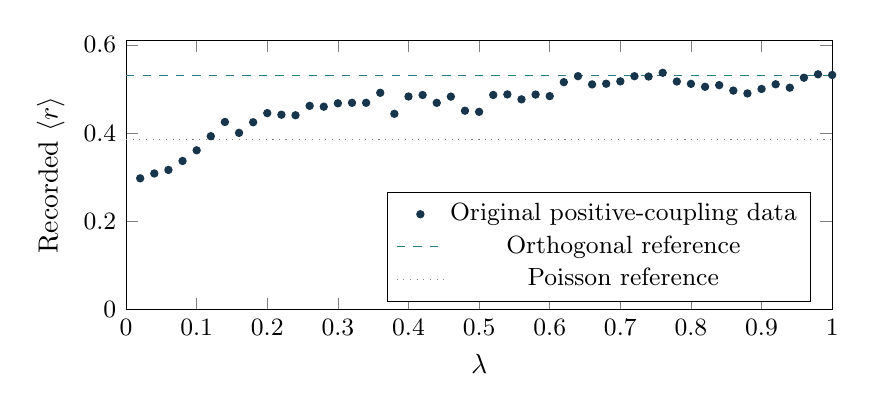
\begin{tikzpicture}
\begin{axis}[width=.87\textwidth,height=5cm,xlabel={\(\lambda\)},
ylabel={Recorded \(\langle r\rangle\)},xmin=0,xmax=1,ymin=0,ymax=.61,
legend style={font=\small,at={(.97,.03)},anchor=south east},
tick label style={font=\small}]
\addplot[ink,only marks,mark=*,mark size=1.3pt] coordinates {
(0.02,0.2976812363462865)
(0.04,0.30874095431803084)
(0.06,0.3166977385994079)
(0.08,0.337016998310286)
(0.1,0.3611886289190379)
(0.12,0.3930995243146621)
(0.14,0.42538711449693495)
(0.16,0.40069506828473195)
(0.18,0.42478298579878326)
(0.2,0.44545759359999987)
(0.22,0.4418306723246534)
(0.24,0.4405950214558406)
(0.26,0.4619791575660486)
(0.28,0.4600486534461375)
(0.3,0.467682015831494)
(0.32,0.46874169834822543)
(0.34,0.4688627151920117)
(0.36,0.49153032907412825)
(0.38,0.4439105294405451)
(0.4,0.48312981093765556)
(0.42,0.4864923694218932)
(0.44,0.46874325609006046)
(0.46,0.4828379286999788)
(0.48,0.4508674231039253)
(0.5,0.4483276858892045)
(0.52,0.4865898871036129)
(0.54,0.48785016354232413)
(0.56,0.47664864149992886)
(0.58,0.48752325940560687)
(0.6,0.4839692008645776)
(0.62,0.5155856050419294)
(0.64,0.5292071104486022)
(0.66,0.5105325501274833)
(0.68,0.5121014936939354)
(0.7000000000000001,0.5174020335972777)
(0.72,0.5291066304070401)
(0.74,0.5283719322428141)
(0.76,0.536854253807584)
(0.78,0.5170785051563669)
(0.8,0.5117798879031086)
(0.8200000000000001,0.5051190997708862)
(0.84,0.508854043829866)
(0.86,0.49648031169562246)
(0.88,0.49008165078200017)
(0.9,0.500211951852327)
(0.92,0.5108332535415967)
(0.9400000000000001,0.5030742422448834)
(0.96,0.5256829975183492)
(0.98,0.5333912224251764)
(1.0,0.5318895918770428)};
\addlegendentry{Original positive-coupling data}
\addplot[accent,dashed,domain=0:1]{.5307};
\addlegendentry{Orthogonal reference}
\addplot[gray,dotted,domain=0:1]{.386294};
\addlegendentry{Poisson reference}
\end{axis}
\end{tikzpicture}
\caption{The historical \(10\times6\) flip-flop/self-loop walk,
redrawn from the original exported CSV. Only positive coupling is
shown; its degenerate zero-coupling spectrum needs the estimator
qualification in the text. This is not the main moving-shift model.}
\end{figure}


These data demonstrate a degenerate decomposable endpoint and
orthogonal-class-like local means for one finite realization, not a
universal Poisson-to-COE crossover. The disputed alternative plot was
not reproduced by this model, a whole-generator scaling, or periodic
boundaries. A consistent change of site-index order cannot change
eigenphases. The special correspondence for Grover between the two
shifts is given in Appendix~\ref{app:additional}.

\chapter{Source inventory, consistency decisions, and remaining limits}
\label{app:sources}

\section{Sources and their distinct roles}

The supplied set contains five distinct Markdown exports, one teaching
source and two distinct PDFs. Three pairs of export files and the two
teaching-PDF copies are byte-identical. Duplicate attachments are not
independent replications.
\begin{longtable}{@{}>{\raggedright\arraybackslash}p{.08\textwidth}>{\raggedright\arraybackslash}p{.43\textwidth}>{\raggedright\arraybackslash}p{.41\textwidth}@{}}
\toprule Source & Attached filename & Role\\\midrule\endfirsthead
\toprule Source & Attached filename & Role\\\midrule\endhead
E1 & \nolinkurl{DQW_chat_complete_export (1).md}
& Original \(10\times6\) flip-flop interpolation, complete CSV and estimator\\
E2 & \nolinkurl{DQW_session_export(1).md}
& Rectangle audit: coins, exact modes, diagnostics, modified Grover, designed Fourier and numerical qualifications\\
E3 & \nolinkurl{DQW_this_chat_self_contained_export (1).md}
& Earlier interpolation including the 30-seed scan, seed selection and preliminary moving-shift run\\
E4 & \nolinkurl{DQW_chat_export(1).md}
& Both Grover conventions, rectangular spectral mapping, direct sector checks and square controls\\
E5 & \nolinkurl{DQW_chat_export_2026-10-17(1).md}
& Independent documented-path reproduction, estimator comparison and disputed-plot checks\\
E6 & Computations for this revision (no separate file)
& Coin-level 16-cell analysis, Fourier gauge, two Bell matrices, IPR reproductions, \(31\times23\) Grover and Bell sweeps (computed for this revision)\\
T & \nolinkurl{DQW_rectangle_teaching_draft(1).tex}
& Existing teaching source with advanced label algebra, common commutant, checkerboard and exact gauge-minimum derivations\\
R & \nolinkurl{DQW_rectangle_revised(1).pdf}
& Revised audit report, qualified using E2's verification labels\\\bottomrule
\end{longtable}
E1 and E3 overlap in their original work, rather than supplying independent
replication. E5 reports its Python/Octave reproduction. E2 distinguishes
its reproduced core results from later session-only logs; these notes
preserve that distinction. Additional identities from T are retained with
their displayed prior derivations. Its references to other write-ups do
not mean unprovided files were independently opened for this update.

\section{Figures and their origin}
All figures are in the folder \texttt{Figures}. Figures~\ref{fig:wallmask}--\ref{fig:deformedcoins}
are exact coin-level drawings; the others were computed for this revision (Python/NumPy,
moving shift, direction order as in the text).
\begin{center}\small
\begin{tabularx}{\textwidth}{@{}lY@{}}\toprule
File & Content\\\midrule
\texttt{fig01\_wall\_envelopes\_mask.pdf} & Wall reversal, envelopes, allowed/forbidden cells\\
\texttt{fig02\_reading\_the\_square\_grover.pdf} & Physical and coherent squares of Grover\\
\texttt{fig03\_base\_coins\_16cells.pdf} & All unperturbed coins in both squares\\
\texttt{fig04\_deformed\_coins\_16cells.pdf} & Modified Grover and modified Bell squares\\
\texttt{fig05\_mechanisms\_leakage\_vs\_r.pdf} & Leakage, gauge minimum, quartets and \(\langle r\rangle\) along both deformations\\
\texttt{fig06\_ipr\_bellII\_grover\_40x35.png} & IPR reproductions, \(40\times35\)\\
\texttt{fig07\_grover\_sectors\_40x35.png} & Grover sector-resolved IPR, staircase, DOS\\
\texttt{fig08\_bellII\_spectrum\_40x35.png} & \(B_{\mathrm{II}}\) IPR, staircase, DOS\\
\texttt{fig09\_ipr\_collage\_modified\_grover.png} & IPR collage of the modified Grover walk\\
\texttt{fig10\_ipr\_collage\_modified\_bellII.png} & IPR collage of the modified Bell walk\\
\texttt{fig11\_r\_vs\_theta.png} & \(\langle r\rangle\) versus \(\theta\) for both families\\\bottomrule
\end{tabularx}
\end{center}

\section{Topic map and verification status}

\begin{longtable}{@{}>{\raggedright\arraybackslash}p{.40\textwidth}>{\raggedright\arraybackslash}p{.15\textwidth}>{\raggedright\arraybackslash}p{.37\textwidth}@{}}
\toprule Topic & Sources & Status retained here\\\midrule\endfirsthead
\toprule Topic & Sources & Status retained here\\\midrule\endhead
Space, coin and ordered Floquet product & E1--E5, T, R & Definitions and algebraic unitarity\\
Moving shift and direction reverser & E2, T, R & Exact identities and reported checks\\
Rectangle cycles, period, direct sums & E2, T, R & Explicit construction and audit\\
Combined reflections & E2, E4, T & Operators and recorded commutators\\
Standing waves, terminal modes, projectors & E2, T, R & Exact formulas and reported core audit\\
Splitting, pair mixing, axis entropy & E2, T, R & Distinct definitions and verified relations\\
Coins and Fourier assignments & E2, T, R, E6 & Explicit matrices; two Bell matrices distinguished\\
16-cell map and envelope rule & T, E2, E6 & Exact; new explanatory figures\\
Permutation/monomial routing & E2, T, R & Exact cycle solution\\
Grover blocks, phases, flat counts & E2, E4, T & Exact solution and direct checks\\
Bell boundary and mode leakage & E2, T, R & Verified diagnostics; full classification open\\
Modified-Grover leakage and symmetries & E2, T, R & Exact identities and numerical checks\\
Modified-Grover original ratio table & E2, T, R & Independent reproduction reported\\
Aspect, onset and distribution tests & E2, T, R & Finite evidence; session-only subsets labeled\\
Special-point parity anomaly & E2, T, R & Displayed symmetries; mechanism unresolved\\
Compass Fourier gauge solution & E2, E6 & Explicit gauge and block check (computed for this revision)\\
Bell \(B_{\mathrm{II}}\) and modified Bell & E6 & Computed for this revision; classification open\\
IPR reproductions and \(31\times23\) sweeps & E6 & Computed for this revision; filters stated\\
Gauge and transpose equivalences & E2, T, R & Prior proofs and recorded checks\\
Modified-Grover exact gauge minimum & T & Existing derivation reproduced\\
Algebra, common commutant, simple spaces & T & Existing constructions; finite checks stay size-specific\\
Wall-reflection pre-test & E2, T, R & Restricted ansatz; no completeness theorem\\
Other coins, Haar, flux, disorder & E2, T, R & Supplementary finite records, qualified interpretations\\
Historical COE interpolation & E1, E3, E5 & Different shift; selected endpoint not universal evidence\\\bottomrule
\end{longtable}
No extra research source was retrieved. The only new calculations are
the session results of E6, labeled as such in the text. E4's disk and triangle data are outside the rectangle-only scope.
Its square results are explicitly labeled controls.

\section{Decisions needed to make a consistent teaching text}

\begin{enumerate}
\item \textbf{One physical direction order.} Every displayed main
coin is in \((R,L,U,D)\). The \((U,D,R,L)\) Grover export is translated
at the level of named directions. The two Fourier assignments are
kept distinct because the shift is held fixed.
\item \textbf{One main shift.} The moving, stay-and-reverse shift is
used throughout the core. The old flip-flop/self-loop data retain
their own convention and are not relabeled as main-model data.
\item \textbf{One step order.} Position space comes first in the
tensor product, and \(U=S(\Id\otimes C)\). Alternative site-index
orders are basis permutations if applied consistently.
\item \textbf{Exact structure versus numerical interpretation.}
Grover and monomial walks have displayed exact reductions. Bell does
not have a demonstrated complete reduction in the verified record.
Its integrability is not assumed.
\item \textbf{Three meanings of mixing.} Individual-direction
splitting, a coarse pair label, and a selected spatial-mode label are
distinguished. A zero of the minimum pair score is not identified
with a monomial coin.
\item \textbf{No universal scalar test.} Mode leakage is always tied
to its projectors, and gauge changes can move a conserved family.
A positive value excludes that particular preservation condition.
\item \textbf{Degeneracy conventions stay visible.} Undefined
ratios, discarded flat phases, selected branches, and unresolved
sectors are not silently converted into evidence of Poisson or COE
statistics.
\item \textbf{Gauge identifications are explicit where available.}
The compass Fourier coin now has an explicit gauge transformation onto the
standing-wave family (Section~\ref{sec:fourierfull}); the modified-Grover
minimum has the exact proof of Appendix~\ref{app:gauge}. Other gauge
minima quoted for \(P,F_p,B_{\mathrm I},B_{\mathrm{II}}\) are numerical
upper bounds.
\item \textbf{Two Bell matrices.} \(B_{\mathrm I}\) (earlier report) and
\(B_{\mathrm{II}}\) (QWProgramming Bell basis, reproduces the IPR figure)
are different coins, not related by any signed relabeling. Results are
never transferred between them.
\item \textbf{The designed Fourier family is removed} from the notes at
the project's request; only the unperturbed Fourier coins are kept.
\end{enumerate}

\section{What the consolidated record does not establish}

The supplied material does not classify every integrable coin. It
does not settle Bell's complete dynamics or the mechanism of the
modified-Grover parity anomaly. A finite failed symmetry search does
not exclude a nonlocal integral. The wall-reflection pre-test does
not prove completeness of four-wave eigenstates.

The rectangle studies of the modified coins establish
nearest-neighbor spectral evidence over the reported finite sizes and
windows. They do not supply an all-size theorem, a universal threshold
in either mixing measure, or a complete spectral-form-factor and
eigenvector characterization. The long-range studies of other
geometries in E4 do not fill that gap for the rectangle.

\clearpage
\begin{thebibliography}{9}
\addcontentsline{toc}{chapter}{References already used in the project}
\raggedright
\bibitem{exports}
Project session exports E1--E5 listed in Appendix~\ref{app:sources}.
These are the immediate sources of the numerical records in this
consolidation. They are not five independent replications.

\bibitem{atas}
Y. Y. Atas, E. Bogomolny, O. Giraud, and G. Roux,
\emph{Distribution of the Ratio of Consecutive Level Spacings in Random
Matrix Ensembles}, Physical Review Letters \textbf{110}, 084101 (2013).
\url{https://doi.org/10.1103/PhysRevLett.110.084101}.

\bibitem{spectralmapping}
Y. Higuchi, E. Segawa, and A. Suzuki,
\emph{Spectral mapping theorem of an abstract quantum walk},
\url{https://arxiv.org/abs/1506.06457}.
Referenced in E4 for the auxiliary Grover spectral reduction.

\bibitem{konno}
N. Konno, I. Sato, E. Segawa, and Y. Shikano,
\emph{Quantum walks driven by quantum coins with two multiple eigenvalues},
Quantum Studies: Mathematics and Foundations \textbf{10}, 41--65 (2023).
\url{https://doi.org/10.1007/s40509-022-00281-1}.
Its bibliographic details were confirmed in the earlier discussion,
after E2 had left them unverified.

\bibitem{cgp}
P. Zanardi, G. Styliaris, and L. Campos Venuti,
\emph{Coherence generating power of quantum unitary maps and beyond},
Physical Review A \textbf{95}, 052306 (2017).
\url{https://doi.org/10.1103/PhysRevA.95.052306}.

\bibitem{alggeom}
P. Zanardi and L. Campos Venuti,
\emph{Quantum coherence generating power, maximally abelian subalgebras,
and Grassmannian geometry}, Journal of Mathematical Physics
\textbf{59}, 012203 (2018).
\url{https://doi.org/10.1063/1.4997146}.

\bibitem{gaac}
P. Zanardi, \emph{Quantum scrambling of observable algebras},
Quantum \textbf{6}, 666 (2022).
\url{https://doi.org/10.22331/q-2022-03-11-666}.
\end{thebibliography}
\end{document}